\documentclass[12pt,a4paper,openany]{book}
\usepackage[latin1]{inputenc}
\usepackage{amsmath}
\usepackage{amsfonts}
\usepackage{amssymb}
\usepackage{makeidx}
\usepackage{graphicx}
\usepackage{latexsym}
\usepackage{tikz}
\usepackage{hyperref}
\usepackage{longtable,multirow,booktabs}
\usetikzlibrary{decorations.pathreplacing}
\setlength{\parskip}{10pt}
\setlength{\parindent}{1.5em}
\usepackage[margin=2cm]{geometry}
\renewcommand{\contentsname}{Contenido}
\renewcommand{\partname}{Parte}
\renewcommand{\appendixname}{Ap�ndice}
\renewcommand{\figurename}{Figura}
\renewcommand{\tablename}{Tabla}
\renewcommand{\bibname}{Bibliograf�a}
\renewcommand{\chaptername}{Cap�tulo}
\def\layersep{1cm}
\author{Odeynis Vald�s Su�rez}
\title{Herramienta para la detecci�n de anomal�as en problemas de otorgamiento de cr�ditos bancarios basados en Big Data}
\begin{document}
	\begin{titlepage}
	\centering
	{\includegraphics[width=0.3\textwidth]{UCI}\par}
	\vspace{1cm}
	{\bfseries\LARGE Universidad de las Ciencias Inform\'{a}ticas \par}
	\vspace{1cm}
	{\scshape\Large Facultad 2 \par}
	\vspace{1cm}
	{\scshape\Huge Herramienta para la detecci\'{o}n de anomal\'{i}as en problemas de otorgamiento de cr\'{e}ditos bancarios basados en Big Data \par}
	\vspace{1 cm}
	{\itshape\Large Trabajo Diploma para Ingeniero en Ciencias Inform\'{a}ticas \par}
	\vfill
	{\Large Autor: Odeynis Vald\'{e}s Su\'{a}rez \par}
	{\Large Tutor: Dr. C. H\'{e}ctor Ra\'{u}l Gonz\'{a}lez Diez \par}
	\vfill
	{\Large 1 de septiembre de 2021, La Habana, Cuba \par}
	{\Large A\~{n}o 63 de la Revoluci\'{o}n \par}
\end{titlepage}
	\newpage
\textbf{\LARGE Resumen}

  El contenido de este trabajo est\'{a} centrado en la demostraci\'{o}n de la superioridad que existe entre los modelos de aprendizaje profundo y los modelos de aprendizaje autom\'{a}tico dentro de la inteligencia artificial. Para ello se realizar\'{a} una fundamentaci\'{o}n previa de los conceptos b\'{a}sicos y herramientas utilizadas para realizar las experimentaciones. Se presentar\'{a}n las estructuras de los modelos para realizar las demostraciones, adem\'{a}s de seleccionar los mejores modelos para el desarrollo de la herramienta para la detecci\'{o}n de fraude de tarjeta de cr\'{e}dito.
  
\textbf{\small Palabras clave: modelos de aprendizaje profundo, modelos de aprendizaje autom\'{a}tico, detecci\'{o}n de fraude de tarjeta de cr\'{e}dito, inteligencia artificial.}\\

\textbf{\LARGE Abstract}\\\\

The content of this work is focused on the demonstration of the superiority that exists between deep learning models and machine learning models within artificial intelligence. For this, a preliminary foundation of the basic concepts and tools used to carry out the experiments is carried out. The structures of the models will be presented to carry out the demonstrations, in addition to selecting the best models for the development of tools for detecting credit card fraud.

\textbf{\small Keywords: deep learning models, machine learning models, credit card fraud detection, artificial intelligence}\\
	\tableofcontents
	\section*{Introducci\'{o}n}

 Las Tecnolog\'{i}as de la Informaci\'{o}n y las Comunicaciones (TICs) han penetrado en diversos sectores de la sociedad como la gesti\'{o}n de los activos, bienes y servicios que posee el ser humano. El modelo tradicional de los bancos ha tenido que cambiar para satisfacer las necesidades y exigencias de la creciente demanda de los clientes, tanto que el cliente puede saber su saldo disponible en una cuenta de banco, transferir dinero y realizar conversiones de monedas sin necesidad de realizar visitas f\'{i}sicas a los bancos, todo ello al alcance de un tel\'{e}fono m\'{o}vil conectado a internet. Para mantener el equilibrio entre la emisi\'{o}n de pr\'{e}stamos y el dinero en cuentas de sus clientes, han diversificado su negocio a trav\'{e}s de actividades debido a los riesgos financieros de estar apalancados en sus balances ya que su negocio principal se centra en la captaci\'{o}n de dinero o pasivo y el pr\'{e}stamo de ese dinero a clientes a un tipo de inter\'{e}s mayor.

 Los bancos son un eslab\'{o}n importante para la econom\'{i}a de un pa\'{i}s al igual que para la poblaci\'{o}n que recibe sus servicios. Las empresas emprendedoras pueden fortalecerse a trav\'{e}s de pr\'{e}stamos concedidos por el banco, la poblaci\'{o}n puede tener ahorros y un dep\'{o}sito de capital seguro, y con este capital el banco puede impulsar otros negocios. Pueden prestar dinero a personas para la reconstrucci\'{o}n de hogares, adquisici\'{o}n de equipos electrodom\'[e]sticos, pago de facturas atrasadas, aunque esto pueda ser un arma de doble filo, es una opci\'{o}n importante para muchos. Mediante la revisi\'{o}n de las transacciones que se realizan en sus cuentas de cr\'{e}ditos y d\'{e}bitos pueden detectar los fraudes y lavado de dinero.

 El fraude de tarjetas cr\'{e}dito y d\'{e}bito encabeza la lista de fraudes bancarios por las diversas formas secretas que encuentran los criminales para acceder a la informaci\'{o}n de las tarjetas de cr\'{e}dito. Este tipo de fraude es detectado con m\'{e}todos de inteligencia artificial como la detecci\'{o}n de anomal\'{i}as supervisada y t\'{e}cnicas de regresi\'{o}n.
 
 La detecci\'{o}n de anomal\'{i}as ha cobrado una gran importancia en la comunidad cient\'{i}fica actual, buscando siempre m\'{e}todos para aplicaciones de \textit{Deep Learning} (DL). Existen varias categor\'{i}as de t\'{e}cnicas de detecci\'{o}n de anomal\'{i}as para \textit{Machine Learning} (ML) y dependen del conjunto de datos de entrenamiento que se proveen, este \'{u}ltimo clasificado en supervisados, semi-supervisados y no supervisados. Debido a que el conjunto de datos presenta una gran desproporci\'{o}n de las muestras, se presenta el problema desbalanceado donde un tipo de datos del conjunto es considerablemente inferior a la otra. Para le problema desbalanceado se ha adoptado el sobre muestreo de la clase minoritaria para aliviar el problema, pero a\'{u}n presenta algunas desventajas, una de las cuales es que no a\~{n}ade contenido informativo, limitando el mejoramiento de la habilidad de un clasificador para generalizar. Adem\'{a}s, existe el aprendizaje federado que es una tecnolog\'{i}a b\'{a}sica de inteligencia artificial que como objetivo tiene asegurar la seguridad de la informaci\'{o}n durante el intercambio de Big Data, incluyendo la informaci\'{o}n personal de los clientes.
 
 Con el crecimiento de internet en Cuba y el uso del comercio electr\'{o}nico por medio de las plataformas Enzona\footnote{Enzona es la plataforma cubana para el comercio y el gobierno electr\'{o}nico, la gesti\'{o}n productiva, los servicios y la calidad de vida del pueblo.}  y Transferm\'{o}vil\footnote{Transferm\'{o}vil es la aplicaci\'{o}n Android usada por los clientes de ETECSA para facilitar pagos de servicios, compras en l\'{i}nea, consultas y tr\'{a}mites bancarios y la gesti\'{o}n de los servicios de telecomunicaciones.}  se inician nuevos caminos hacia la transformaci\'{o}n digital en Cuba. Sin embargo, este tipo de facilidades requieren de mecanismos de seguridad para en caso de sustracci\'{o}n de la tarjeta o sus datos, garanticen la seguridad de las cuentas bancarias.
 
 Un sistema de seguridad para este tipo de compras puede ser la detecci\'{o}n de fraude mediante el uso de algoritmos de aprendizaje autom\'{a}tico, que se encargan de detectar si un tipo de movimiento realizado por la tarjeta se corresponde con un comportamiento normal de esa tarjeta concreta o no, en cuyo caso se deben tomar las medidas pertinentes. Una de las grandes ventajas de usar un algoritmo de aprendizaje es que cuantos m\'{a}s movimientos se realicen con la tarjeta, m\'{a}s precisi\'{o}n tendr\'{a} el algoritmo a la hora de determinar si el movimiento que se est\'{a} realizando actualmente con la tarjeta es fraude o no.
 
 Desde el punto de vista de la modelaci\'{o}n del problema para la detecci\'{o}n del fraude en operaciones bancarias mediante aprendizaje autom\'{a}tico, existen varios problemas computacionales a tener en cuenta:
 
 \begin{enumerate}
 	\item El vol\'{u}men de operaciones que ocurren diariamente es excesivamente grande para que sea procesado por una computadora por lo que el problema debe ser tratado en entornos distribuidos.
 	\item El n\'{u}mero de operaciones fraudulentas es much\'{i}simo menor (aproximadamente 99\% vs 1\%) que las transacciones normales por lo que hay un desbalance del problema.
 	\item El flujo de operaciones que ocurren por unidad de tiempo es elevado.
 \end{enumerate}

Se define como problema de investigaci\'{o}n ¿c\'{o}mo mejorar la detecci\'{o}n automatizada de fraude bancario en escenarios desbalanceados de \textit{Big Data}?

Se presenta como objetivo general: desarrollar una herramienta que integre algoritmos para la detecci\'{o}n autom\'{a}tica de fraude bancario basado en detecci\'{o}n de anomal\'{i}as en escenarios de \textit{Big data}. Desglosado en los siguientes objetivos espec\'{i}ficos:

\begin{enumerate}
	\item Caracterizar el marco te\'{o}rico-conceptual del problema de la detecci\'{o}n de fraudes bancarios, los enfoques basados en detecci\'{o}n de anomal\'{i}as, sustentados en escenarios de \textit{Big Data}.
	\item Desarrollar algoritmos basado en redes neuronales profundas, computaci\'{o}n distribuida y tome en cuenta el problema de desbalance para la detecci\'{o}n de anomal\'{i}as en operaciones bancarias.
	\item Validar la soluci\'{o}n implementada mediante el dise\~{n}o de experimentos sobre conjuntos de datos de referencia, comparando los resultados con otros algoritmos del estado del arte.
\end{enumerate}

Las tareas de investigaci\'{o}n que guiar\'{a}n la investigaci\'{o}n son:

\begin{itemize}
	\item Identificar, conceptualizar y caracterizar la detecci\'{o}n de fraudes mediante el enfoque de la detecci\'{o}n de anomal\'{i}as.
	\item Identificar y caracterizar los algoritmos usados para la detecci\'{o}n de anomal\'{i}as.
	\item Buscar algoritmos de \textit{Deep Learning} para la detecci\'{o}n de anomal\'{i}as en fraudes bancarios.
	\item Buscar y desarrollar soluciones para los problemas desbalanceados de los datos.
	\item Desarrollar un programa haciendo uso de los algoritmos encontrados para la detecci\'{o}n de anomal\'{i}as.
	\item Validar la soluci\'{o}n propuesta mediante experimentos con juegos de datos.
	\item Comparar los resultados obtenidos entre los algoritmos usados.
\end{itemize}

Para el Banco Central de Cuba, como entidad responsable de velar por la seguridad de los datos y activos, de las entidades estatales o particulares que se encuentran en los bancos cubanos, una herramienta que permita detectar el fraude bancario en tiempo casi real, ser\'{i}a estupendo para la salud financiera del pa\'{i}s. Esto permitir\'{i}a detectar las fugas de dinero que se realizan mediante transacciones en los bancos, detectar los robos de saldos que se realizan y no son percatados por los clientes. El pa\'{i}s se beneficiar\'{i}a grandemente en su saldo financiero al llevar un buen control de sus transacciones.

Se espera desarrollar una herramienta inform\'{a}tica que use varios algoritmos para la detecci\'{o}n de fraudes bancarios mediante la detecci\'{o}n de anomal\'{i}as en \textit{Deep Learning}. Se pueden auditar las bases de datos de los bancos con estos algoritmos en busca de fraudes bancarios y se espera que el algoritmo se ejecute en tiempo casi real, as\'{i} se lograr\'{i}a detectar los fraude en el momento y poder revertir o reducir el da\~{n}o que puede ocasionar.

La estructura del documento se desglosa mediante cap\'{i}tulos. En el cap\'{i}tulo 1 se abarcar\'{a} todas las bases te\'{o}ricas relacionadas para el desarrollo del programa, referenciando a todas las investigaciones de la cual se extrajo la informaci\'{o}n. El cap\'{i}tulo 2 abarca todo lo relacionado con las primeras 7 fases de la metodolog\'{i}a que se aplicar\'{a} para la miner\'{i}a de datos, especialmente en la definici\'{o}n de las estructuras y ecuaciones que aplican los algoritmos seleccionados. El cap\'{i}tulo 3 consta de las \'{u}ltimas 2 fases de la metodolog\'{i}a, las cuales abarcan la evaluaci\'{o}n y resultados comparativos de los algoritmos teniendo en cuenta las m\'{e}tricas establecidas, adem\'{a}s de la definici\'{o}n de la herramienta inform\'{a}tica que se desarroll\'{o}.
	\chapter{Fundamentaci\'{o}n te\'{o}rica}

  Los bancos cumplen importantes funciones en la sociedad mediante principales funciones que son\cite{1}:
  
  \begin{itemize}
  	\item Canalizaci\'{o}n del ahorro a trav\'{e}s de la demanda de una rentabilidad por la confianza del cliente de su dep\'{o}sito de capital en el banco.
  	\item Seguridad en el dep\'{o}sito de capital. Los bancos guardan el dinero de las personas y tienen sistemas de seguridad muy potentes que permiten garantizar el dinero de sus clientes.
  	\item Pr\'{e}stamos y cr\'{e}dito. Puede ser con dis\'{i}miles motivos, tanto para la inversi\'{o}n de un negocio o la adquisici\'{o}n de bienes o maquinarias.
  	\item Productos financieros.
  	\item Control del dinero en circulaci\'{o}n.
  	\item Cumplimiento de las ratios m\'{i}nimas de reservas para garantizar la liquidez de la masa de capital de sus clientes.
  	\item Equilibrar el cociente entre expansi\'{o}n del cr\'{e}dito y volumen de dep\'{o}sitos.
  	\item Ofrecer servicios de asesoramiento financiero y patrimonial.
  	\item Permite aplazar pagos y uso de tarjetas de cr\'{e}dito y de d\'{e}bito.
  \end{itemize}

  Las tareas relacionadas con el banco que son realizadas por algoritmos de \textit{Machine Learning} son: La detecci\'{o}n y prevenci\'{o}n de fraude, poner precios a las acciones, la gesti\'{o}n de riesgo, la gesti\'{o}n de crisis, la atribuci\'{o}n del cliente, la deserci\'{o}n de clientes, los bancos minoristas, la retenci\'{o}n de clientes, la aprobaci\'{o}n de cr\'{e}ditos y el m\'{a}rketing . El uso de la inteligencia artificial en las actividades bancarias mejora la seguridad de los datos y capitales de los clientes como la salud de las instituciones financieras. Estos se agrupan en cinco grandes grupos como: la mejora de la experiencia del cliente, los \textit{chatbots}, las ofertas personalizadas, la retenci\'{o}n de clientes y la detecci\'{o}n de fraude bancario.
  
  La detecci\'{o}n de fraudes y lavado de dinero cumplen una tarea fundamental de los bancos, que le infundan una gran importancia dentro de la sociedad en que se encuentra. Mediante la inteligencia artificial, esta y las dem\'{a}s tareas de los bancos son optimizadas y mejoradas, entre los beneficios que aporta se encuentran\cite{3}:
  
  \begin{itemize}
  	\item Mayor automatizaci\'{o}n y mejoramiento de la productividad, permite a los empleados evitar realizar actividades repetitivas que consumen una gran cantidad de tiempo, poder dedicar tiempo a papeleos y la atenci\'{o}n a los clientes.
  	\item Servicio personalizado al cliente a un menor costo, usando la capacidad de \textit{Big Data} se puede rastrear y almacenar las operaciones y tendencias del cliente para de esta forma crear y ayudar al cliente de una manera \'{o}ptima seg\'{u}n sus necesidades.
  	\item Mayor precisi\'{o}n de riesgo de activos, teniendo un gran c\'{u}mulo de informaci\'{o}n del cliente evita una posible suplantaci\'{o}n de identidad.
  	\item Avanzada detecci\'{o}n y prevenci\'{o}n de fraude, este es el m\'{a}ximo beneficio de la inteligencia artificial para cualquier instituci\'{o}n financiera por la hist\'{o}rica costumbre de los criminales de cometer ilegalidades financieras.
  \end{itemize}

  En el sistema bancario actual una significativa mayor\'{i} de las transacciones es realizadas mediante tarjetas de cr\'{e}dito o transacciones electr\'{o}nicas bancarias. Esto permite tener un gran c\'{u}mulo de informaci\'{o}n digital para la detecci\'{o}n de fraudes bancarios y para ello existen varias herramientas como la t\'{e}cnica de detecci\'{o}n de anomal\'{i}as. Esta es una t\'{e}cnica de ML que detecta los fraudes autom\'{a}ticamente casi en tiempo real mediante la identificaci\'{o}n de correlaciones ocultas en la informaci\'{o}n.
  
  La detecci\'{o}n de anomal\'{i}as mediante ML permite a trav\'{e}s de un conjunto de datos como entrada, obtener reglas. Para la detecci\'{o}n de anomal\'{i}as el conjunto de datos para entrenamiento se clasifica en:
  
  \begin{itemize}
  	\item Supervisado: se provee un conjunto de datos con una elevada cantidad de muestras an\'{o}malas o normales.
  	\item Semi-supervisado: se provee un conjunto de datos con todas las muestras an\'{o}malas o normales, no existe la combinaci\'{o}n.
  	\item No supervisados: no se provee conjunto de datos.
  \end{itemize}

\begin{figure}
	\centering
	\includegraphics[width=1.1\textwidth]{"figuras/Fig1"}
	\caption{Clasificaci\'{o}n de Machine Learning}
\end{figure}

  \textit{Machine Learning} est\'{a} presente en una gran \'{a}rea del procesamiento de datos, incluido la identificaci\'{o}n de fraude de tarjeta de cr\'{e}dito. La detecci\'{o}n del fraude de tarjeta se centra en las acciones de transferencia realizadas en la misma. Para ellos es necesario un conjunto de datos para el entrenamiento que posea una mezcla de los dos tipos de transacciones, los fraudes y los normales. Por ende, se debe usar un aprendizaje supervisado, para ello existen diferentes t\'{e}cnicas como son\cite{4}:
  
  \begin{itemize}
  	\item \textit{\textbf{Random Forest (RF)}}: es una metodolog\'{i}a usada solo para mejorar su prosperidad y precisi\'{o}n en algoritmos de ML, tambi\'{e}n puede ayudar a identificar las variables independientes adecuadas para la selecci\'{o}n de funcionalidad del sistema.
  	\item \textit{\textbf{Naive Baiyes Classifier (NBC)}}: es un proceso estad\'{i}stico basado en teor\'{i}a predictiva que selecciona su mejor decisi\'{o}n seg\'{u}n la probabilidad, tambi\'{e}n permite la implementaci\'{o}n de conocimientos previos como l\'{o}gica en afirmaciones impredecibles.
  	\item \textit{\textbf{Logistic Regression (LR)}}: Es otro m\'{e}todo decidido a tomar prestado de la profesi\'{o}n de datos est\'{e}ticos por ML. Es tambi\'{e}n el proceso de referencia de asuntos concernientes a la categorizaci\'{o}n binaria. En los casos de detecci\'{o}n de amenazas de fraude con tarjetas de cr\'{e}dito, se usa la clase de distribuci\'{o}n de probabilidad como fraudulenta y no como fraude.
  	\item \textit{\textbf{Support Vector Machine (SVM)}}: Es un modelo supervisado, usa algoritmos de clasificaci\'{o}n de aprendizaje para clasificar problemas importantes incluso en dos grupos e individuales. Pueden clasificar un nuevo documento partiendo de un n\'{u}mero de datos nombrados a cada clasificaci\'{o}n en un sistema SVM.
  	\item \textit{\textbf{K-Nearest Neighbors (KNN)}}: es un clasificador simple de implementar algoritmo supervisado de ML que puede ser usado para direccionar la clasificaci\'{o}n respectiva como las dificultadas regresiones.
  	\item \textit{\textbf{Classification Trees}}: El \'{a}rbol de clasificaci\'{o}n marca, graba y asigna factores de clases separadas, es construido por un proceso llamado particionado recursivo binario.
  	\item \textit{\textbf{Artificial Neural Network (ANN)}}: Este es un m\'{e}todo de ML basado en el sistema nervioso del cerebro. Mediante sus dise\~{n}os y utilizando informaci\'{o}n hist\'{o}rica, pueden descubrir tendencias y clasificar la informaci\'{o}n entrante.
  	\item \textit{\textbf{Restricted Boltzman Machines (RBM)}}: es un algoritmo especializado en la detecci\'{o}n de fraudes. El algoritmo aprende de la probabilidad distribuida de los datos de entrada en un modelo no supervisado, no posee una capa neuronal de salida, solo una capa visible y otra oculta. Su importancia es que intenta identificar con que probabilidad un objeto particular podr\'{i}a activar una caracter\'{i}stica particular \cite{5}.
  	\item \textit{\textbf{Gradient Boosting (GBM)}}: Es un algoritmo prominente de ML, siempre tiene que realizar la clasificaci\'{o}n como actividades de regresi\'{o}n. El modelo consiste en una cantidad fundamental de dise\~{n}os ensamblados como un \'{a}rbol de decisi\'{o}n d\'{e}bil.
  	\item \textit{\textbf{Isolation Forest (IF)}}: es especialmente dise\~{n}ado para la detecci\'{o}n de anomal\'{i}as sin importar el tama\~{n}o del conjunto de datos, consiste en la creaci\'{o}n de varios \'{a}rboles donde se van particionado al mismo tiempo que se van clasificando \cite{6}.
  	\item \textit{\textbf{Local Outlier Factor (LOF)}}: Este algoritmo fue hecho especialmente para la detecci\'{o}n de anomal\'{i}as basados en otros como DBSCAN\footnote{The density-based spatial clustering application with noise (DBSCAN)}  o KNN. Este algoritmo crea una K cantidad de vecindarios y mediante sus f\'{o}rmulas calcula la distancia m\'{a}xima que debe estar un valor de su vecino, si es mayor se considera una anomal\'{i}a.
  \end{itemize}

\begin{figure}[h!]
	\centering
	\includegraphics[height=0.9\textheight]{"figuras/Fig2"}
	\caption{Campos de la miner\'{i}a de datos}
\end{figure}

  Unos de los mayores retos de la identificaci\'{o}n de fraude con tarjeta de cr\'{e}dito es la enorme informaci\'{o}n que se almacenan de las operaciones de las tarjetas, adem\'{a}s de que a visi\'{o}n general existe el problema de la informaci\'{o}n desbalanceada. La clasificaci\'{o}n desbalanceada\footnote{Es un problema de modelado predictivo de clasificaci\'{o}n donde la distribuci\'{o}n de ejemplos de las clases no es igual.} tiene dos principales causas que son las muestras de datos y las propiedades del dominio \cite{7}, en este caso se refiere a la primera causa, donde la mayoría de las transacciones, cerca de un 99\% no son fraude, siendo casi imposible detectar actividades fraudulentas. Existen t\'{e}cnicas para aliviar el problema del desbalance entre las clases de informaci\'{o}n.
  
  Una de las t\'{e}cnicas para la soluci\'{o}n de problemas desbalanceados es el sub muestreo (\textit{Undersample} en ingl\'{e}s), esta t\'{e}cnica consiste en la selecci\'{o}n aleatoria de ejemplos de la clase mayoritaria y su eliminaci\'{o}n del conjunto de datos de entrenamiento. Una limitaci\'{o}n de esta t\'{e}cnica es que los ejemplos se eliminan sin preocuparse por su decisi\'{o}n entre las clases, por lo tanto, es posible que se elimine informaci\'{o}n \'{u}til \cite{8}.
  
  Otra forma de resolver este problema es el sobre muestreo (\textit{Oversample}) de los ejemplos en la clase minoritaria, puede ser duplicando ejemplos de la clase minoritaria en el conjunto de datos de entrenamiento antes de ajustar un modelo o sintetizando nuevos ejemplos de la clase minoritaria \cite{9}. El enfoque más utilizado para sintetizar nuevos ejemplos es \textit{Synthetic Minority Oversampling TEchnique} (SMOTE), funciona seleccionando ejemplos cercanos en el espacio de caracter\'{i}sticas, dibujando una l\'{i}nea entre los ejemplos en el espacio de caracter\'{i}sticas y dibujando una nueva muestra en un punto a lo largo de esta l\'{i}nea \cite{10}. Tambi\'{e}n aparece el \textit{Adaptive Synthetic} (ADASYN) que es un algoritmo que genera datos sint\'{e}ticos y su mayor ventaja es no copiar los mismos datos minoritarios \cite{11}.
  
  En la pasada d\'{e}cada se han realizado varias investigaciones sobre posibles soluciones acerca del problema desbalanceado tomando de base al algoritmo KNN. Estos grupos de m\'{e}todos est\'{a}n basados en \cite{12}:
  
  \begin{itemize}
  	\item Estrategias de peso, estos m\'{e}todos asignan pesos a las muestras de entrenamiento en el vecindario de una muestra testeada.
  	\item Estructura geom\'{e}trica local de datos.
  	\item L\'{o}gica difusa, la pertenencia de cada clase es asignada a un ejemplo como una etiqueta de clase n\'{i}tida, que puede preservar abundante informaci\'{o}n clasificada y entonces crear una clasificaci\'{o}n completa.
  	\item La falta de estimaci\'{o}n de datos positivos.
  	\item M\'{e}trica de distancia novedosa.
  	\item El tama\~{n}o din\'{a}mico de los vecindarios.
  \end{itemize}

  \textit{Big Data} es el conjunto inmenso y diverso de informaci\'{o}n que se incrementa constantemente, conforma tambi\'{e}n el volumen de informaci\'{o}n, la velocidad con que es creada o recolectada la misma. Puede ser categorizada en no estructurada o estructurada: los datos estructurados consisten en informaci\'{o}n administrada por la organizaci\'{o}n en base de datos u hojas de c\'{a}lculo, mientras que los datos no estructurados es la informaci\'{o}n desorganizada que no se delimita por un formato o modelo \cite{13}. Las fuentes de datos son las redes sociales, motores de b\'{u}squedas de internet, plataformas de comercio electr\'{o}nico, cines en l\'{i}nea, entre otras formas de interacci\'{o}n en l\'{i}nea. Normalmente la informaci\'{o}n es no estructurada, es tan vasta que tomar\'{i}a demasiado tiempo por los humanos para extraer informaci\'{o}n relevante y \'{u}til.
  
  Los retos del \textit{Big Data} est\'{a}n ampliamente definidos en las cinco Vs: valor, veracidad, variedad, velocidad y volumen. Valor se refiere a los beneficios asociados con el an\'{a}lisis de datos, la veracidad a la precisi\'{o}n de los datos; variedad es la cantidad de tipos de datos, como los estructurados, semi-estructurados o los no estructurados. El volumen es la cantidad de datos que es acumulada y la velocidad se refiere con la gran rapidez con que se generan los datos y sus muchas dimensiones \cite{14}. Con mayor cantidad de dimensiones se crean dificultades para la detecci\'{o}n de anomal\'{i}as, porque cuando el n\'{u}mero de atributos incrementa, la cantidad de datos necesarios para categorizar aumenta, concluyendo en la dispersi\'{o}n de datos.
  
  Un subconjunto de t\'{e}cnicas de ML com\'{u}nmente usada para procesar \textit{Big Data} es \textit{Deep Learning} (DL), tambi\'{e}n conocido como \textit{Deep Neural Networks} o \textit{Neural Learning}, es un subconjunto de ML, utiliza niveles de jerarqu\'{i}a de ANN para llevar procesos de ML. Comparada con t\'{e}cnicas de ML como SVM y KNN, DL posee ventajas de los aprendizajes no supervisados, una fuerte capacidad de generalizaci\'{o}n, y un poderoso entrenamiento robusto para \textit{Big Data} \cite{15}. El DL posee grandes ventajas con respecto a ML, una de ellas es la redundancia de la extracci\'{o}n de caracter\'{i}sticas.
  
  Los m\'{e}todos tradicionales de ML (\textit{Decision Tree} (DT), SVM y LR) eran los m\'{a}s populares, las extracciones de caracter\'{i}sticas suelen ser complicadas y requiere conocimiento detallado del dominio del problema. Este paso debe adaptarse, probarse y perfeccionarse en varias iteraciones para obtener resultados \'{o}ptimos.
  
  Los modelos de DL no necesitan la extracci\'{o}n de caracter\'{i}sticas, en estos casos se tienen ANN. Las capas pueden aprender una representaci\'{o}n impl\'{i}cita de los datos sin procesar por s\'{i} mismas. Un modelo de DL produce una representaci\'{o}n abstracta y comprimida de los datos sin procesar en varias capas de una ANN, luego son usadas para producir el resultado. Los modelos de DL requieren poco o ning\'{u}n esfuerzo manual para realizar y optimizar el proceso de extracci\'{o}n de caracter\'{i}sticas, es decir, est\'{a} integrada en el proceso que tiene lugar dentro de la ANN.
  
  Otra gran ventaja del DL es que funciona con cantidades masivas de datos. Los modelos de DL tienden a aumentar su precisi\'{o}n con la creciente cantidad de datos de entrenamiento, mientras que los modelos tradicionales de ML dejan de mejorar despu\'{e}s de un punto de saturaci\'{o}n.
  
  Se han creado varios algoritmos que permiten la detecci\'{o}n de fraudes bancarios, a continuaci\'{o}n, se desglosan algunos de los algoritmos:
  
  \begin{itemize}
  	\item \textit{\textbf{Convolutional Neural Network (CNN)}}: CNN es un m\'{e}todo DL altamente asociado con datos especiales, similar a ANN, posee la misma estructura de capa oculta en adici\'{o}n a la capa especial convolucional con diferente n\'{u}mero de canales en cada capa \cite{16}.
  	\item \textit{\textbf{Recurrent Neural Network (RNN)}}: RNN es un acercamiento din\'{a}mico de ML capaz de analizar los comportamientos temporales din\'{a}micos de varias cuentas bancarias por la modelaci\'{o}n de dependencias secuenciales entre transacciones consecutivas de los due\~{n}os de las tarjetas de cr\'{e}dito \cite{17}. En otras palabras, RNN es una red neuronal con memoria que tiende a tener un corto t\'{e}rmino de memoria por el problema de desaparici\'{o}n de gradiente. \textit{Backpropagation} es la columna vertebral de las redes neuronales, tanto que minimiza la p\'{e}rdida ajustando pesos de red que son encontrados usando gradientes.
  	\item \textit{\textbf{Back-Propagation Neural Network (BPNN)}}: BPNN es una multicapa \textit{feedforward neural network (FNN)}, es uno de los modelos ANN ampliamente usados. La regla de aprendizaje es usar el m\'{e}todo del descendiente m\'{a}s empinado y modificar repetidamente los pesos y bases de la red a trav\'{e}s de una iteraci\'{o}n reversa, entonces la suma de los cuadrados de los errores es minimizada \cite{18}.
  	\item \textit{\textbf{Long Short Term Memory Network (LSTM)}}: LSTM es un tipo de RNN mejorado, resuelve el problema del corto t\'{e}rmino de memoria. Tiene celdas de estado que es la memoria de la red, que existe por cada paso, adem\'{a}s de puertas en cada paso que controla el flujo de memoria que mantiene necesariamente y descarta informaci\'{o}n irrelevante \cite{16}.
  	\item \textit{\textbf{Autoencoder (AE)}}: AE es una clase especial de algoritmo DL, donde la salida es la misma que la entrada, pero tiene una capa medio u oculta que contiene menos neuronas y comprime los datos. AE usa varias capas para codificar y para decodificar en la capa oculta \cite{5}. Cuando los datos son decodificados, la salida es comparada con la entrada y si no son iguales, se activa un mecanismo de correcci\'{o}n hasta que se alcance el m\'{i}nimo error. En este proceso son detectadas las anomal\'{i}as, las cuales son en el caso de la problem\'{a}tica, las transacciones fraudulentas.
  	\item \textit{\textbf{Denoising Autoencoder (DAE)}}: DAE es una extensi\'{o}n de AE, que permite aprender m\'{a}s filtros robustos en las capas ocultas, reduce el riesgo de sobreajuste y previene de aprender una funci\'{o}n de identificaci\'{o}n simple \cite{19}.
  	\item \textit{\textbf{Dropout Regularization}}: \textit{Dropout} es una t\'{e}cnica donde aleatoriamente selecciona neuronas que son ignoradas durante el entrenamiento, esto significa que sus contribuciones a la activaci\'{o}n de neuronas v\'{i}a abajo es temporalmente removida en el paso hacia adelante y ning\'{u}n peso es actualizado a la neurona en el paso hacia atr\'{a}s \cite{20}.
  \end{itemize}

  Varios investigadores han creado sus propias versiones de algoritmos DL mediante el aumento de neuronas o creaci\'{o}n de h\'{i}bridos. Por lo tanto, existen m\'{e}tricas para demostrar la efectividad de estos modelos por la cantidad de aciertos \cite{21}. Estos son:
  
  \begin{itemize}
  	\item \textit{\textbf{Accuarcy}}: es el n\'{u}mero total de predicciones correctas dividido por el n\'{u}mero total de predicciones.
  	\item \textit{\textbf{Precision}}: define cuan confiable es un modelo en responder si un punto pertenece a una clase.
  	\item \textit{\textbf{Recall}}: expresa cuan bien puede el modelo detectar a una clase.
  	\item \textit{\textbf{F1 Score}}: es dada por la media harmon\'{i}a de \textit{precision} y \textit{recall}, combina ambas m\'{e}tricas en una sola.
  \end{itemize}

  Teniendo en cuenta estas m\'{e}tricas existen cuatro resultados posibles, las cuales se pueden interpretar como:
  
  \begin{itemize}
  	\item \textbf{Alta \textit{precision} y alto \textit{recall}}: el modelo maneja perfectamente la clase.
  	\item \textbf{Alta \textit{precision} y bajo \textit{recall}}: el modelo no detecta la clase muy bien, pero cuando lo hace es altamente confiable.
  	\item \textbf{Baja \textit{precision} y alto \textit{recall}}: la clase detecta bien la clase, pero tambi\'{e}n incluye muestras de otras clases.
  	\item \textbf{Baja \textit{precision} y bajo \textit{recall}}: El modelo no logra clasificar la clase correctamente.
  \end{itemize}

  Para el desarrollo y funcionamiento de los algoritmos en un sistema de c\'{o}mputo es necesario la utilizaci\'{o}n de tecnolog\'{i}as y herramientas de programaci\'{o}n. Una de las tecnolog\'{i}as a tener en cuenta son los lenguajes de programaci\'{o}n, este debe: poseer bastantes y buenas librer\'{i}as de ML y DL, debe tener un buen rendimiento en tiempo de ejecuci\'{o}n, un buen soporte de herramientas, una comunidad de programadores y un ecosistema saludable de paquetes de soporte. Algunos de los lenguajes que poseen estos requisitos son: Python\footnote{Python es un lenguaje de programaci\'{o}n interpretado cuya filosof\'{i}a hace hincapi\'{e} en la legibilidad del c\'{o}digo.}, C++\footnote{C++ es un lenguaje de programaci\'{o}n dise\~{n}ado para extender al lenguaje C y posee mecanismos que permiten la manipulaci\'{o}n de objetos.}, Java\footnote{Java es un lenguaje de programaci\'{o}n y una plataforma inform\'{a}tica.} y lenguajes de JVM\footnote{\textit{Java Virtual Machine} (JVM) es una m\'{a}quina virtual de proceso nativo, capaz de interpretar y ejecutar instrucciones expresadas en un c\'{o}digo binario especial.}, JavaScript\footnote{JavaScript es un lenguaje de programaci\'{o}n interpretado, dialecto del est\'{a}ndar ECMAScript.}, Swift\footnote{Swift es un lenguaje de programaci\'{o}n potente e intuitivo para iOS, iPadOS, macOS, tvOS y watchOS.} y lenguaje R\footnote{R es un entorno y lenguaje de programaci\'{o}n con un enfoque al an\'{a}lisis estad\'{i}stico.}.
  
  Para el desarrollo de este proyecto se hará uso del lenguaje de programaci\'{o}n Python en su versi\'{o}n 3.7.9, este lenguaje de programaci\'{o}n se encuentra a la cabeza de los m\'{a}s utilizados para DL, posee una alta gamma de librer\'{i}as, es un lenguaje sencillo y de alto rendimiento, posee bastantes comunidades de programadores que suben soluciones y repuesta sobre el tema. Este lenguaje lleva un destacado recorrido en el \'{a}rea del DL.

  Las librer\'{i}as que se usar\'{a}n en el proyecto son las siguientes:
  
  \begin{itemize}
  	\item Tensorflow.Keras: Keras es un API para personas que sigue buenas pr\'{a}cticas para reducir la carga cognitiva: ofrece consistencia y simple APIs, minimiza el n\'{u}mero requerido de acciones de usuario para casos de usos comunes \cite{22}.
  	\item Numpy: es una librer\'{i}a de Python usada para el trabajo con arreglos. Tambi\'{e}n tiene funciones para trabajar en el dominio de \'{a}lgebra linear y matrices \cite{23}.
  	\item Panda: es un paquete de Python que provee una estructura dise\~{n}ada de datos r\'{a}pida, flexible y expresiva para hacer trabajo con la clasificaci\'{o}n de datos \cite{24}.
  	\item Sickit-learn: es una herramienta de c\'{o}digo abierto, simple y eficiente para realizar an\'{a}lisis de datos predictivos \cite{25}.
  	\item Matplotlib: es una librer\'{i}a comprensiva para la agrupaci\'{o}n est\'{a}tica, animada y visualizaciones interactivas en Python \cite{26}.
  	\item Imbalanced-learn: proporciona herramientas para tratar el problema de informaci\'{o}n desbalanceada. En esta librer\'{i}a se encuentran los algoritmos de UnderSample, OverSample, SMOTE y ADASYN \cite{27}.
  \end{itemize}

  El IDE a utilizar es el PyCharm 2019.2.1 (\textit{Professional Edition})\cite{28}, es especializado para aplicaciones de Python.
  
  La miner\'{i}a de datos tambi\'{e}n conocida como \textit{Knowledge Discovery in Database} (KDD), es el proceso para descubrir patrones \'{u}tiles o conocimientos a partir de fuentes de datos. Los patrones deben ser v\'{a}lidos, potencialmente \'{u}tiles y entendibles. La miner\'{i}a de datos es un campo multidisciplinario que incluye: aprendizaje autom\'{a}tico, estad\'{i}sticas, sistemas de bases de datos, AI, \textit{Information Retrieval}, visualizaci\'{o}n de la informaci\'{o}n, etc. Entre las ventajas que ofrece se encuentran \cite{29}:
  
  \begin{itemize}
  	\item La miner\'{i}a de datos descubre informaci\'{o}n que no se esperaba obtener. Como muchos modelos diferentes son usados, algunos resultados inesperados tienden a aparecer. Las combinaciones de distintas t\'{e}cnicas otorgan efectos inesperados que se transforma en un valor a\~{n}adido a la empresa.
  	\item Enormes bases de datos pueden ser analizadas mediante la tecnolog\'{i}a de \textit{data mining}.
  	\item Los resultados son f\'{a}ciles de entender.
  	\item Contribuye a la toma de decisiones t\'{a}cticas y estrat\'{e}gicas para detectar la informaci\'{o}n clave.
  	\item Mejora la relaci\'{o}n con el cliente.
  	\item Los modelos son confiables. Los modelos son probados y comprobados usando t\'{e}cnicas estad\'{i}sticas antes de ser usado, para que las predicciones que se obtienen sean confiables y v\'{a}lidas.
  	\item En su mayor\'{i}a, los modelos se generan y construyen de manera r\'{a}pida. El modelado a veces se torna m\'{a}s f\'{a}cil puesto que muchos algoritmos han sido probados previamente. 
  \end{itemize}

  Existen metodolog\'{i}as para realizar la miner\'{i}a de datos, los cuales son \cite{30}:
  
  \begin{itemize}
  	\item \textit{Knowledge Discovery in Databases} (KDD): esta metodolog\'{i}a propone 5 fases: Selecci\'{o}n, pre procesamiento, transformaci\'{o}n, miner\'{i}a de datos y evaluaci\'{o}n e implementaci\'{o}n. Es un proceso iterativo e interactivo.
  	\item CRISP-DM: \textit{Cross-Industry Standard Process for Data Mining}, iniciativa financiada por la comunidad europea para desarrollar una plataforma para Miner\'{i}a de Datos.
  	\item SEMMA: es el acr\'{o}nimo a las 5 fases: \textit{Sample}, \textit{Explore}, \textit{Modify}, \textit{Model}, \textit{Assess}. La metodolog\'{i}a es propuesta por SAS Institute Inc.
  \end{itemize}

  Para este proyecto se aplicar\'{a} la metodolog\'{i}a KDD que es un an\'{a}lisis exploratorio, autom\'{a}tico y modelado de grandes repositorios de datos. Es un proceso organizado de identificaci\'{o}n v\'{a}lida, novel, \'{u}til, y entendibles patrones de un gran y complejo conjunto de datos \cite{31}. Para ello se definen los pasos de esta metodolog\'{i}a para orientar el desarrollo:
  
  \begin{enumerate}
  	\item Entendimiento, conocimientos previos e identificaci\'{o}n de la meta.
  	\item Selecci\'{o}n de un conjunto de datos.
  	\item Limpieza y preprocesamiento de datos.
  	\item Transformaci\'{o}n de los datos.
  	\item Colocar el objetivo del KDD a un m\'{e}todo de miner\'{i}a de datos.
  	\item Elecci\'{o}n de los algoritmos de miner\'{i}a de datos.
  	\item Implementaci\'{o}n de los algoritmos de miner\'{i}a de datos.
  	\item Evaluaci\'{o}n.
  	\item Aplicaci\'{o}n del conocimiento adquirido.
  \end{enumerate}

\begin{figure}[h!]
	\centering
	\includegraphics[height=0.5\textheight]{"figuras/Fig3"}
	\caption{Secuencia KDD}
\end{figure}

  En el pr\'{o}ximo cap\'{i}tulo se abarcar\'{a} la metodolog\'{i}a KDD secuencialmente atendiendo a los pasos definidos anteriormente.
	\chapter{Preparaci\'{o}n de la miner\'{i}a de datos}

  Este cap\'{i}tulo abarca la informaci\'{o}n necesaria para entender todo el procedimiento que se llevar\'{a} a cabo para realizar las pruebas, desde la selecci\'{o}n del conjunto de datos hasta la estructura de los algoritmos para obtener los resultados. Para ello este cap\'{i}tulo se desglosa en secciones secuenciales para guiar al lector paso a paso para poder repetir el experimento.
  
  \section{Paso 1: Entendimiento, conocimientos previos e identificaci\'{o}n de la meta}

  Este es el paso inicial preparatorio donde se desarrolla el entendimiento del dominio de la aplicaci\'{o}n. Se definen las decisiones que se tomar\'{a}n en los siguientes pasos, ya sea la transformaci\'{o}n, los algoritmos, representaci\'{o}n, etc. Adem\'{a}s, se define el entorno en que se desarrollar\'{a} la aplicaci\'{o}n junto a las caracter\'{i}sticas, tecnolog\'{i}as y herramientas que se usan en el proyecto, las cuales fueron definidas en el cap\'{i}tulo anterior, por lo que en esta secci\'{o}n se procede a tomar las decisiones de los pr\'{o}ximos pasos. El objetivo que se persigue con esta metodolog\'{i}a es la predicci\'{o}n, b\'{a}sicamente en predecir satisfactoriamente la clase de los datos pasados como prueba.
  
  En la selecci\'{o}n del conjunto de datos no es necesario crear los datos ya que se utiliza un conjunto de datos extra\'{i}dos de Kaggle. Debido a ello no es necesario extraer informac'{o}n de varias fuentes e integrarlas en una estructura homog\'{e}nea.
  
  En el tercer paso se procede a realizar la limpieza de los datos en caso de ser necesario y luego se pasa al preprocesamiento. Para la limpieza es necesario detectar que los datos est\'{e}n completos y homog\'{e}neos, en caso de que existan datos incompletos en una transacci\'{o}n, se procede a ser eliminada la transacci\'{o}n del conjunto de datos. En caso de no estar homog\'{e}neos los tipos de datos por atributos y se convierten los que no pertenezcan a ese tipo. El preprocesamiento de los datos se llevar\'{a} a cabo porque existen un amplio desbalance de la informaci\'{o}n, d\'{i}gase cuando la clase minoritaria represente menos de 10\% del total de muestras del conjunto de datos, en cuyo caso se proceder\'{a} a balancear mediante los algoritmos de balanceado de informaci\'{o}n mencionados en el cap\'{i}tulo anterior. Cada uno de los conjuntos obtenidos mediante el balance de la informaci\'{o}n ser\'{a} para entrenar los modelos incluyendo la versi\'{o}n desbalanceada.

  En el cuarto paso se lleva a cabo la transformaci\'{o}n de la informaci\'{o}n, ya sea la reducci\'{o}n de dimensiones o discretizaci\'{o}n. La reducci\'{o}n de dimensiones se llevar\'{a} a cabo eliminando atributos que no sean necesarios para el preprocesamiento o extray\'{e}ndolos para que no afecten o lancen resultados ficticios. En el caso de este proyecto los datos son valores num\'{e}ricos reales, por lo tanto, no es necesario realizar la discretizaci\'{o}n.
  
  En el quinto paso se decide que m\'{e}todo de miner\'{i}a de datos usar, que es clasificaci\'{o}n debido principalmente al objetivo y a las caracter\'{i}sticas que tiene este m\'{e}todo.

  En el sexto y s\'{e}ptimo paso se eligen e implementan los algoritmos para la miner\'{i}a de datos, los cuales son de DL por el enfoque de las m\'{e}tricas de comparaci\'{o}n. Se establecer\'{a}n la estructura de cada algoritmo a emplear, adem\'{a}s de un enfoque matem\'{a}tico al funcionamiento de cada uno.

  El octavo y noveno paso, los cu\'{a}les son los \'{u}ltimos, forman parte del cap\'{i}tulo siguiente, donde se realizar\'{a}n la evaluaci\'{o}n, comparaci\'{o}n y representaci\'{o}n de los resultados de los algoritmos seleccionados. Luego de escoger los mejores algoritmos, se aplicar\'{a} el conocimiento adquirido.

\section{Paso 2: Selecci\'{o}n del conjunto de datos}

  El conjunto de datos $S$ consta de 20 000 filas con 31 columnas, es decir que, se trabaja con 20 000 transacciones de las cuales se tienen 31 caracter\'{i}sticas. De estas 31 caracter\'{i}sticas existe informaci\'{o}n privada nombradas como V1, V2, V3, hasta V28, \textit{Time} representa el instante de tiempo en que se realiz\'{o} dicha transacci\'{o}n, \textit{Amount} es la cantidad de la transacci\'{o}n realizada, y, por \'{u}ltimo, \textit{Class} tiene dos posibles valores: $0$ para las transacciones normales y $1$ para las transacciones fraudulentas.

  Del total de 20 000 muestras, 19 936 son transacciones normales y 64 son transacciones fraudulentas, representando los fraudes un 0.32\% del conjunto de muestras, evidenciando un desbalance de la informaci\'{o}n y un porcentaje inferior al 10\%. Por lo tanto, es necesario llevar a cabo un balanceado de la informaci\'{o}n en el preprocesamiento.

\begin{figure}[h!]
	\centering
	\includegraphics[width=0.5\textwidth]{"figuras/Fig4"}
	\caption{Desbalance de las clases}
\end{figure}

\section{Paso 3: Limpieza y preprocesamiento}

  La primera acci\'{o}n a realizar es verificar si los datos est\'{a}n completos y homog\'{e}neos. Luego de la verificaci\'{o}n se obtiene como resultado que los datos est\'{a}n completos y presenta su homogeneidad, como parte de este proceso de verificaci\'{o}n se presentan valores an\'{o}malos que son el prop\'{o}sito de esta investigaci\'{o}n por lo que se mantienen dentro del conjunto de datos. Una vez concluido se procede al preprocesamiento de la informaci\'{o}n.
  
  Luego de la limpieza es necesario dividir los datos en dos conjuntos, uno de entrenamiento y otro para la prueba. Debido al gran desbalance de informaci\'{o}n que poseen los datos se le aplicar\'{a}n las soluciones mencionadas en el cap\'{i}tulo anterior, aunque solo se le aplicar\'{a}n al conjunto de entrenamiento. Todos los algoritmos para solucionar el desbalance de informaci\'{o}n que se presentar\'{a}n pertenecen a la librer\'{i}a imbalanced-learn.
  
  \subsection{RandomUnderSampler}

  RandomUnderSampler aplica un algoritmo de selecci\'{o}n de prototipos que selecciona ejemplos del conjunto de datos $S$. Entonces, $S^{'}$ es definido como $|S^{'}|<|S|$ y $S^{'}\in S$. Este algoritmo es una t\'{e}cnica de submuestreo controlada, es una forma de balancear los datos seleccionando aleatoriamente un subconjunto de datos de las clases.
  
\begin{figure}[h!]
	\centering
	\includegraphics[width=0.5\textwidth]{"figuras/Fig6"}
	\caption{Aplicaci\'{o}n de UnderSampler}
\end{figure}

  UnderSampler a pesar de ser un algoritmo que soluciona el problema desbalanceado, tiene una gran desventaja y es que elimina informaci\'{o}n para el entrenamiento y el conjunto de datos se vuelve extremadamente peque\~{n}o, reduciendo la capacidad de predicci\'{o}n de los modelos.
  
  \subsection{RandomOverSampler}
  
  RandomOverSampler genera nuevos ejemplos en las clases que est\'{a}n subrepresentadas mediante el sobre muestreo aleatorio de la clase minoritaria, en otras palabras, multiplicar los datos de la clase minoritaria hasta lograr el equilibrio. Formalmente $S^{'}$ se define como $|S^{'}|>|S| y S\in S^{'}$.
  
  \begin{figure}[h!]
  	\centering
  	\includegraphics[width=0.5\textwidth]{"figuras/Fig8"}
  	\caption{Aplicaci\'{o}n de OverSampler}
  \end{figure}

  A diferencia de UnderSampler, este algoritmo no elimina informaci\'{o}n, pero no adiciona ninguna informaci\'{o}n nueva para el entrenamiento por solo repetir los datos de la clase minoritaria.
  
  \subsection{SMOTE y ADASYN}
  
    SMOTE y ADASYN generan nuevas muestras sint\'{e}ticas por interpolaci\'{o}n que difieren de las originales. La diferencia se centra en que ADASYN se enfoca en generar muestras sint\'{e}ticas junto a las muestras originales que est\'{a}n clasificadas incorrectamente usando un clasificador KNN, mientras que la implementaci\'{o}n de SMOTE no har\'{a} ninguna distinci\'{o}n entre muestras err\'{o}neas o correctas para ser clasificadas usando la regla KNN. Por lo tanto, ambos algoritmos usan el mismo algoritmo.
    
    SMOTE, a partir de una muestra $x_{i}$ de la clase minoritaria, se generar\'{a} una nueva muestra $x_{new}$ por su vecino m\'{a}s cercano $x_{zi}$, y esta nueva muestra es incluida al conjunto de datos, esto se repite hasta que los datos sean balanceados. Su ecuaci\'{o}n es:
    \begin{equation}
    	x_{new}=x_{i}+\leftthreetimes \times (x_{zi}-x_{i})
    \end{equation}
    Donde $\leftthreetimes$ es un n\'{u}mero aleatorio entre $0$ y $1$. Esta interpolaci\'{o}n crear\'{a} una muestra sobre la l\'{i}nea entre $x_{zi}$ y $x_{i}$.
    
    \begin{figure}[h!]
    	\centering
    	\includegraphics[width=0.5\textwidth]{"figuras/Fig10"}
    	\caption{Aplicaci\'{o}n de SMOTE}
    \end{figure}

    ADASYN a diferencia de SMOTE, el n\'{u}mero de muestras generadas para cada $x_{i}$ es proporcional al n\'{u}mero de muestras que no son de la misma clase que $x_{i}$ en una vecindad determinada. Por lo tanto, se generar\'{a}n m\'{a}s muestras en el \'{a}rea donde no exista una fuerte densidad de la clase minoritaria.
    
  \begin{figure}[h!]
  	\centering
  	\includegraphics[width=0.5\textwidth]{"figuras/Fig12"}
  	\caption{Aplicaci\'{o}n de ADASYN}
  \end{figure}

\subsection{Paso 4: Transformaci\'{o}n de los datos}

  Los datos poseen 31 dimensiones o atributos, la dimensi\'{a}n \textit{Class} va a ser separada del conjunto de datos y la dimensi\'{o}n \textit{Amount} ser\'{a} eliminada del preprocesamiento. Por lo tanto, se trabajar\'{a} con 29 dimensiones, mientras que la dimensi\'{o}n \textit{Class} ser\'{a} usada para clasificar los datos pre procesados y poder ser comparados con las predicciones.
  
  La divisi\'{o}n de los datos en los conjuntos de entrenamiento y prueba, se realiza con una proporci\'{o}n de 80\% para el entrenamiento y 20\% para las pruebas de forma est\'{a}ndar. No obstante, se realizar\'{a}n pruebas para comprobar cu\'{a}l es la mejor forma de dividir los grupos en cuanto a por ciento de datos para pruebas.
  
  Al entrenar los modelos es necesario realizar la estandarizaci\'{o}n y escalado de variables num\'{e}ricas. Al ser num\'{e}ricos los predictores, la escala en que se miden y la magnitud de su varianza pueden influir en gran medida en el modelo. Si no se igualan de alguna forma los predictores pueden ocasionar que las variables objetivas no dominen el modelo y la variable respuesta no guarde relaci\'{o}n con ellas. Para ello se usar\'{a} la estrategia de normalizaci\'{o}n que consiste en transformar los datos de forma que todos los predictores est\'{e}n aproximadamente en la misma escala. Sus dos variantes son:
\begin{itemize}
	\item Normalizaci\'{o}n Z-score (StandardScaler): se divide cada predictor entre su desviaci\'{o}n t\'{i}pica despu\'{e}s de haber sido centrado.
	\item Estandarizaci\'{o}n max-min (MinMaxScaler): transforma los datos de forma que est\'{e}n dentro del rango $[0,1]$.
\end{itemize}

\section{Paso 5: M\'{e}todo de miner\'{i}a de datos}

  Existen tres m\'{e}todos de miner\'{i}a de datos:
  \begin{itemize}
  	\item Regresi\'{o}n: usa algoritmos de aprendizaje supervisado para predecir y modelar variables aleatorias continuas. Es usado para cambios continuos como pron\'{o}sticos de precios de vivienda, tendencia de acciones o resultados de pruebas.
  	\item Clasificaci\'{o}n: usa algoritmos de aprendizaje supervisados para modelar o predecir variables aleatorias discretas. Se usan en varias tareas como filtrado de correo electr\'{o}nico, fraude financiero y predicci\'{o}n de cambios de empleados.
  	\item Agrupaci\'{o}n: usa algoritmos de aprendizaje no supervisado, estos encuentran los grupos \'{e}tnicos naturales de las muestras observadas bas\'{a}ndose en la estructura interna de los datos. Es usado en la segmentaci\'{o}n de clientes, agrupaci\'{o}n de noticias, recomendaci\'{o}n de art\'{i}culos, etc.
  \end{itemize}

  La predicci\'{o}n es a veces referida como una miner\'{i}a de datos supervisada, entonces el m\'{e}todo a usar es la clasificaci\'{o}n debido al enfoque del proyecto que es la detecci\'{o}n de fraude de tarjeta de cr\'{e}dito.
  
  \section{Paso 6 y 7: Elecci\'{o}n e implementaci\'{o}n de los algoritmos de miner\'{i}a de datos}
  
    A partir de la estrategia seleccionada, se selecciona en este paso los m\'{e}todos para la b\'{u}squeda de patrones. Considerando las m\'{e}tricas seleccionadas para comparar los algoritmos, se decide usar las redes neuronales, en espec\'{i}fico las pertenecientes a DL, para conocer cu\'{a}les son los algoritmos apropiados para obtener \'{o}ptimos resultados.
    
    Las redes neuronales o ANN son modelos creados al ordenar operaciones matem\'{a}ticas siguiendo determinada estructura. La forma m\'{a}s com\'{u}n de representar su estructura es mediante el uso de capas (\textit{layers}), formadas a su vez por neuronas (\textit{units} o \textit{neurons}). Cada neurona, realiza una operaci\'{o}n sencilla y est\'{a} conectada a las neuronas de la capa anterior y de la capa siguiente mediante pesos, cuya funci\'{o}n es regular la informaci\'{o}n que se propaga de una neurona a la otra.  La primera capa de la red es la capa de entrada (\textit{Input Layer}), donde se reciben los datos sin clasificar, luego pasa por la capa intermedia o capa oculta (\textit{hidden layer}) donde se reciben los datos de la capa de entrada, ponderados por los pesos. Finaliza en la \'{u}ltima capa (\textit{output layer}) donde combina los valores que salen de la capa intermedia para generar la predicci\'{o}n.
    
    La neurona es la unidad funcional de los modelos de redes, donde ocurren simplemente dos operaciones: la suma ponderada de sus entradas y la aplicaci\'{o}n de una funci\'{o}n de activaci\'{o}n. En la primera se multiplica cada valor de entrada $x_{i}$, por su peso asociado $w_{i}$ y se suman junto con la parcialidad $b$, luego este valor pasa por una funci\'{o}n, conocida como funci\'{o}n de activaci\'{o}n $a$, transformando el valor neto de entrada en un valor de salida $S$. Entonces la ecuaci\'{o}n para obtener los datos de entrada en las capas intermedias se define como $E=\sum_{i=0}^{n}x_{i}w_{i}+b_{i}$, luego la salida de la neurona se convierte en $S=a(x_{i} w_{i}+b_{i})$.
    
    Las funciones de activaci\'{o}n controlan la informaci\'{o}n que se propaga de una capa a la siguiente (\textit{forward propagation}). Entre las funciones a utilizar se encuentran las siguientes:
    
    \begin{itemize}
    	\item \textit{Rectified linear unit} (ReLU): aplica una transformaci\'{o}n no lineal donde la neurona se activa solo si la entrada est\'{a} por encima de $0$, esto hace que se retengan los valores positivos y descarta los negativos d\'{a}ndoles una activaci\'{o}n de $0$. $ReLU(x)=max(x,0)$.
    	\item Sigmoide: transforma los valores en el rango $(-\infty,+\infty)$ a valores en el rango $(0,1)$. $sigmoid(x)=\frac{1}{1+\exp(-x)}$.
    	\item Softmax: esta funci\'{o}n calcula las probabilidades relativas, parecido a sigmoid. $softmax(x)=\frac{\exp(x_{i})}{\sum_{j}\exp(z_{j})}$.
    \end{itemize}

    La funci\'{o}n de coste $l$ o funci\'{o}n de p\'{e}rdida (\textit{loss function} o \textit{cost function}), es la encargada de cuantificar la distancia entre el valor real y el predicho por la red. En el caso del m\'{e}todo de clasificaci\'{o}n, se utiliza para dirigir el entrenamiento de los modelos, por lo que se elige el m\'{e}todo \textit{binary cross-entropy loss}. Como la clasificaci\'{o}n es binaria, la variable de respuesta es $1$ o $0$, y la probabilidad $p=Pr(y=1)$. La funci\'{o}n para ello es:
    \begin{equation}
    	L_{\log} (y,Pr)=-\log Pr(y\mid p)=-(y\log(p)+(1-y)\log(1-p))
    \end{equation}
  
    El modelo de red neuronal con una \'{u}nica capa, s\'{o}lo es capaz de aprender patrones sencillos. Para romper con esta limitaci\'{o}n se combinan m\'{u}ltiples capas ocultas, permitiendo a la red aprender relaciones mucho m\'{a}s complejas entre los predictores y la variable de respuesta. Combinando m\'{u}ltiples capas ocultas y funciones de activaci\'{o}n no lineales, los modelos de redes pueden aprender pr\'{a}cticamente cualquier patr\'{o}n.
  
    En el proceso de entrenamiento de una red neuronal consiste en ajustar el valor de los pesos y parcialidad de tal forma que se obtenga el menor error posible. Debido a ello el modelo es capaz de identificar qu\'{e} predictores tiene mayor influencia y de qu\'{e} forma est\'{a}n relacionados entre ellos y con la variable respuesta. Para lograr disminuir el error se han combinado m\'{u}ltiples m\'{e}todos matem\'{a}ticos, entre ellos:
  
  \begin{itemize}
  	\item Retro propagaci\'{o}n (\textit{backpropagation}): es el algoritmo que permite cuantificar la influencia que tiene cada peso y parcialidad de la red en sus predicciones. Hace uso de la regla de la cadena para calcular el gradiente, esto permite identificar que pesos de la red hay que modificar para mejorarla.
  	\item Descenso de gradiente estoc\'{a}stico (SGD): consiste en dividir el conjunto de entrenamiento en lotes (\textit{minibatch} o \textit{batch}) y actualizar los par\'{a}metros de la red con cada uno. De esta forma en vez de esperar evaluar todas las observaciones para actualizar los par\'{a}metros, se pueden ir actualizando de forma progresiva.
  	\item Adam: es una combinaci\'{o}n de RMSprop\footnote{RMSprop: algoritmo que se utiliza para la optimizaci\'{o}n de lotes completos, intenta resolver la amplia variaci\'{o}n de las magnitudes de los gradientes.} y SGD con impulso. Utiliza los gradientes cuadrados para escalar la tasa de aprendizaje como RMSprop y aprovecha el impulso mediante el uso de la media m\'{o}vil del gradiente en lugar del gradiente como SGD con impulso \cite{33}. Es uno de los optimizadores con mayor tendencia en la actualidad.
  \end{itemize}

    Es importante mencionar que una ronda completa de iteraciones sobre todos los \textit{batchs} se llama \'{e}poca. El n\'{u}mero de \'{e}pocas con las que se entrena una red equivale al n\'{u}mero de veces que la red ve cada ejemplo de entrenamiento. Es decir que la cantidad de \'{e}pocas influye en los resultados del modelo predictor.
    
    Las redes neuronales son capaces de generar modelos que aprenden relaciones muy complejas, sin embargo, sufren f\'{a}cilmente el problema de sobreajuste (\textit{overfitting}) lo que los incapacita al tratar de predecir nuevas observaciones. La forma de minimizar este problema y conseguir modelos \'{u}tiles es configurando de forma adecuada sus hiperpar\'{a}metros:
    
    \subsubsection{N\'{u}mero y tama\~{n}o de capas}
    
    La capa de entrada tiene tantas neuronas como predictores y la capa de salida tiene tantas neuronas como clases en problemas de clasificaci\'{o}n. Cuantas m\'{a}s neuronas y capas tengan el modelo, mayor la complejidad de las relaciones que puede aprender el modelo. Sin embargo, dado que cada neurona est\'{a} conectada por pesos al resto de neuronas de las capas adyacentes, el n\'{u}mero de par\'{a}metros a aprender aumenta y con ello el tiempo de entrenamiento. Debido a ello los modelos tendr\'{a}n a lo sumo 10 capas, para lograr compensar la efectividad de los predictores con el tiempo estimado de entrenamiento.
    
    \subsubsection{Ratio de aprendizaje}
    
    La ratio de aprendizaje (\textit{learning rate}) establece c\'{o}mo de r\'{a}pido pueden cambiar los par\'{a}metros de un modelo a medida que se optimiza. Es uno de los m\'{a}s complicados de establecer, ya que depende mucho de los datos e interacciona con el resto de hiperpar\'{a}metros. Si el \textit{learning rate} es muy grande, el proceso de optimizaci\'{o}n puede ir saltando de una regi\'{o}n a otra sin que el modelo sea capaz de aprender. Por el contrario, si es muy peque\~{n}o, el proceso de entrenamiento puede demorar demasiado y no llegar a completarse.
    
    Se utiliza el \textit{learning rate} definido como est\'{a}ndar de cada optimizador, en el caso de Adam es $0.001$ y en el caso de SGD es $0.01$.
    
    \subsubsection{Algoritmo de optimizaci\'{o}n}
    
    El SGD y Adam son los algoritmos de optimizaci\'{o}n a utilizar en el proyecto, a pesar de que SGD presente problemas a medida que los modelos aumentan de tama\~{n}o. Por lo tanto, SGD es utilizado para modelos que presenten pocas neuronas y capas en el modelo, mientras que Adam ser\'{a} utilizado para conjunto de datos grandes, aunque puede ser utilizado en cualquier tipo de modelos.
    
    \subsubsection{Regularizaci\'{o}n}
    
    Los m\'{e}todos de regularizaci\'{o}n se utilizan con el objetivo de reducir el sobreajuste de los modelos. Un modelo con sobreajuste memoriza los datos de entrenamiento, pero es incapaz de predecir correctamente nuevas observaciones. Debido a que los modelos de redes neuronales pueden considerarse como modelos sobre parametrizados, se adopta el \textit{dropout} como estrategia de regularizaci\'{o}n.
    
    \textit{Dropout} consiste en desactivar aleatoriamente una serie de neuronas durante el proceso de entrenamiento. Durante cada iteraci\'{o}n del entrenamiento se ponen a cero los pesos de una fracci\'{o}n aleatoria de neuronas por capa. El porcentaje de neuronas que suele desactivarse por capa (\textit{dropout rate}) suele ser un valor entre $0.2$ y $0.5$. Por lo tanto, en el proyecto se les aplicar\'{a}n a los algoritmos tres capas de \textit{dropout} con capas intermedias, cada uno con un porcentaje de neuronas desactivadas diferentes. Para establecer el orden y porcentaje se aplicar\'{a}n experimentos con diferentes combinaciones, hasta encontrar el \'{o}ptimo.
       
    Una vez definidas las bases, opciones y estrategias a aplicar para obtener \'{o}ptimos resultados en los modelos, se procede a definir la estructura de los algoritmos seleccionados para el proyecto.
    
    \subsubsection{AutoEncoder (AE)}
    
    El AE consiste en tres partes, la capa de entrada donde se introducen los datos originales sin clasificar, la capa oculta para codificar la entrada y la capa de salida para decodificar. Usando \textit{Backpropagation}, el algoritmo se auto entrena continuamente cambiando los valores de la salida objetivo por los valores de entrada. Esto fuerza a que la capa m\'{a}s peque\~{n}a del codificador use la reducci\'{o}n dimensional para eliminar ruido y reconstruir los datos de entrada, de esta forma aprenden como comprimir los datos de la capa de entrada y luego descomprimir en cualquier formato que mejor se adecue a los datos originales. AE est\'{a} estrechamente relacionado al an\'{a}lisis de componente principal (PCA), principalmente en el cuello de botella que se encuentra en la capa m\'{a}s peque\~{n}a de la red, donde corresponde con sus principales componentes.
    
    Se puede expresar el proceso matem\'{a}ticamente, para ello se divide la red en dos partes, el codificador $\theta$ y el decodificador $\phi$, es necesario aclarar que la capa de entrada con los datos originales $X$ no se incluyen en ninguna. Adem\'{a}s, se define $F$ como la representaci\'{o}n de los datos en el cuello de botella o capa de menor dimensi\'{o}n.
    
    \begin{align}
    	\theta:X\rightarrow F \\
    	\phi:F\rightarrow X \\
    	\theta,\phi=argmin_{\theta,\phi}\| X-(\theta \thinspace o \thinspace \phi)X\|^{2}   
    \end{align}
    
    B\'{a}sicamente se intenta recrear los datos originales luego de aplicar una compresi\'{o}n no linear generalizada. En la parte codificadora puede ser representada por la funci\'{o}n de activaci\'{o}n de una red neuronal est\'{a}ndar, donde $z=\sigma(Wx+b)$ es la dimensi\'{o}n latente. De manera similar se puede representar la parte decodificadora como $x^{'}=\sigma^{'} (W^{'} z+b^{'})$.
    
    Al algoritmo AE se le aplicar\'{a} tres capas de \textit{Dropout} no consecutivas y no necesariamente con el mismo porcentaje de eliminaci\'{o}n para evitar el \textit{overfitting}; y el optimizador Adam. Posee 9 capas para su funcionamiento, que consiste en una capa de datos de entrada, cuatro capas para el codificador y cuatro capas del decodificador. Para lograr un entendimiento de la reducci\'{o}n de las dimensiones se especificar\'{a}n las dimensiones cada capa y su secuencia:
    
    \begin{enumerate}
    	\item \textit{Input Layer}: es la capa de entrada de datos, por lo tanto, se introducen los datos en bruto sin procesar, estos datos poseen 29 dimeniones.
    	\item \textit{Dense1 Layer}: Reduce las dimensiones de los datos de entrada a 14 dimensiones.
    	\item \textit{Dense2 Layer}: Reduce nuevamente las dimensiones a 7.
    	\item \textit{Dropout1 Layer}: Elimina modelos de patrones seg\'{u}n el por ciento especificado, de esta forma se evita el \textit{overfitting}.
    	\textit{Dense3 Layer}: Reduce las dimensiones a 1. Hasta este punto se realiza la codificaci\'{o}n.
    	\textit{Dropout2 Layer}: Elimina modelos de patrones nuevamente. A partir de este paso comienza la decodificaci\'{o}n.
    	\item \textit{Dense4 Layer}: Incrementa las dimensiones a 7 de forma tal que va clasificando los datos.
    	\item \textit{Dropout3 Layer}: Elimina patrones nuevamente.
    	\item \textit{Dense5 Layer}: Incrementa las dimensiones a 29, igual que las dimensiones de entrada.
    	\item \textit{Dense6 Layer} o \textit{Output Layer}: Comprime las dimensiones a 1 y concluye la clasificaci\'{o}n.
    \end{enumerate}

\begin{figure}[h!]
	\centering
	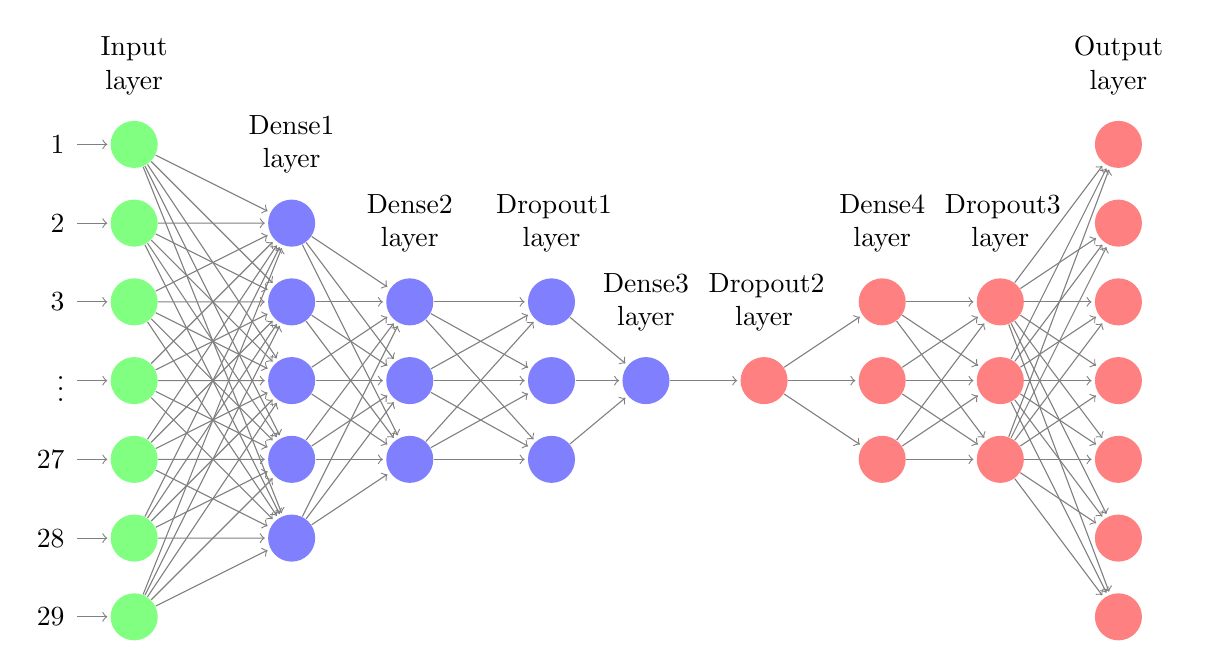
\begin{tikzpicture}[shorten >=1pt,->,draw=black!50, node distance=\layersep]
		\tikzstyle{every pin edge}=[<-,shorten <=1pt]
		\tikzstyle{neuron}=[circle,fill=black!25,minimum size=17pt,inner sep=0pt]
		\tikzstyle{input neuron}=[neuron, fill=green!50];
		\tikzstyle{decoder neuron}=[neuron, fill=red!50];
		\tikzstyle{encoder neuron}=[neuron, fill=blue!50];
		\tikzstyle{annot} = [text width=4em, text centered]
		
		% Draw the input layer nodes
		\foreach \y in {1,...,7}{
			% This is the same as writing \foreach \name / \y in {1/1,2/2,3/3,4/4}
			\ifnum\y<4
			\node[input neuron, pin=left: \y] (I-\y) at (0,-\y) {};
			\fi
			\ifnum\y=4
			\node[input neuron, pin=left: \vdots] (I-\y) at (0,-\y) {};
			\fi
			\ifnum\y=5
			\node[input neuron, pin=left: 27] (I-\y) at (0,-\y) {};
			\fi
			\ifnum\y=6
			\node[input neuron, pin=left: 28] (I-\y) at (0,-\y) {};
			\fi
			\ifnum\y=7
			\node[input neuron, pin=left: 29] (I-\y) at (0,-\y) {};
			\fi
		}
		
		% Draw the Dense_1 layer nodes
		\foreach \y in {2,3,4,5,6}{
			\node[encoder neuron, right of=I-4] (H1-\y) at (\layersep,-\y cm) {};
		}
		% Draw the Dense_2 layer nodes
		\foreach \y in {3,4,5}{
			\node[encoder neuron, right of=H1-3] (H2-\y) at (\layersep*2.5,-\y cm) {};
		}
		% Draw the Dropout_1 layer nodes
		\foreach \y in {3,4,5}{
			\node[encoder neuron, right of=H2-2] (H3-\y) at (\layersep*4.3,-\y cm) {};
		}
		% Draw the Dense_3 layer nodes
		\foreach \y in {4}
		\node[encoder neuron, right of=H3-2] (H4-\y) at (\layersep*5.5,-\y cm) {};
		
		% Draw the Dropout_2 layer nodes
		\foreach \y in {4}
		\node[decoder neuron, right of=H4-1] (H5-\y) at (\layersep*7,-\y cm) {};
		
		% Draw the Dense_4 layer nodes
		\foreach \y in {3,4,5}
		\node[decoder neuron, right of=H5-1] (H6-\y) at (\layersep*8.5,-\y cm) {};
		
		% Draw the Dropout_3 layer nodes
		\foreach \y in {3,4,5}
		\node[decoder neuron, right of=H6-2] (H7-\y) at (\layersep*10,-\y cm) {};
		
		% Draw the output layer node
		\foreach \y in {1,...,7}
		\node[decoder neuron, right of=H7-2] (H8-\y) at (\layersep*11.5,-\y cm){};
		
		% Connect every node in the input layer with every node in the
		% Dense_1 layer.
		\foreach \source in {1,...,7}
		\foreach \dest in {2,3,4,5,6}
		\path (I-\source) edge (H1-\dest);
		% Connect every node in the Dense_1 layer with every node in the
		% Dense_2 layer.
		\foreach \source in {2,3,4,5,6}
		\foreach \dest in {3,4,5}
		\path (H1-\source) edge (H2-\dest);
		% Connect every node in the Dense_2 layer with every node in the
		% Dropout_1 layer.
		\foreach \source in {3,4,5}
		\foreach \dest in {3,4,5}
		\path (H2-\source) edge (H3-\dest);
		% Connect every node in the Dropout_1 layer with every node in the
		% Dense_3 layer.
		\foreach \source in {3,4,5}
		\path (H3-\source) edge (H4-4);
		% Connect every node in the Dense_3 layer with every node in the
		% Dropout_2 layer.
		\path (H4-4) edge (H5-4);
		% Connect every node in the Dropout_2 layer with every node in the
		% Dense_4 layer.
		\foreach \dest in {3,4,5}
		\path (H5-4) edge (H6-\dest);
		% Connect every node in the Dense_4 layer with every node in the
		% Dropout_3 layer.
		\foreach \source in {3,4,5}
		\foreach \dest in {3,4,5}
		\path (H6-\source) edge (H7-\dest);
		% Connect every node in the Dropout_3 layer with every node in the
		% Dense_5 layer.
		\foreach \source in {3,4,5}
		\foreach \dest in {1,...,7}
		\path (H7-\source) edge (H8-\dest);
		
		% Annotate the layers
		\node[annot,above of=H1-2, node distance=1cm] {Dense1 layer};
		\node[annot,above of=H2-3, node distance=1cm] {Dense2 layer};
		\node[annot,above of=H3-3, node distance=1cm] {Dropout1 layer};
		\node[annot,above of=H4-4, node distance=1cm] {Dense3 layer};
		\node[annot,above of=H5-4, node distance=1cm] {Dropout2 layer};
		\node[annot,above of=H6-3, node distance=1cm] {Dense4 layer};
		\node[annot,above of=H7-3, node distance=1cm] {Dropout3 layer};
		\node[annot,above of=I-1] {Input layer};
		\node[annot,above of=H8-1] {Output layer};
	\end{tikzpicture}
\caption{Modelo AE}
\end{figure}

\subsubsection{Denoising AutoEncoder (DAE)}

  DAE es una versi\'{o}n estoc\'{a}stica de AE que reduce el riesgo del aprendizaje de la funci\'{o}n identidad. En AE si existen m\'{a}s capas ocultas que entradas, existe el riesgo de que el algoritmo solo aprenda la funci\'{o}n identidad durante el entrenamiento, es cuando la salida es igual a la entrada, entonces se hace inservible el algoritmo. DAE corrompe aleatoriamente los datos de entrada para reducir este riesgo y aprenda a reconstruir los datos originales a partir de los datos corruptos.
  
  Para la corrupci\'{o}n de los datos se aplicar\'{a} un m\'{e}todo que aplica ruido gaussiano aditivo centrado en cero, esto ayuda a mitigar el \textit{overfitting} y es una opci\'{o}n com\'{u}n para el proceso de corrupci\'{o}n para valores reales de entrada. No se aplicar\'{a} el \textit{dropout} y se utilizar\'{a} el optimizador SGD. En cuanto a las capas se comporta similar al AE: posee la capa de entrada de datos, cuatro capas para el codificador y dos capas para el decodificador. Secuencialmente se conforman de la siguiente forma:

\begin{enumerate}
	\item \textit{Input Layer}: La capa de entrada donde se introducen en la red los datos originales.
	\item \textit{Gaussian Noise}: En esta capa se corrompen los datos y comienza el proceso de codificaci\'{o}n.
	\item \textit{Dense1 Layer}: Se reducen las dimensiones a 14.
	\item \textit{Dense2 Layer}: Se reducen las dimensiones a 7.
	\item \textit{Dense3 Layer}: Se reducen las dimensiones a 1. Termina el proceso de codificaci\'{o}n
	\item \textit{Dense4 Layer}: Se incrementan las dimensiones 7. Comienza la decodificaci\'{o}n.
	\item \textit{Dense5 Layer}: Se incrementan las dimensiones a 29.
	\item \textit{Dense6 Layer} o \textit{Output Layer}: Se comprimen los datos a una dimensi\'{o}n. Termina la decodificaci\'{o}n.
\end{enumerate}

\begin{figure}[h!]
	\centering
	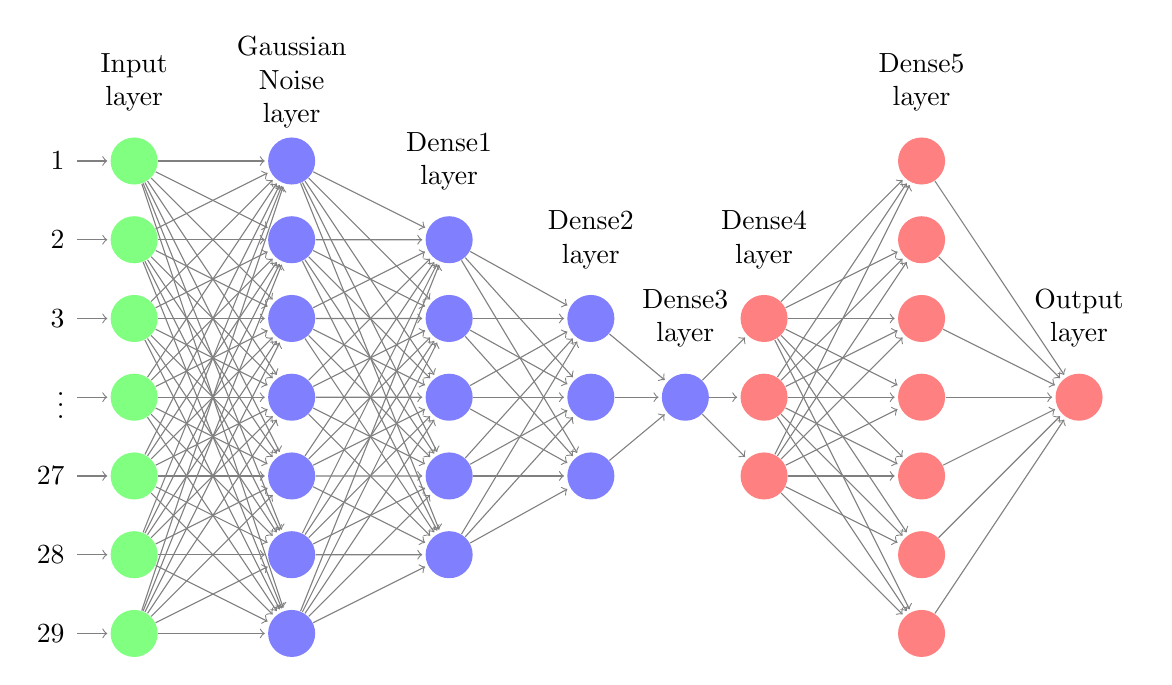
\begin{tikzpicture}[shorten >=1pt,->,draw=black!50, node distance=\layersep]
		\tikzstyle{every pin edge}=[<-,shorten <=1pt]
		\tikzstyle{neuron}=[circle,fill=black!25,minimum size=17pt,inner sep=0pt]
		\tikzstyle{input neuron}=[neuron, fill=green!50];
		\tikzstyle{decoder neuron}=[neuron, fill=red!50];
		\tikzstyle{encoder neuron}=[neuron, fill=blue!50];
		\tikzstyle{annot} = [text width=4em, text centered]
		
		% Draw the input layer nodes
		\foreach \y in {1,...,7}{
			% This is the same as writing \foreach \name / \y in {1/1,2/2,3/3,4/4}
			\ifnum\y<4
			\node[input neuron, pin=left: \y] (I-\y) at (0,-\y) {};
			\fi
			\ifnum\y=4
			\node[input neuron, pin=left: \vdots] (I-\y) at (0,-\y) {};
			\fi
			\ifnum\y=5
			\node[input neuron, pin=left: 27] (I-\y) at (0,-\y) {};
			\fi
			\ifnum\y=6
			\node[input neuron, pin=left: 28] (I-\y) at (0,-\y) {};
			\fi
			\ifnum\y=7
			\node[input neuron, pin=left: 29] (I-\y) at (0,-\y) {};
			\fi
		}
		
		% Draw the Gaussian_Noise nodes
		\foreach \y in {1,...,7}
		\node[encoder neuron] (H1-\y) at (\layersep*2,-\y) {};
		
		% Draw the Dense_1 layer nodes
		\foreach \y in {2,3,4,5,6}{
			\node[encoder neuron, right of=1-4] (H2-\y) at (\layersep*3,-\y cm) {};
		}
		% Draw the Dense_2 layer nodes
		\foreach \y in {3,4,5}{
			\node[encoder neuron, right of=H2-4] (H3-\y) at (\layersep*4.8,-\y cm) {};
		}
		% Draw the Dense_3 layer nodes
		\foreach \y in {4}
		\node[encoder neuron, right of=H3-4] (H4-\y) at (\layersep*6,-\y cm) {};
		
		% Draw the Dense_4 layer nodes
		\foreach \y in {3,4,5}
		\node[decoder neuron, right of=H4-4] (H5-\y) at (\layersep*7,-\y cm) {};
		
		% Draw the Dense_5 layer node
		\foreach \y in {1,...,7}
		\node[decoder neuron, right of=H5-4] (H6-\y) at (\layersep*9,-\y cm){};
		
		% Draw the Dense_6 layer node
		\node[decoder neuron, right of=H6-4] (O-4) at (\layersep*11,-4 cm){};
		
		% Connect every node in the input layer with every node in the
		% Gaussian_Noise layer.
		\foreach \source in {1,...,7}
		\foreach \dest in {1,...,7}
		\path (I-\source) edge (H1-\dest);
		% Connect every node in the Gaussian_Noise layer with every node in the
		% Dense_1 layer.
		\foreach \source in {1,...,7}
		\foreach \dest in {2,3,4,5,6}
		\path (H1-\source) edge (H2-\dest);
		% Connect every node in the Dense_1 layer with every node in the
		% Dense_2 layer.
		\foreach \source in {2,3,4,5,6}
		\foreach \dest in {3,4,5}
		\path (H2-\source) edge (H3-\dest);
		% Connect every node in the Dense_2 layer with every node in the
		% Dense_3 layer.
		\foreach \source in {3,4,5}
		\path (H3-\source) edge (H4-4);
		% Connect every node in the Denes_3 layer with every node in the
		% Dense_4 layer.
		\foreach \dest in {3,4,5}
		\path (H4-4) edge (H5-\dest);
		% Connect every node in the Dense_4 layer with every node in the
		% Dense_5 layer.
		\foreach \source in {3,4,5}
		\foreach \dest in {1,...,7}
		\path (H5-\source) edge (H6-\dest);
		
		% Connect every node in the Dense_5 layer with every node in the
		% Dense_6 layer.
		\foreach \source in {1,...,7}
		\path (H6-\source) edge (O-4);
		
		% Annotate the layers
		\node[annot,above of=H1-1, node distance=1cm] {Gaussian Noise layer};
		\node[annot,above of=H2-2, node distance=1cm] {Dense1 layer};
		\node[annot,above of=H3-3, node distance=1cm] {Dense2 layer};
		\node[annot,above of=H4-4, node distance=1cm] {Dense3 layer};
		\node[annot,above of=H5-3, node distance=1cm] {Dense4 layer};
		\node[annot,above of=H6-1, node distance=1cm] {Dense5 layer};
		\node[annot,above of=I-1] {Input layer};
		\node[annot,above of=O-4] {Output layer};
	\end{tikzpicture}
\caption{Modelo DAE}
\end{figure}

\subsubsection{Convolutional Neural Network (CNN)}

  La CNN es una red multicapa que consta de capas convolucionales y de reducci\'{o}n alternada, y al final tiene capas de conexi\'{o}n total como una red perceptr\'{o}n multicapa. Son capaces de detectar caracter\'{i}sticas simples y componer en caracter\'{i}sticas m\'{a}s complejas hasta detectar lo que se busca. Su principal ventaja es que cada parte de la red se le entrena para realizar una tarea, esto reduce significativamente el n\'{u}mero de capas ocultas, por lo que el entrenamiento es m\'{a}s r\'{a}pido.
  
  Al aplicar CNN para la clasificaci\'{o}n se realiza en dos fases: la primera fase es la de extracci\'{o}n de caracter\'{i}sticas, la cual est\'{a} compuesta por neuronas convolucionales y de reducci\'{o}n de muestreo; y la segunda fase es la clasificaci\'{o}n final a partir de las caracter\'{i}sticas extra\'{i}das.
  
  La primera fase se compone de capas alternas de neuronas convolucionales y neuronas de reducci\'{o}n de muestreo. A medida que los datos avanzan por esta fase, van perdiendo dimensionalidad, siendo las neuronas de las capas finales poco sensibles a perturbaciones en los datos de entrada, al mismo tiempo se activan por caracter\'{i}sticas m\'{a}s complejas. Las neuronas son remplazadas por procesadores en matriz que realizan una operaci\'{o}n sobre los datos que pasan por ellas en vez de un \'{u}nico valor num\'{e}rico. Matem\'{a}ticamente la salida $S_{j}$ de una neurona $j$, es una matriz que se calcula por medio de la combinaci\'{o}n lineal de las salidas $S_{i}$ de las neuronas de la capa anterior, cada una de ellas operadas con el n\'{u}cleo de convolucional $K_{ij}$ correspondiente a esa conexi\'{o}n. Esta cantidad es sumada a una parcialidad $b_{j}$ y luego se pasa por una funci\'{o}n de activaci\'{o}n $g$. Pr\'{a}cticamente la ecuaci\'{o}n queda de la siguiente manera:

\begin{equation}
	S_{j}=g(b_{j}+\sum_{i}(K_{ij}\otimes Y_{i})
\end{equation}

  Las CNN anteriormente utilizaban el proceso de submuestreo para realizar la reducci\'{o}n de muestreo, pero con estudios recientes se han encontrado otras operaciones como \textit{max-pooling}, que encuentra el valor m\'{a}ximo entre una ventana de muestra y pasa este valor como resumen de caracter\'{i}sticas sobre esta \'{a}rea. Esto permite que el tama\~{n}o de los datos se reduce por un factor igual al tama\~{n}o de la ventana de muestra sobre la cual se opera.
  
  Al concluir con las extracciones de caracter\'{i}sticas, se procede a la fase de clasificaci\'{o}n, gracias a que los datos han sido depurados hasta una serie de caracter\'{i}sticas \'{u}nicas para los datos de entrada. Las neuronas en esta fase funcionan de manera similar a las de un perceptr\'{o}n multicapa. La salida $y_{j}$ de una neurona $j$ se calcula a partir de las salidas $y_{i}$ de las neuronas de la capa anterior cada una de ellas multiplicadas con el peso $w_{ij}$ correspondiente. Esta cantidad es sumada a una parcialidad $b_{j}$ y luego se pasa por una funci\'{o}n de activaci\'{o}n $g$. La ecuaci\'{o}n queda de esta forma:

\begin{equation}
	y_{i}=g(b_{j}+\sum_{i}w_{ij}y_{i})
\end{equation}

  Para el proyecto se desarrollar\'{a} una CNN con dos fases de extracci\'{o}n de caracter\'{i}sticas, en cada una se aplicar\'{a} la convoluci\'{o}n, un \textit{BatchNormalization} y un \textit{Dropout}. Luego una fase de clasificaci\'{o}n donde se aplicar\'{a} un \textit{Flatten} para reducir los datos a una dimensi\'{o}n, una capa \textit{Dense} para incrementar las dimensiones a 64 y por \'{u}ltimo un \textit{Dropout}. Y, por \'{u}ltimo, una capa de salida; adem\'{a}s se aplicar\'{a} Adam como optimizador. Las capas en orden se describen a continuaci\'{o}n:
  
  \begin{enumerate}
  	\item \textit{Input Layer}: Se introducen los datos con dimensi\'{o}n $(None, 29, 1)$.
  	\item \textit{Conv1D-1 Layer}: Comienza la primera fase de extracci\'{o}n de caracter\'{i}sticas, introduciendo una capa convolucional que transforma las dimensiones a $(None, 28, 32)$.
  	\item \textit{Batch-Normalization-1 Layer}: Se aplica el regularizador para normalizar los datos.
  	\item \textit{Dropout-1 Layer}: Se aplica el regularizador para eliminar modelos para evitar el \textit{overfitting}, y culmina la primera fase de extracci\'{o}n de caracter\'{i}sticas.
  	\item \textit{Conv1D-2 Layer}: Se aplica una capa de convoluci\'{o}n y comienza la segunda fase de extracci\'{o}n de caracter\'{i}sticas. La dimensi\'{o}n de los datos se transforma a $(None, 27, 64)$.
  	\item \textit{Batch-Normalization-2 Layer}: Se aplica el regularizador para normalizar los datos.
  	\item \textit{Dropout-2 Layer}: Se aplica el regularizador para eliminar modelos para evitar el \textit{overfitting} y termina la segunda fase de extracci\'{o}n.
  	\item \textit{Flatten Layer}: Se descomponen los datos a tener la dimensi\'{o}n $(None, 1728)$ y comienza la fase de clasificaci\'{o}n.
  	\item \textit{Dense-1 Layer}: Se comprimen los datos hasta obtener las dimensiones $(None, 64)$.
  	\item \textit{Dropout-3 Layer}: Se eliminan modelos para evitar el \textit{overfitting}.
  	\item \textit{Dense-2 Layer} o \textit{Output Layer}: Se comprimen los datos una dimensi\'{o}n obteniendo los datos clasificados y terminando la fase de clasificaci\'{o}n.
  \end{enumerate}

\begin{figure}[h!]
	\centering
	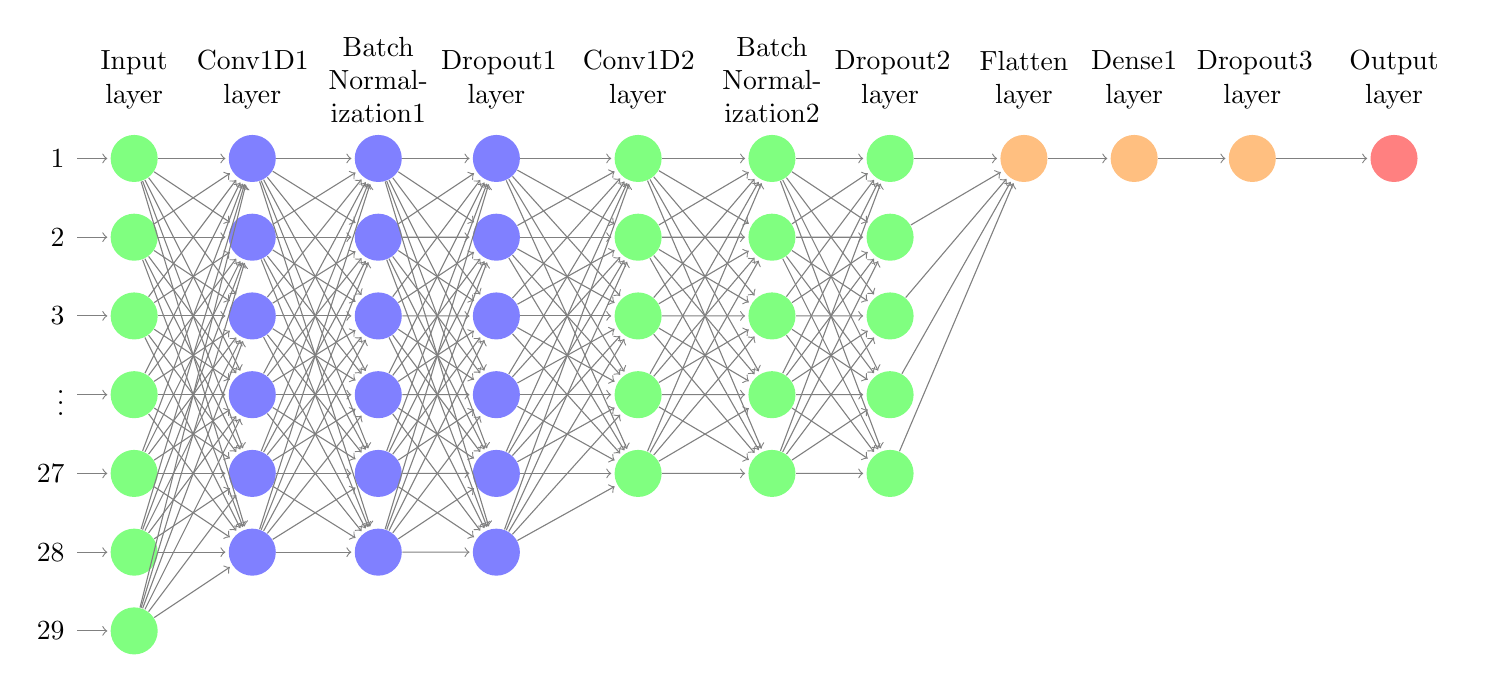
\begin{tikzpicture}[shorten >=1pt,->,draw=black!50, node distance=\layersep]
		\tikzstyle{every pin edge}=[<-,shorten <=1pt]
		\tikzstyle{neuron}=[circle,fill=black!25,minimum size=17pt,inner sep=0pt]
		\tikzstyle{input neuron}=[neuron, fill=green!50];
		\tikzstyle{fase1 neuron}=[neuron, fill=blue!50];
		\tikzstyle{fase2 neuron}=[neuron, fill=green!50];
		\tikzstyle{fase3 neuron}=[neuron, fill=orange!50];
		\tikzstyle{output neuron}=[neuron, fill=red!50];
		\tikzstyle{annot} = [text width=4em, text centered]
		
		% Draw the input layer nodes
		\foreach \y in {1,...,7}{
			% This is the same as writing \foreach \name / \y in {1/1,2/2,3/3,4/4}
			\ifnum\y<4
			\node[input neuron, pin=left: \y] (I-\y) at (0,-\y) {};
			\fi
			\ifnum\y=4
			\node[input neuron, pin=left: \vdots] (I-\y) at (0,-\y) {};
			\fi
			\ifnum\y=5
			\node[input neuron, pin=left: 27] (I-\y) at (0,-\y) {};
			\fi
			\ifnum\y=6
			\node[input neuron, pin=left: 28] (I-\y) at (0,-\y) {};
			\fi
			\ifnum\y=7
			\node[input neuron, pin=left: 29] (I-\y) at (0,-\y) {};
			\fi
		}
		
		% Draw the Conv1D_1 nodes
		\foreach \y in {1,...,6}
		\node[fase1 neuron, right of=I-4] (H1-\y) at (\layersep*0.5,-\y) {};
		
		% Draw the Batch_Normalization_1 nodes
		\foreach \y in {1,...,6}
		\node[fase1 neuron, right of=H1-4] (H2-\y) at (\layersep*2.1,-\y) {};
		
		% Draw the Dropout_1 layer nodes
		\foreach \y in {1,...,6}
		\node[fase1 neuron, right of=H2-4] (H3-\y) at (\layersep*3.6,-\y cm) {};
		
		% Draw the Conv1D_2 nodes
		\foreach \y in {1,...,5}
		\node[fase2 neuron, right of=H3-4] (H4-\y) at (\layersep*5.4,-\y cm) {};
		
		% Draw the Batch_Normalization_2 nodes
		\foreach \y in {1,...,5}
		\node[fase2 neuron, right of=H4-4] (H5-\y) at (\layersep*7.1,-\y) {};
		
		% Draw the Dropout_2 layer nodes
		\foreach \y in {1,...,5}
		\node[fase2 neuron, right of=H5-4] (H6-\y) at (\layersep*8.6,-\y cm) {};
		
		% Draw the Flatten layer nodes
		\node[fase3 neuron, right of=H6-4] (H7-1) at (\layersep*10.3,-1 cm) {};
		
		% Draw the Dense_1 layer nodes
		\node[fase3 neuron, right of=H7-1] (H8-1) at (\layersep*11.7,-1 cm) {};
		
		% Draw the Dropout_3 layer nodes
		\node[fase3 neuron, right of=H8-1] (H9-1) at (\layersep*13.2,-1 cm) {};
		
		% Draw the Dense_2 layer nodes
		\node[output neuron, right of=H9-1] (H10-1) at (\layersep*15,-1 cm) {};
		
		% Connect every node in the input layer with every node in the
		% Conv1D_2 layer.
		\foreach \source in {1,...,7}
		\foreach \dest in {1,...,6}
		\path (I-\source) edge (H1-\dest);
		% Connect every node in the Conv1D_2 layer with every node in the
		% Batch_Normalization_1 layer.
		\foreach \source in {1,...,6}
		\foreach \dest in {1,...,6}
		\path (H1-\source) edge (H2-\dest);
		% Connect every node in the Batch_Normalization_1 layer with every node in the
		% Dropout_1 layer.
		\foreach \source in {1,...,6}
		\foreach \dest in {1,...,6}
		\path (H2-\source) edge (H3-\dest);
		% Connect every node in the Dropout_1 layer with every node in the
		% Conv1D_2 layer.
		\foreach \source in {1,...,6}
		\foreach \dest in {1,...,5}
		\path (H3-\source) edge (H4-\dest);
		% Connect every node in the Conv1D_2 layer with every node in the
		% Batch_Normalization_1 layer.
		\foreach \source in {1,...,5}
		\foreach \dest in {1,...,5}
		\path (H4-\source) edge (H5-\dest);
		% Connect every node in the Batch_Normalization_1 layer with every node in the
		% Dropout_2 layer.
		\foreach \source in {1,...,5}
		\foreach \dest in {1,...,5}
		\path (H5-\source) edge (H6-\dest);
		% Connect every node in the Dropout_2 layer with every node in the
		% Flatten layer.
		\foreach \source in {1,...,5}
		\path (H6-\source) edge (H7-1);
		% Connect every node in the Flatten layer with every node in the
		% Dense_1 layer.
		\path (H7-1) edge (H8-1);
		% Connect every node in the Dense_1 layer with every node in the
		% Dropout_3 layer.
		\path (H8-1) edge (H9-1);
		% Connect every node in the Dropout_3 layer with every node in the
		% Dense_2 layer.
		\path (H9-1) edge (H10-1);
		
		% Annotate the layers
		\node[annot,above of=H1-1, node distance=1cm] {Conv1D1 layer};
		\node[annot,above of=H2-1, node distance=1cm] {Batch Normalization1};
		\node[annot,above of=H3-1, node distance=1cm] {Dropout1 layer};
		\node[annot,above of=H4-1, node distance=1cm] {Conv1D2 layer};
		\node[annot,above of=H5-1, node distance=1cm] {Batch Normalization2};
		\node[annot,above of=H6-1, node distance=1cm] {Dropout2 layer};
		\node[annot,above of=H7-1, node distance=1cm] {Flatten layer};
		\node[annot,above of=H8-1, node distance=1cm] {Dense1 layer};
		\node[annot,above of=H9-1, node distance=1cm] {Dropout3 layer};
		\node[annot,above of=I-1] {Input layer};
		\node[annot,above of=H10-1] {Output layer};
	\end{tikzpicture}
	\caption{Modelo CNN}
\end{figure}

\subsubsection{Backpropagation Neural Network (BPNN)}

  En las redes neuronales se introducen los datos por la capa de entrada y se propagan hacia adelante atravesando las capas ocultas hasta llegar a la capa de salida, obteniendo el resultado final. Este resultado se compara con los valores reales para calcular el error que se comete, y propagar este error hacia atr\'{a}s a trav\'{e}s de la red neuronal, permitiendo ajustar los pesos durante el proceso de entrenamiento. Uno de los m\'{e}todos para realizar esta operaci\'{o}n es \textit{backpropagation}.
  
  \textit{Backpropagation} se activa luego de que la informaci\'{o}n llega a la capa de salida y se mide el error que se ha cometido en esa observaci\'{o}n. En la propagaci\'{o}n hacia atr\'{a}s, se van actualizando los pesos de cada conexi\'{o}n neuronal, dependiendo de la responsabilidad del peso actualizado en el error cometido. Este proceso se repite para el conjunto de observaciones, al pasar todas las observaciones por la red neuronal, se completa una \'{e}poca.
  
  Matem\'{a}ticamente el nodo de una red neuronal se podr\'{i}a representar como $a_{i}^{k}$ donde $i$ es el lugar que representa el nodo dentro de una capa y $k$ representa la capa en que se encuentra el nodo. El peso de las conexiones se representa como $w_{ji}^{k}$ donde $i$ indica el n\'{u}mero de la neurona dentro de la capa final de la conexi\'{o}n, e $j$ indica el n\'{u}mero de la neurona de la capa inicial de la conexi\'{o}n. Entonces la ecuaci\'{o}n para calcular \textit{backpropagation} queda de la siguiente forma:

\begin{align}
	a_{i}^{k}=f(u_{i}^{k}+\sum_{j=1}^{n_{k}-1}a_{j}^{k-1}w_{ji}^{k-1}) \\
	i = 1, ...., n_{k}
\end{align}

  El algoritmo BPNN que se utilizar\'{a} en el proyecto hace uso del optimizador Adam y posee solamente $5$ capas, incluyendo la de entrada y salida. A continuaci\'{o}n, la secuencia de las capas:
  
  \begin{enumerate}
  	\item \textit{Input layer}: se introducen el conjunto de datos originales sin clasificar.
  	\item \textit{Dense-1 layer}: se comprimen los datos a 14 dimensiones.
  	\item \textit{Dense-2 layer}: se comprimen los datos a 2 dimensiones.
  	\item \textit{Dense-3 layer}: se descomprimen los datos a 14 dimensiones.
  	\item \textit{Dense-4 layer} o \textit{Output layer}: se comprimen los datos a una dimensi\'{o}n y termina la clasificaci\'{o}n de los datos.
  \end{enumerate}

\begin{figure}[h!]
	\centering
	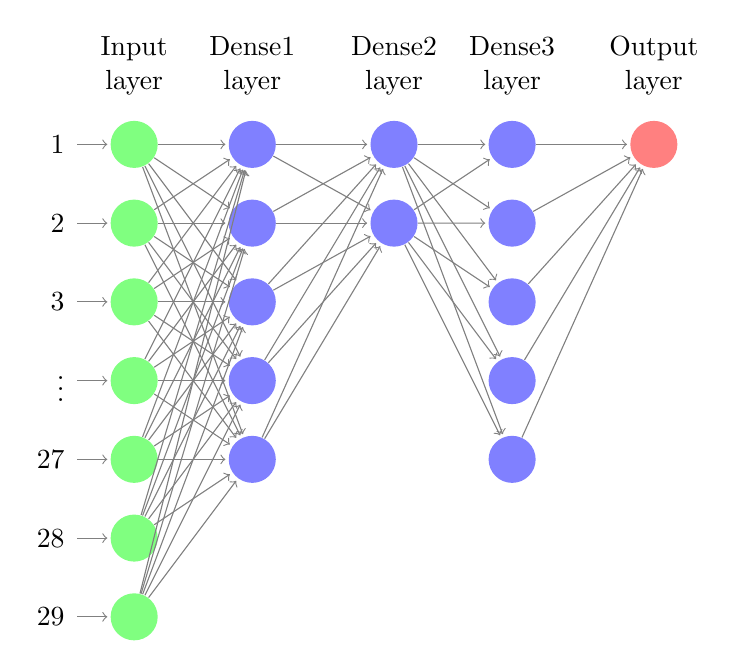
\begin{tikzpicture}[shorten >=1pt,->,draw=black!50, node distance=\layersep]
		\tikzstyle{every pin edge}=[<-,shorten <=1pt]
		\tikzstyle{neuron}=[circle,fill=black!25,minimum size=17pt,inner sep=0pt]
		\tikzstyle{input neuron}=[neuron, fill=green!50];
		\tikzstyle{hidden neuron}=[neuron, fill=blue!50];
		\tikzstyle{output neuron}=[neuron, fill=red!50];
		\tikzstyle{annot} = [text width=4em, text centered]
		
		% Draw the input layer nodes
		\foreach \y in {1,...,7}{
			% This is the same as writing \foreach \name / \y in {1/1,2/2,3/3,4/4}
			\ifnum\y<4
			\node[input neuron, pin=left: \y] (I-\y) at (0,-\y) {};
			\fi
			\ifnum\y=4
			\node[input neuron, pin=left: \vdots] (I-\y) at (0,-\y) {};
			\fi
			\ifnum\y=5
			\node[input neuron, pin=left: 27] (I-\y) at (0,-\y) {};
			\fi
			\ifnum\y=6
			\node[input neuron, pin=left: 28] (I-\y) at (0,-\y) {};
			\fi
			\ifnum\y=7
			\node[input neuron, pin=left: 29] (I-\y) at (0,-\y) {};
			\fi
		}
		
		% Draw the Dense_1 nodes
		\foreach \y in {1,...,5}
		\node[hidden neuron, right of=I-4] (H1-\y) at (\layersep*0.5,-\y) {};
		
		% Draw the Dense_2 nodes
		\foreach \y in {1,2}
		\node[hidden neuron, right of=H1-3] (H2-\y) at (\layersep*2.3,-\y) {};
		
		% Draw the Dense_3 layer nodes
		\foreach \y in {1,...,5}
		\node[hidden neuron, right of=H2-2] (H3-\y) at (\layersep*3.8,-\y cm) {};
		
		% Draw the Dense_4 nodes
		\node[output neuron, right of=H3-3] (O-1) at (\layersep*5.6,-1 cm) {};
		
		% Connect every node in the input layer with every node in the
		% Dense_1 layer.
		\foreach \source in {1,...,7}
		\foreach \dest in {1,...,5}
		\path (I-\source) edge (H1-\dest);
		% Connect every node in the Dense_1 layer with every node in the
		% Dense_2 layer.
		\foreach \source in {1,...,5}
		\foreach \dest in {1,2}
		\path (H1-\source) edge (H2-\dest);
		% Connect every node in the Dense_2 layer with every node in the
		% Dense_3 layer.
		\foreach \source in {1,2}
		\foreach \dest in {1,...,5}
		\path (H2-\source) edge (H3-\dest);
		% Connect every node in the Dense_3 layer with every node in the
		% Dense_4 layer.
		\foreach \source in {1,...,5}
		\path (H3-\source) edge (O-1);
		
		% Annotate the layers
		\node[annot,above of=H1-1, node distance=1cm] {Dense1 layer};
		\node[annot,above of=H2-1, node distance=1cm] {Dense2 layer};
		\node[annot,above of=H3-1, node distance=1cm] {Dense3 layer};
		\node[annot,above of=I-1] {Input layer};
		\node[annot,above of=O-1] {Output layer};
	\end{tikzpicture}
\caption{Modelo BPNN}
\end{figure}

\subsubsection{Recurrent Neural Network (RNN)}

    RNN es un modelo supervisado de aprendizaje profundo conde la actual salida depende del valor actual y de las entradas anteriores usando \textit{backpropagation} a trav\'{e}s del tiempo $t$ en que se realizan las transacciones. Matem\'{a}ticamente, se define $X_{t}$ como los datos de entrada en el instante de tiempo $t$, $H_{t}$ como el paso de tiempo de la capa oculta, y $y_{t}$ como la salida de los datos en el instante de tiempo. En el procesamiento de los datos desde la entrada a la salida intervienen los vectores de peso dependiendo de las capas, para mejor apreciaci\'{o}n se muestran en el gr\'{a}fico siguiente:
    
    \begin{figure}[h!]
    	\centering
    	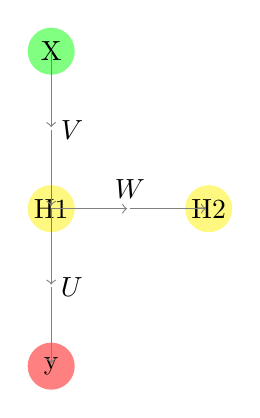
\begin{tikzpicture}[shorten >=1pt,->,draw=black!50, node distance=\layersep]
    		\tikzstyle{every pin edge}=[<-,shorten <=1pt]
    		\tikzstyle{neuron}=[circle,fill=black!25,minimum size=17pt,inner sep=0pt]
    		\tikzstyle{input neuron}=[neuron, fill=green!50];
    		\tikzstyle{hidden neuron}=[neuron, fill=yellow!50];
    		\tikzstyle{output neuron}=[neuron, fill=red!50];
    		\tikzstyle{annot} = [text width=4em, text centered]
    		
    		\node[input neuron] (I-1) at (0,0) {X};
    		\node[hidden neuron] (H-1) at (0,-2) {H1};
    		\draw (0,0) -- (0,-1) node(I-H11)[right] {$V$};
    		\draw (0,-1) -- (0,-2) node(I-H12)[right] {$$};
    		\node[output neuron] (O-1) at (0,-4) {y};
    		\draw (0,-2) -- (0,-3) node(H1-O1)[right] {$U$};
    		\draw (0,-3) -- (0,-4) node(H1-O2)[right] {$$};
    		\node[hidden neuron] (H-2) at (2,-2) {H2};
    		\draw (0,-2) -- (1,-2) node(H1-H21)[above] {$W$};
    		\draw (1,-2) -- (2,-2) node(H1-H22)[right] {$$};
    		
    	\end{tikzpicture}
    	\caption{Funcionamiento RNN}
    \end{figure}

    $V$ es el vector peso para la capa oculta, $U$ es el vector peso para la capa de salida y $W$ es el mismo vector peso para los diferentes instantes de tiempo. Teniendo en cuenta esto, se puede calcular la capa oculta y la salida teniendo en cuenta estas variables y la funci\'{o}n de activaci\'{o}n $\sigma$, para ello se usan las siguientes ecuaciones:
    
    \begin{align}
    	H_{t}=\sigma(UX_{t}+WH_{t-1})\\
    	y_{t}=Softmax(VH_{t})
    \end{align}

    RNN aplica el algoritmo \textit{backward propagation} para actualizar los pesos, sus fundamentos se exponen en el siguiente algoritmo LSTM.
  
    El algoritmo RNN a aplicar en el proyecto est\'{a} compuesto con una capa de RNN para el tratamiento de la informaci\'{o}n teniendo en cuenta los instantes de tiempo. Se Aplicar\'{a}n tres capas regularizadoras \textit{Dropout} no consecutivas con el objetivo de evitar el \textit{overfitting} y capas \textit{Dense} para redimensionar los datos, adem\'{a}s, se aplicar\'{a} el optimizador Adam. En conclusi\'{o}n, el algoritmo est\'{a} compuesto por $8$ capas divididos en: $1$ capa de salida, $1$ capa de RNN, $5$ capas de clasificaci\'{o}n y $1$ capa de salida. La arquitectura es la siguiente de forma secuencial:

\begin{enumerate}
	\item \textit{Input Layer}: Se introducen los datos originales con los pasos de tiempos.
	\item \textit{RNN layer}: Se aplica el proceso correspondiente al \textit{backpropagation} con pasos de tiempo.
	\item \textit{Dropout-1 layer}: Se aplica el regularizador \textit{Dropout} y comienza la clasificaci\'{o}n.
	\item \textit{Dense-1 layer}: Se comprimen los datos a 14 dimensiones.
	\item \textit{Dropout-2 layer}: Se aplica el nuevamente el regularizador.
	\item \textit{Dense-2 layer}: Se vuelve a aplicar la compresi\'{o}n de los datos.
	\item \textit{Dropout-3 layer}: Se vuelve a aplicar el regularizador.
	\item \textit{Dense-3 layer} o \textit{Output layer}: Se comprimen los datos a una dimensi\'{o}n terminando con la clasificaci\'{o}n de los datos.
\end{enumerate}

\begin{figure}[h!]
	\centering
	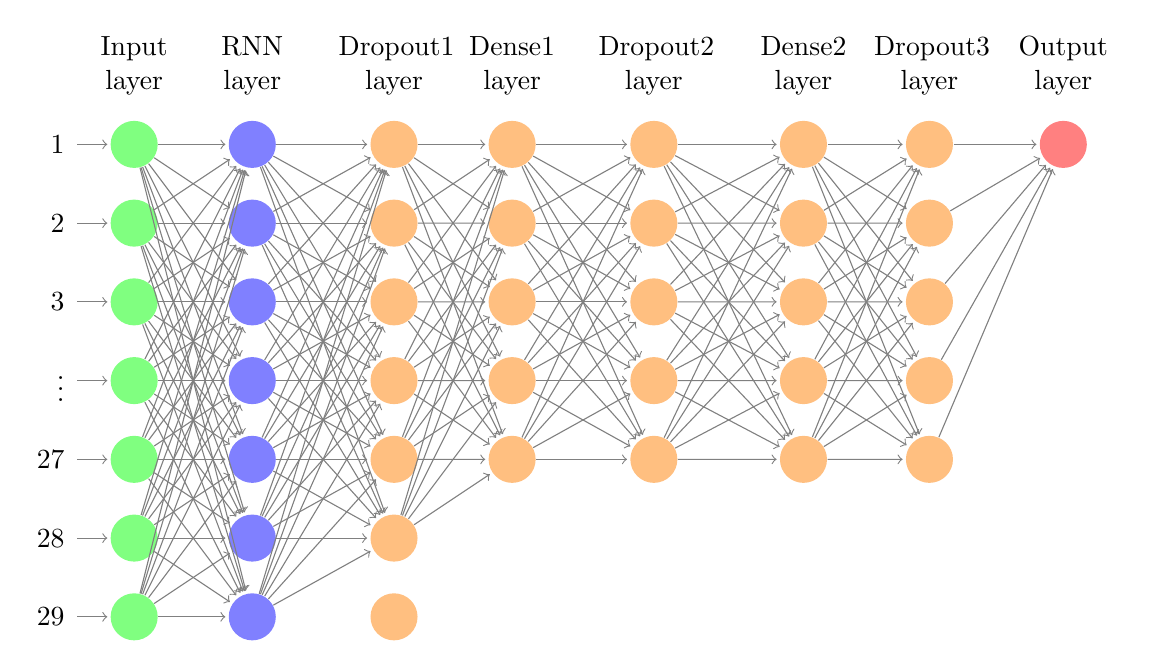
\begin{tikzpicture}[shorten >=1pt,->,draw=black!50, node distance=\layersep]
		\tikzstyle{every pin edge}=[<-,shorten <=1pt]
		\tikzstyle{neuron}=[circle,fill=black!25,minimum size=17pt,inner sep=0pt]
		\tikzstyle{input neuron}=[neuron, fill=green!50];
		\tikzstyle{fase1 neuron}=[neuron, fill=blue!50];
		\tikzstyle{fase2 neuron}=[neuron, fill=orange!50];
		\tikzstyle{output neuron}=[neuron, fill=red!50];
		\tikzstyle{annot} = [text width=4em, text centered]
		
		% Draw the input layer nodes
		\foreach \y in {1,...,7}{
			% This is the same as writing \foreach \name / \y in {1/1,2/2,3/3,4/4}
			\ifnum\y<4
			\node[input neuron, pin=left: \y] (I-\y) at (0,-\y) {};
			\fi
			\ifnum\y=4
			\node[input neuron, pin=left: \vdots] (I-\y) at (0,-\y) {};
			\fi
			\ifnum\y=5
			\node[input neuron, pin=left: 27] (I-\y) at (0,-\y) {};
			\fi
			\ifnum\y=6
			\node[input neuron, pin=left: 28] (I-\y) at (0,-\y) {};
			\fi
			\ifnum\y=7
			\node[input neuron, pin=left: 29] (I-\y) at (0,-\y) {};
			\fi
		}
		
		% Draw the RNN nodes
		\foreach \y in {1,...,7}
		\node[fase1 neuron, right of=I-4] (H1-\y) at (\layersep*0.5,-\y) {};
		
		% Draw the Dropout_1 nodes
		\foreach \y in {1,...,7}
		\node[fase2 neuron, right of=H1-4] (H2-\y) at (\layersep*2.3,-\y) {};
		
		% Draw the Dense_1 layer nodes
		\foreach \y in {1,...,5}
		\node[fase2 neuron, right of=H2-4] (H3-\y) at (\layersep*3.8,-\y cm) {};
		
		% Draw the Dropout_2 nodes
		\foreach \y in {1,...,5}
		\node[fase2 neuron, right of=H3-3] (H4-\y) at (\layersep*5.6,-\y cm) {};
		
		% Draw the Dense_2 nodes
		\foreach \y in {1,...,5}
		\node[fase2 neuron, right of=H4-3] (H5-\y) at (\layersep*7.5,-\y) {};
		
		% Draw the Dropout_3 layer nodes
		\foreach \y in {1,...,5}
		\node[fase2 neuron, right of=H5-3] (H6-\y) at (\layersep*9.1,-\y cm) {};
		
		% Draw the Dense_3 layer nodes
		\node[output neuron, right of=H6-3] (H7-1) at (\layersep*10.8,-1 cm) {};
		
		% Connect every node in the input layer with every node in the
		% RNN layer.
		\foreach \source in {1,...,7}
		\foreach \dest in {1,...,7}
		\path (I-\source) edge (H1-\dest);
		% Connect every node in the RNN layer with every node in the
		% Dropout_1 layer.
		\foreach \source in {1,...,7}
		\foreach \dest in {1,...,6}
		\path (H1-\source) edge (H2-\dest);
		% Connect every node in the Dropout_1 layer with every node in the
		% Dense_1 layer.
		\foreach \source in {1,...,6}
		\foreach \dest in {1,...,5}
		\path (H2-\source) edge (H3-\dest);
		% Connect every node in the Dense_1 layer with every node in the
		% Dropout_2 layer.
		\foreach \source in {1,...,5}
		\foreach \dest in {1,...,5}
		\path (H3-\source) edge (H4-\dest);
		% Connect every node in the Dropout_2 layer with every node in the
		% Dense_2 layer.
		\foreach \source in {1,...,5}
		\foreach \dest in {1,...,5}
		\path (H4-\source) edge (H5-\dest);
		% Connect every node in the Dense_2 layer with every node in the
		% Dropout_3 layer.
		\foreach \source in {1,...,5}
		\foreach \dest in {1,...,5}
		\path (H5-\source) edge (H6-\dest);
		% Connect every node in the Dropout_3 layer with every node in the
		% Dense_3 layer.
		\foreach \source in {1,...,5}
		\path (H6-\source) edge (H7-1);
		
		
		% Annotate the layers
		\node[annot,above of=H1-1, node distance=1cm] {RNN layer};
		\node[annot,above of=H2-1, node distance=1cm] {Dropout1 layer};
		\node[annot,above of=H3-1, node distance=1cm] {Dense1 layer};
		\node[annot,above of=H4-1, node distance=1cm] {Dropout2 layer};
		\node[annot,above of=H5-1, node distance=1cm] {Dense2 layer};
		\node[annot,above of=H6-1, node distance=1cm] {Dropout3 layer};
		\node[annot,above of=I-1] {Input layer};
		\node[annot,above of=H7-1] {Output layer};
	\end{tikzpicture}
\caption{Modelo RNN}
\end{figure}

\subsubsection{Long Short Term Memory (LSTM)}

    LSTM soluciona el problema de los gradientes que desaparecen y explotan de RNN al poseer una mayor memoria para almacenar los vectores de peso. La siguiente figura muestra la arquitectura del funcionamiento del algoritmo:
    
    \begin{figure}[h!]
    	\centering
    	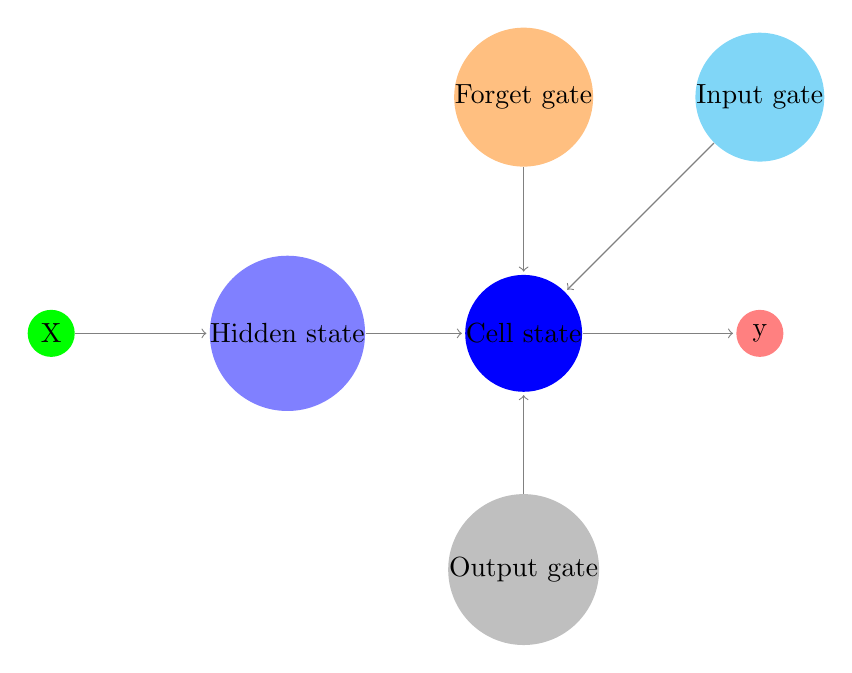
\begin{tikzpicture}[shorten >=1pt,->,draw=black!50, node distance=\layersep]
    		\tikzstyle{every pin edge}=[<-,shorten <=1pt]
    		\tikzstyle{neuron}=[circle,fill=black!25,minimum size=17pt,inner sep=0pt]
    		\tikzstyle{input neuron}=[neuron, fill=green!100];
    		\tikzstyle{hidden state}=[neuron, fill=blue!50];
    		\tikzstyle{forget gate}=[neuron, fill=orange!50];
    		\tikzstyle{input gate}=[neuron, fill=cyan!50];
    		\tikzstyle{output gate}=[neuron, fill=gray!50];
    		\tikzstyle{cell state}=[neuron, fill=blue!100];
    		\tikzstyle{output neuron}=[neuron, fill=red!50];
    		\tikzstyle{annot} = [text width=4em, text centered]
    		
    		\node[input neuron] (I-1) at (0,-4) {X};
    		\node[hidden state] (H-1) at (\layersep*3,-4) {Hidden state};
    		\node[forget gate] (G-1) at (\layersep*6,-1) {Forget gate};
    		\node[input gate] (G-2) at (\layersep*9,-1) {Input gate};
    		\node[output gate] (G-3) at (\layersep*6,-7) {Output gate};
    		\node[cell state] (H-2) at (\layersep*6,-4) {Cell state};
    		\node[output neuron] (O-1) at (\layersep*9,-4) {y};
    		
    		\path (I-1) edge (H-1);
    		\path (H-1) edge (H-2);
    		\path (G-1) edge (H-2);
    		\path (G-2) edge (H-2);
    		\path (G-3) edge (H-2);
    		\path (H-2) edge (O-1);
    	\end{tikzpicture}
    \caption{Funcionamiento de LSTM}
    \end{figure}

  En la figura se denota $X$ como el conjunto de datos originales sin clasificar, este conjunto pasa al estado oculto (\textit{Hidden state}) que es similar a la capa RNN donde se alimenta de las entradas anteriores. Los datos pasan a tres puertas: \textit{Input gate}, \textit{Forget gate} y \textit{Output gate}, las cuales forman parte de la capa de memoria (\textit{Cell state}) que contiene los contextos de las entradas. \textit{Input gate}, decide si es necesario actualizar la memoria anterior de la red teniendo en cuenta a $X$. \textit{Forget gate}, decide si es necesario eliminar la memoria anterior de la red teniendo en cuenta a $X$. \textit{Output gate}, debe dar una salida y basada en la entrada actual, la salida de la capa anterior y la celda de memoria persistente.
  
  Teniendo en cuenta que $H^{'}$ es la salida del vector anterior con sus vectores de peso de la capa oculta $w^{'}$ y de la capa de entrada $u^{'}$. Estos vectores pesos se definen para cada una de las puertas, obteniendo $w_{1}^{'}$ y $u_{1}^{'}$ para \textit{forget gate}, $w_{2}^{'}$, $w_{3}^{'}$, $u_{2}^{'}$ y $u_{3}^{'}$ para \textit{input gate}, y $w_{4}^{'}$, $u_{4}^{'}$ para \textit{output gate}.
  
  \textbf{Forget gate}
  
  Esta puerta solo ajusta las dos entradas con pesos y se le aplica una funci\'{o}n de activaci\'{o}n para ajustar los valores de salida en $(0,1)$. Si el valor de entrada a esta puerta es $0$, al ser multiplicado con la celda de memoria, se podr\'{a}n eliminar los valores con \'{e}xito, por ello se llama la puerta de olvido. Se formaliza su ecuaci\'{o}n como:
  
  \begin{equation}
  	F=\sigma(u_{1}^{'}X+w_{1}^{'}H^{'})
  \end{equation}

\textbf{Input gate}

  Esta puerta lanza una salida a trav\'{e}s de la multiplicaci\'{o}n de dos funciones, el resultado de las funciones de activaci\'{o}n $\sigma$ y $\tan$. La responsabilidad de esta puerta es establecer el valor en el estado de la memoria, todos los valores se establecer\'{a}n, es por ello que se aplica $\sigma$ que establece el rango de los valores en $(0,1)$, luego se multiplican por $\tan$, que tiene un rango de valores entre $(-1,1)$. Teniendo en cuenta este resultado, se establecer\'{a}n en la memoria los valores que tienen valores que tienden a $1$ y los valores que tienden a $-1$ ser\'{a}n eliminados. Para establecer las ecuaciones se define $G$ como el estado candidato y a $I$ como el estado de entrada.
  
  \begin{align}
  	I=\sigma(u_{2}^{'}X+w_{2}^{'}H^{'})\\
  	G=\tan(u_{3}^{'}X+w_{3}^{'}H^{'})
  \end{align}

\textbf{Memory state}

  Una vez obtenidos los valores de \textit{forget gate} e \textit{input gate} se pueden calcular los valores de la memoria actual $C$ haciendo uso tambi\'{e}n de los valores anteriores de la memoria $C^{'}$.
  
  \begin{equation}
  	C=C^{'}F+IG
  \end{equation}

\textbf{Output gate}

  Esta puerta es b\'{a}sicamente la responsable de encontrar la salida final multiplicando las nuevas entradas y la memoria final. Se vuelve a multiplicar $C$ por $\tan$ para que el rango de salida sea $(-1,1)$ y sea mejor la eliminaci\'{o}n de valores si es necesario.
  
  \begin{align}
  	O=\tan(u_{4}^{'}X+w_{4}^{'}H^{'})\\
  	H^{'}=O\tan(C)\\
  	Output=vH^{'}
  \end{align}

  Hasta este momento se obtuvo la salida del \textit{forward propagation}, luego se aplica la t\'{e}cnica del \textit{backward propagation}. Las ecuaciones finales para obtener los nuevos pesos mediante la regla de la cadena para poder disminuir el error absoluto de las soluciones son:
  
  \begin{align}
  	E=\frac{(Output-Y)^2}{2}\\
  	w_{new}=w_{old}-\frac{\partial E}{\partial w}\\
  	v_{new}=v_{old}-\frac{\partial E}{\partial v}\\
  	u_{new}=u_{old}-\frac{\partial E}{\partial u}
  \end{align}

  Estas ecuaciones se aplican para los diferentes vectores de peso utilizados por las diferentes puertas de la memoria de valores.
  
  El algoritmo LSTM a aplicar en el proyecto est\'{a} compuesto con una capa LSTM para el tratamiento de la informaci\'{o}n teniendo en cuenta los instantes de tiempo. Se Aplicar\'{a}n tres capas regularizadoras \textit{Dropout} no consecutivas con el objetivo de evitar el \textit{overfitting} y capas \textit{Dense} para redimensionar los datos, adem\'{a}s, se aplicar\'{a} el optimizador Adam. En conclusi\'{o}n, el algoritmo est\'{a} compuesto por $8$ capas divididos en: $1$ capa de salida, $1$ capa de LSTM, $5$ capas de clasificaci\'{o}n y $1$ capa de salida. La arquitectura es la siguiente de forma secuencial:

\begin{enumerate}
	\item \textit{LSTM layer}: Se aplica el proceso correspondiente al \textit{backpropagation} con pasos de tiempo.
	\item \textit{Dropout-1 layer}: Se aplica el regularizador \textit{Dropout} y comienza la clasificaci\'{o}n.
	\item \textit{Dense-1 layer}: Se comprimen los datos a 14 dimensiones.
	\item \textit{Dropout-2 layer}: Se aplica el nuevamente el regularizador.
	\item \textit{Dense-2 layer}: Se vuelve a aplicar la compresi\'{o}n de los datos.
	\item \textit{Dropout-3 layer}: Se vuelve a aplicar el regularizador.
	\item \textit{Dense-3 layer} o \textit{Output layer}: Se comprimen los datos a una dimensi\'{o}n terminando con la clasificaci\'{o}n de los datos.
\end{enumerate}

\begin{figure}[h!]
	\centering
	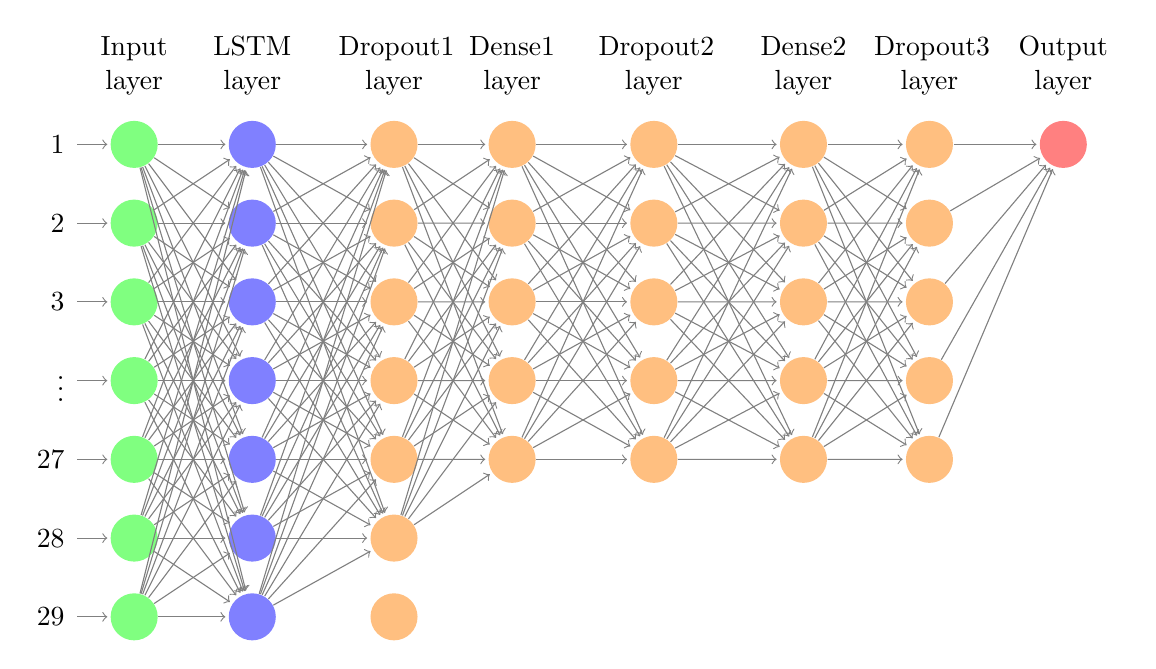
\begin{tikzpicture}[shorten >=1pt,->,draw=black!50, node distance=\layersep]
		\tikzstyle{every pin edge}=[<-,shorten <=1pt]
		\tikzstyle{neuron}=[circle,fill=black!25,minimum size=17pt,inner sep=0pt]
		\tikzstyle{input neuron}=[neuron, fill=green!50];
		\tikzstyle{fase1 neuron}=[neuron, fill=blue!50];
		\tikzstyle{fase2 neuron}=[neuron, fill=orange!50];
		\tikzstyle{output neuron}=[neuron, fill=red!50];
		\tikzstyle{annot} = [text width=4em, text centered]
		
		% Draw the input layer nodes
		\foreach \y in {1,...,7}{
			% This is the same as writing \foreach \name / \y in {1/1,2/2,3/3,4/4}
			\ifnum\y<4
			\node[input neuron, pin=left: \y] (I-\y) at (0,-\y) {};
			\fi
			\ifnum\y=4
			\node[input neuron, pin=left: \vdots] (I-\y) at (0,-\y) {};
			\fi
			\ifnum\y=5
			\node[input neuron, pin=left: 27] (I-\y) at (0,-\y) {};
			\fi
			\ifnum\y=6
			\node[input neuron, pin=left: 28] (I-\y) at (0,-\y) {};
			\fi
			\ifnum\y=7
			\node[input neuron, pin=left: 29] (I-\y) at (0,-\y) {};
			\fi
		}
		
		% Draw the LSTM nodes
		\foreach \y in {1,...,7}
		\node[fase1 neuron, right of=I-4] (H1-\y) at (\layersep*0.5,-\y) {};
		
		% Draw the Dropout_1 nodes
		\foreach \y in {1,...,7}
		\node[fase2 neuron, right of=H1-4] (H2-\y) at (\layersep*2.3,-\y) {};
		
		% Draw the Dense_1 layer nodes
		\foreach \y in {1,...,5}
		\node[fase2 neuron, right of=H2-4] (H3-\y) at (\layersep*3.8,-\y cm) {};
		
		% Draw the Dropout_2 nodes
		\foreach \y in {1,...,5}
		\node[fase2 neuron, right of=H3-3] (H4-\y) at (\layersep*5.6,-\y cm) {};
		
		% Draw the Dense_2 nodes
		\foreach \y in {1,...,5}
		\node[fase2 neuron, right of=H4-3] (H5-\y) at (\layersep*7.5,-\y) {};
		
		% Draw the Dropout_3 layer nodes
		\foreach \y in {1,...,5}
		\node[fase2 neuron, right of=H5-3] (H6-\y) at (\layersep*9.1,-\y cm) {};
		
		% Draw the Dense_3 layer nodes
		\node[output neuron, right of=H6-3] (H7-1) at (\layersep*10.8,-1 cm) {};
		
		% Connect every node in the input layer with every node in the
		% LSTM layer.
		\foreach \source in {1,...,7}
		\foreach \dest in {1,...,7}
		\path (I-\source) edge (H1-\dest);
		% Connect every node in the LSTM layer with every node in the
		% Dropout_1 layer.
		\foreach \source in {1,...,7}
		\foreach \dest in {1,...,6}
		\path (H1-\source) edge (H2-\dest);
		% Connect every node in the Dropout_1 layer with every node in the
		% Dense_1 layer.
		\foreach \source in {1,...,6}
		\foreach \dest in {1,...,5}
		\path (H2-\source) edge (H3-\dest);
		% Connect every node in the Dense_1 layer with every node in the
		% Dropout_2 layer.
		\foreach \source in {1,...,5}
		\foreach \dest in {1,...,5}
		\path (H3-\source) edge (H4-\dest);
		% Connect every node in the Dropout_2 layer with every node in the
		% Dense_2 layer.
		\foreach \source in {1,...,5}
		\foreach \dest in {1,...,5}
		\path (H4-\source) edge (H5-\dest);
		% Connect every node in the Dense_2 layer with every node in the
		% Dropout_3 layer.
		\foreach \source in {1,...,5}
		\foreach \dest in {1,...,5}
		\path (H5-\source) edge (H6-\dest);
		% Connect every node in the Dropout_3 layer with every node in the
		% Dense_3 layer.
		\foreach \source in {1,...,5}
		\path (H6-\source) edge (H7-1);
		
		
		% Annotate the layers
		\node[annot,above of=H1-1, node distance=1cm] {LSTM layer};
		\node[annot,above of=H2-1, node distance=1cm] {Dropout1 layer};
		\node[annot,above of=H3-1, node distance=1cm] {Dense1 layer};
		\node[annot,above of=H4-1, node distance=1cm] {Dropout2 layer};
		\node[annot,above of=H5-1, node distance=1cm] {Dense2 layer};
		\node[annot,above of=H6-1, node distance=1cm] {Dropout3 layer};
		\node[annot,above of=I-1] {Input layer};
		\node[annot,above of=H7-1] {Output layer};
	\end{tikzpicture}
	\caption{Modelo LSTM}
\end{figure}

  Ya concluida la presentaci\'{o}n y fundamentaci\'{o}n del funcionamiento y estructura de los algoritmos de DL a utilizar en el proyecto, es posible proceder a la evaluaci\'{o}n de los algoritmos. La evaluaci\'{o}n y aplicaci\'{o}n del conocimiento forman los pasos finales de la metodolog\'{i}a aplicada para el desarrollo del proyecto. Para la evaluaci\'{o}n de los algoritmos se realizar\'{a}n $7$ experimentos que ser\'{a}n detallados y representados sus resultados en el siguiente cap\'{i}tulo, y finalizando el mismo la aplicaci\'{o}n del conocimiento adquirido.
	\chapter{Evaluaci\'{o}n y aplicaci\'{o}n de los modelos DL}

  Este cap\'{i}tulo abarca la evaluaci\'{o}n de los modelos de DL seleccionados en los pasos anteriores de la metodolog\'{i}a KDD. Para ello est\'{a}n definidas las m\'{e}tricas y algunos par\'{a}metros, no obstante, es necesario realizar unas primeras pruebas para terminar de ajustar los par\'{a}metros restantes. En las tablas obtenidas de los resultados se definen tres colores representativos, que va a permitir definir una superioridad o inferioridad de los algoritmos, estos colores son:
  \begin{itemize}
  	\item \colorbox{green}{Verde}: representa el valor m\'{a}s alto en la m\'{e}trica.
  	\item \colorbox{yellow}{Amarillo}: representa el segundo mejor valor de la m\'{e}trica.
  	\item \colorbox{red}{Rojo}: representa el peor valor de la m\'{e}trica.
  \end{itemize}

Ahora se procede a realizar los experimentos definidos para evaluar los algoritmos propuestos. Estos experimentos conforman la parte $8$ de la metodolog\'{i}a, centrada en la evaluaci\'{o}n de los modelos seleccionados.

\section{Experimento 1: Comparaci\'{o}n entre la selecci\'{o}n de datos para las pruebas}

Este primer experimento est\'{a} basado en buscar la mejor proporci\'{o}n de datos para el entrenamiento y prueba, para ello se usar\'{a} el algoritmo KNN de ML con los datos desbalanceados.

\begin{table}[h!]
	\begin{longtable}{|c|c|c|c|c|c|c|}
		\hline
		\%Test & Model & Accuracy & AUC & Precision& Recall & F1 \\ \hline
		10\% & KNN IMBALANCE & \colorbox{yellow}{0.997} & \colorbox{green}{0.571} & \colorbox{green}{1} & \colorbox{green}{0.14285714} & \colorbox{green}{0.25} \\ \hline
		20\% & KNN IMBALANCE & \colorbox{green}{0.99775} & \colorbox{yellow}{0.55} & \colorbox{green}{1} & \colorbox{yellow}{0.1} & \colorbox{yellow}{0.181818182}\\ \hline
		30\% & KNN IMBALANCE & 0.996833333 & 0.525 & \colorbox{green}{1} & 0.05 & 0.09523809523809523\\ \hline
		40\% & KNN IMBALANCE & \colorbox{red}{0.996375} & \colorbox{red}{0.5} & \colorbox{red}{0} & \colorbox{red}{0} & \colorbox{red}{0}\\ \hline
		50\% & KNN IMBALANCE & 0.9971 & \colorbox{red}{0.5}	& \colorbox{red}{0} & \colorbox{red}{0} & \colorbox{red}{0}\\ \hline
	\end{longtable}
	\caption{Puntuaci\'{o}n de tama\~{n}os de prueba en KNN desbalanceado.}
	\label{t:1}
\end{table}

\begin{figure}[h!]
	\centering
	\includegraphics[width=0.8\textwidth]{"figuras/Experimento1/KNN_Test_size"}
	\caption{Puntuaciones por tama\~{n}os de prueba en KNN desbalanceado.}
\end{figure}

Observaciones:
\begin{enumerate}
	\item Los peores resultados se obtienen cuando el por ciento de datos para la prueba es de 40\% y 50\% del conjunto de datos.
	\item El mejor resultado lo obtiene cuando el por ciento de datos para las pruebas es de un 10\% del conjunto de datos.
	\item La mejor exactitud de predicci\'{o}n es cuando se realiza la prueba con un 20\% del conjunto de datos.
\end{enumerate}

Por lo tanto, se decide tomar un 20\% de datos para realizar las pruebas, porque posee mayor exactitud y posee el segundo mejor resultado de \textit{F1 Score}, ya que con un 10\% se pierde exactitud en las predicciones a pesar de tener el mejor \textit{F1 Score}.

\section{Experimento 2: Comparaci\'{o}n entre los modelos de ML por estrategias para solucionar al desbalance de la informaci\'{o}n}

  El objetivo de este experimento es seleccionar los mejores modelos ML por estrategias. Para ello se utilizar\'{a}n los modelos DT, GNB, KNN, LR, MLP, RF y XGBOOST, y cada modelo se le aplicar\'{a}n las estrategias con datos desbalanceados, UnderSampler, OverSampler, SMOTE y ADASYN. Una vez definido los modelos y estrategias, se procede a realizar el experimento y obtener los resultados.
  
  \begin{longtable}{|c|c|c|c|c|c|}
  	\hline
  	Model & Accuracy & AUC & Precision & Recall & F1\\ \hline
  	\endfirsthead
  	\hline
  	Model & Accuracy & AUC & Precision & Recall & F1\\ \hline
  	\endhead
  	RF IMABALANCED & \colorbox{green}{0.99775} & 0.681567 & \colorbox{yellow}{0.666667} & 0.363636 & \colorbox{green}{0.470588}\\ \hline
  	XGBOOST IMBALANCED & \colorbox{yellow}{0.9975} & 	0.681442 & 0.571429 & 0.363636 & \colorbox{yellow}{0.444444}\\ \hline
  	KNN IMBALANCE & \colorbox{green}{0.99775} & 0.590909 & \colorbox{green}{1} & 0.181818 & 0.307692\\ \hline
  	DT IMBALANCED & 0.99425 & 0.679813 & 0.2 & 0.363636 & 0.258065\\ \hline
  	RF ADASYN & 0.997 & 0.583083 & 0.5 & 0.166667 & 0.25\\ \hline
  	RF OVERSAMPLE & 0.997 & 0.599499 & 0.333333 & 0.2 & 0.25\\ \hline
  	XGBOOST  & 0.9965 & 0.599248 & 0.25 & 0.2 & 0.222222\\ \hline
  	DT OVERSAMPLE & 0.99575 & 0.598872 & 0.181818 & 0.2 & 0.190476\\ \hline
  	RF SMOTE & 0.99675 & 0.535714 & \colorbox{green}{1} & 0.071429 & 0.133333\\ \hline
  	XGBOOST ADASYN  & 0.9925 & 0.580826 & 0.090909 & 0.166667 & 0.117647\\ \hline
  	NB IMBALANCED & 0.98 & \colorbox{green}{0.717997} & 0.063291 & 0.454545 & 0.111111\\ \hline
  	XGBOOST SMOTE & 0.99425 & 0.53446 & 0.090909 & 0.071429 & 0.08\\ \hline
  	LR ADASYN  & 0.986 & 0.577566 & 0.041667 & 0.166667 & 0.066667\\ \hline
  	NB UNDERSAMPLE & 0.96425 & \colorbox{yellow}{0.710101} & 0.035211 & 0.454545 & 0.065359\\ \hline
  	LR SMOTE & 0.98525 & 0.565533 & 0.040816 & 0.142857 & 0.063492\\ \hline
  	LR OVERSAMPLE & 0.9845 & 0.593233 & 0.035714 & 0.2 & 0.060606\\ \hline
  	NB ADASYN & 0.969 & 0.610582 & 0.025424 & 0.25 & 0.046154\\ \hline
  	DT SMOTE & 0.98575 & 0.530195 & 0.022222 & 0.071429 & 0.033898\\ \hline
  	MLP  ADASYN & 0.95275 & 0.602432 & 0.016393 & 0.25 & 0.030769\\ \hline
  	DT ADASYN & 0.9825 & 0.534269 & 0.016667 & 0.083333 & 0.027778\\ \hline
  	NB OVERSAMPLE & 0.96275 & 0.582331 & 0.013986 & 0.2 & 0.026144\\ \hline
  	MLP SMOTE & 0.95575 & 0.550731 & 0.011976 & 0.142857 & 0.022099\\ \hline
  	NB SMOTE & 0.972 & 0.523296 & 0.01 & 0.071429 & 0.017544\\ \hline
  	KNN SMOTE & 0.76225 & 0.595997 & 0.006322 & 0.428571 & 0.012461\\ \hline
  	RF UNDERSAMPLE & 0.724 & 0.634973 & 0.00543 & 0.545455 & 0.010753\\ \hline
  	KNN ADASYN & 0.806 & 0.570378 & 0.005181 & 0.333333 & 0.010204\\ \hline
  	DT UNDERSAMPLE & 0.586 & 0.611112 & 0.004219 & 0.636364 & 0.008383\\ \hline
  	XGBOOST UNDERSAMPLE & 0.32725 & 0.572039 & 0.003336 & \colorbox{green}{0.818182} & 0.006645\\ \hline
  	KNN UNDERSAMPLE & 0.57375 & 0.514312 & 0.002934 & 0.454545 & 0.005831\\ \hline
  	MLP UNDERSAMPLE & 0.03425 & 0.515793 & 0.002839 & \colorbox{green}{1} & 0.005663\\ \hline
  	LR UNDERSAMPLE & \colorbox{red}{0.00275} & 0.5 & 0.00275 & \colorbox{green}{1} & 0.005485\\ \hline
  	MLP OVERSAMPLE & 0.155 & \colorbox{red}{0.376942} & 0.001774 & 0.6 & 0.003538\\ \hline
  	MLP IMBALANCE & 0.99675 & 0.499749 & \colorbox{red}{0} & \colorbox{red}{0} & \colorbox{red}{0}\\ \hline
  	KNN OVERSAMPLE & 0.9915 & 0.496992 & \colorbox{red}{0} & \colorbox{red}{0} & \colorbox{red}{0}\\ \hline
  	LR IMBALANCED & 0.99725 & 0.5 & \colorbox{red}{0} & \colorbox{red}{0} & \colorbox{red}{0}\\ \hline
  	\caption{Puntuaciones de las pruebas de los modelos ML por estrategias.}
  	\label{t:2}
  \end{longtable}

Basados en la tabla \ref{t:2} y en los anexos ~\ref{an:1}, ~\ref{an:2}, ~\ref{an:3}, ~\ref{an:4} y ~\ref{an:5}, se pueden obtener las siguientes observaciones:

\begin{itemize}
	\item El modelo con mejor resultado es RF con datos desbalanceados.
	\item El segundo mejor resultado lo obtiene el modelo XGBOOST con datos desbalanceados.
	\item El peor resultado lo obtiene el modelo LR con datos desbalanceados.
	\item El mejor resultado en el modelo DT se obtiene con la estrategia OverSampler.
	\item El mejor resultado en el modelo KNN se obtiene con los datos desbalanceados.
	\item El mejor resultado en el modelo LR se obtiene con ADASYN.
	\item El mejor resultado en el modelo MPLClssifier se obtiene con ADASYN.
	\item El mejor resultado en el modelo NB se obtiene con datos desbalanceados.
	\item El mejor resultado en el modelo RF se obtiene con datos desbalanceados.
	\item El mejor resultado en el modelo XGBOOST se obtiene con datos desbalanceados.
	\item El mejor resultado con datos desbalanceados lo obtiene el modelo RF.
	\item El mejor resultado con UnderSampler lo obtiene el modelo NB.
	\item El mejor resultado con OverSampler lo obtiene el modelo RF.
	\item El mejor resultado con SMOTE lo obtiene el modelo RF.
	\item El mejor resultado con ADASYN lo obtiene el modelo RF.
	\item El modelo RF presenta superioridad con respecto a los dem\'{a}s modelos.
\end{itemize}

Con estas observaciones son suficientes para decidir los modelos que representar\'{a}n a los modelos ML. Se escoge el modelo RF con datos desbalanceados, OverSampler, SMOTE y ADASYN, y el modelo NB con UnderSampler para pr\'{o}ximos experimentos como los mejores modelos ML.

\section{Experimento 3: Comparaci\'{o}n en el orden de los \textit{dropout} con datos desbalanceados}

En este experimento se analizar\'{a} el orden los \textit{dropout} de los algoritmos CNN y RNN, donde el m\'{a}ximo posible recomendado por la librer\'{i}a es $0.5$. Se realizar\'{a}n las pruebas con datos desbalanceados y $1$ \textit{epoch} para los \'{o}rdenes de \textit{dropout} mostrados en la tabla.

	\begin{longtable}{|c|c|c|c|c|c|c|}
		\hline
		Dropout & Model & Accuracy & AUC & Precision & Recall & F1\\ \hline
		\endfirsthead
		\hline
		Dropout & Model & Accuracy & AUC & Precision & Recall & F1\\ \hline
		\endhead
		0.5-0.4-0.3 & CNN IMBALANCE & \colorbox{green}{0.999} & \colorbox{green}{0.714286} & \colorbox{green}{0.999001} & \colorbox{green}{0.999} & \colorbox{green}{0.9988}\\ \hline
		0.3-0.4-0.5 & CNN IMBALANCE & \colorbox{green}{0.999} & \colorbox{green}{0.714286} & \colorbox{green}{0.999001} & \colorbox{green}{0.999} & \colorbox{green}{0.9988}\\ \hline
		0.5-0.5-0.5 & CNN IMBALANCE & \colorbox{green}{0.999} & \colorbox{green}{0.714286} & \colorbox{green}{0.999001} & \colorbox{green}{0.999} & \colorbox{green}{0.9988}\\ \hline
		0.4-0.4-0.4 & CNN IMBALANCE & \colorbox{yellow}{0.99875} & \colorbox{yellow}{0.71416} & \colorbox{yellow}{0.998563} & \colorbox{yellow}{0.99875} & \colorbox{yellow}{0.99858}\\ \hline
		0.3-0.3-0.3 & CNN IMBALANCE & \colorbox{yellow}{0.99875} & \colorbox{yellow}{0.71416} & \colorbox{yellow}{0.998563} & \colorbox{yellow}{0.99875} & \colorbox{yellow}{0.99858}\\ \hline
		0.2-0.2-0.2 & CNN IMBALANCE & \colorbox{yellow}{0.99875} & \colorbox{yellow}{0.71416} & \colorbox{yellow}{0.998563} & \colorbox{yellow}{0.99875} & \colorbox{yellow}{0.99858}\\ \hline
		0.2-0.2-0.5 & CNN IMBALANCE & \colorbox{yellow}{0.99875} & \colorbox{yellow}{0.71416} & \colorbox{yellow}{0.998563} & \colorbox{yellow}{0.99875} & \colorbox{yellow}{0.99858}\\ \hline
		0.5-0.2-0.2 & CNN IMBALANCE & \colorbox{yellow}{0.99875} & \colorbox{yellow}{0.71416} & \colorbox{yellow}{0.998563} & \colorbox{yellow}{0.99875} & \colorbox{yellow}{0.99858}\\ \hline
		0.5-0.4-0.3 & RNN IMBALANCE & \colorbox{red}{0.99825} & \colorbox{red}{0.5} & \colorbox{red}{0.996503} & \colorbox{red}{0.99825} & \colorbox{red}{0.997376}\\ \hline
		0.3-0.4-0.5 & RNN IMBALANCE & \colorbox{red}{0.99825} & \colorbox{red}{0.5} & \colorbox{red}{0.996503} & \colorbox{red}{0.99825} & \colorbox{red}{0.997376}\\ \hline
		0.5-0.5-0.5 & RNN IMBALANCE & \colorbox{red}{0.99825} & \colorbox{red}{0.5} & \colorbox{red}{0.996503} & \colorbox{red}{0.99825} & \colorbox{red}{0.997376}\\ \hline
		0.4-0.4-0.4 & RNN IMBALANCE & \colorbox{red}{0.99825} & \colorbox{red}{0.5} & \colorbox{red}{0.996503} & \colorbox{red}{0.99825} & \colorbox{red}{0.997376}\\ \hline
		0.3-0.3-0.3 & RNN IMBALANCE & \colorbox{red}{0.99825} & \colorbox{red}{0.5} & \colorbox{red}{0.996503} & \colorbox{red}{0.99825} & \colorbox{red}{0.997376}\\ \hline
		0.2-0.2-0.2 & RNN IMBALANCE & \colorbox{red}{0.99825} & \colorbox{red}{0.5} & \colorbox{red}{0.996503} & \colorbox{red}{0.99825} & \colorbox{red}{0.997376}\\ \hline
		0.2-0.2-0.5 & RNN IMBALANCE & \colorbox{red}{0.99825} & \colorbox{red}{0.5} & \colorbox{red}{0.996503} & \colorbox{red}{0.99825} & \colorbox{red}{0.997376}\\ \hline
		0.5-0.2-0.2 & RNN IMBALANCE & \colorbox{red}{0.99825} & \colorbox{red}{0.5} & \colorbox{red}{0.996503} & \colorbox{red}{0.99825} & \colorbox{red}{0.997376}\\ \hline
		\caption{Puntuaci\'{o}n en las pruebas del modelo CNN con datos desbalanceados para los \'{o}rdenes de \textit{dropout}.}
		\label{t:3}
	\end{longtable}

\begin{figure}[h!]
	\centering
	\includegraphics[width=0.8\textwidth]{"figuras/Experimento3/CNN_dropouts_tests"}
	\caption{Puntuaciones en las pruebas del modelo CNN con datos desbalanceados por dropouts.}
	\label{ff:1}
\end{figure}

\begin{figure}[h!]
	\centering
	\includegraphics[width=0.8\textwidth]{"figuras/Experimento3/RNN_dropouts_tests"}
	\caption{Puntuaciones en las pruebas del modelo RNN con datos desbalanceados por dropouts.}
	\label{ff:2}
\end{figure}

Basados en la tabla \ref{t:3} y en las figuras \ref{ff:1} y \ref{ff:2}, se obtienen las siguientes observaciones generales:
\begin{itemize}
	\item Los mejores resultados se obtienen con CNN con los dropouts 0.5-0.4-0.3, 0.3-0.4-0.5 y 0.5-0.5-0.5.
	\item Los peores resultados se obtienen con RNN, siendo los resultados indistinguibles con cualquier orden de dropout.
	\item El peor resultado con CNN es con los restantes \'{o}rdenes de dropouts, siendo sus resultados iguales.
	\item Los CNN dominan a RNN en cualquier orden de dropout.
\end{itemize}

Teniendo en cuenta esto, se decide usar de entre los 3 mejores dropouts, el orden 0.5-0.4-0.3 para los pr\'{o}ximos experimentos

\section{Experimento 4: Comparaci\'{o}n en los modelos DL teniendo en cuenta los resultados de las pruebas.}

  Este experimento est\'{a} orientado a seleccionar los mejores modelos DL teniendo en cuenta dos factores: la cantidad de \textit{epochs} de entrenamiento y la estrategia aplicada para la soluci\'{o}n al desbalance de la informaci\'{o}n. Para ello este experimento se dividir\'{a} en dos partes: primero, se analizar\'{a}n todos los modelos por \textit{epochs} y con la misma estrategia aplicada, segundo, se analizar\'{a}n todas las estrategias y \textit{epoch} por modelo. Luego de obtener las observaciones por cada una de las dos partes anteriores, se proceder\'{a} a obtener las observaciones generales y junto a ello, los mejores modelos en cuanto a las pruebas.
  
  Para el experimento se tiene en cuenta que: las cantidades de \textit{epochs} son $1$, $20$, $50$ y $100$, las estrategias son datos desbalanceados, UnderSampler, OverSampler, SMOTE y ADASYN, y los modelos a analizar son CNN, AE, DAE, RNN, LSTM y BPNN. Una vez definidas las bases del experimento, se proceden a realizar el experimento y analizarlo por cada una de las partes.

\subsection{Primera parte: Modelos por epochs con la misma estrategia.}

  Los resultados obtenidos se muestran a continuaci\'{o}n, para ello se dividir\'{a} por estrategias:
  
  \subsubsection{Datos desbalanceados}
  	\begin{longtable}{|c|c|c|c|c|c|c|}
  		\hline
  		Epoch & Model & Accuracy & AUC & Precision & Recall & F1\\ \hline
  		\endfirsthead
  		\hline
  		Epoch & Model & Accuracy & AUC & Precision & Recall & F1\\ \hline
  		\endhead
  		1 & CNN IMBALANCE & \colorbox{green}{0.99675} & \colorbox{green}{0.56666667} & \colorbox{green}{0.99676057} & \colorbox{green}{0.99675} & \colorbox{green}{0.99551}\\ \hline
  		50 & CNN IMBALANCE & \colorbox{green}{0.99675} & \colorbox{green}{0.56666667} & \colorbox{green}{0.99676057} & \colorbox{green}{0.99675} & \colorbox{green}{0.99551}\\ \hline
  		20 & CNN IMBALANCE & \colorbox{yellow}{0.9965} & \colorbox{yellow}{0.5665412} & 0.99550976 & \colorbox{yellow}{0.9965} & \colorbox{yellow}{0.99533596}\\ \hline
  		100 & CNN IMBALANCE & \colorbox{red}{0.99625} & 0.56641573 & 0.99488395 & \colorbox{red}{0.99625} & 0.99516706\\ \hline
  		1 & BPNN IMBALANCE & \colorbox{red}{0.99625} & \colorbox{red}{0.5} & \colorbox{yellow}{0.99626406} & \colorbox{red}{0.99625} & \colorbox{red}{0.99437852}\\ \hline
  		20 & BPNN IMBALANCE & \colorbox{red}{0.99625} & \colorbox{red}{0.5} & \colorbox{yellow}{0.99626406} & \colorbox{red}{0.99625} & \colorbox{red}{0.99437852}\\ \hline
  		50 & BPNN IMBALANCE & \colorbox{red}{0.99625} & \colorbox{red}{0.5} & \colorbox{yellow}{0.99626406} & \colorbox{red}{0.99625} & \colorbox{red}{0.99437852}\\ \hline
  		100 & BPNN IMBALANCE & \colorbox{red}{0.99625} & \colorbox{red}{0.5} & \colorbox{yellow}{0.99626406} & \colorbox{red}{0.99625} & \colorbox{red}{0.99437852}\\ \hline
  		1 & AE IMBALANCE & \colorbox{red}{0.99625} & \colorbox{red}{0.5} & \colorbox{red}{0.99251406} & \colorbox{red}{0.99625} & \colorbox{red}{0.99437852}\\ \hline
  		1 & DAE IMBALANCE & \colorbox{red}{0.99625} & \colorbox{red}{0.5} & \colorbox{red}{0.99251406} & \colorbox{red}{0.99625} & \colorbox{red}{0.99437852}\\ \hline
  		1 & RNN IMBALANCE & \colorbox{red}{0.99625} & \colorbox{red}{0.5} & \colorbox{red}{0.99251406} & \colorbox{red}{0.99625} & \colorbox{red}{0.99437852}\\ \hline
  		1 & LSTM IMBALANCE & \colorbox{red}{0.99625} & \colorbox{red}{0.5} & \colorbox{red}{0.99251406} & \colorbox{red}{0.99625} & \colorbox{red}{0.99437852}\\ \hline
  		20 & AE IMBALANCE & \colorbox{red}{0.99625} & \colorbox{red}{0.5} & \colorbox{red}{0.99251406} & \colorbox{red}{0.99625} & \colorbox{red}{0.99437852}\\ \hline
  		20 & DAE IMBALANCE & \colorbox{red}{0.99625} & \colorbox{red}{0.5} & \colorbox{red}{0.99251406} & \colorbox{red}{0.99625} & \colorbox{red}{0.99437852}\\ \hline
  		20 & RNN IMBALANCE & \colorbox{red}{0.99625} & \colorbox{red}{0.5} & \colorbox{red}{0.99251406} & \colorbox{red}{0.99625} & \colorbox{red}{0.99437852}\\ \hline
  		20 & LSTM IMBALANCE & \colorbox{red}{0.99625} & \colorbox{red}{0.5} & \colorbox{red}{0.99251406} & \colorbox{red}{0.99625} & \colorbox{red}{0.99437852}\\ \hline
  		50 & AE IMBALANCE & \colorbox{red}{0.99625} & \colorbox{red}{0.5} & \colorbox{red}{0.99251406} & \colorbox{red}{0.99625} & \colorbox{red}{0.99437852}\\ \hline
  		50 & DAE IMBALANCE & \colorbox{red}{0.99625} & \colorbox{red}{0.5} & \colorbox{red}{0.99251406} & \colorbox{red}{0.99625} & \colorbox{red}{0.99437852}\\ \hline
  		50 & RNN IMBALANCE & \colorbox{red}{0.99625} & \colorbox{red}{0.5} & \colorbox{red}{0.99251406} & \colorbox{red}{0.99625} & \colorbox{red}{0.99437852}\\ \hline
  		50 & LSTM IMBALANCE & \colorbox{red}{0.99625} & \colorbox{red}{0.5} & \colorbox{red}{0.99251406} & \colorbox{red}{0.99625} & \colorbox{red}{0.99437852}\\ \hline
  		100 & AE IMBALANCE & \colorbox{red}{0.99625} & \colorbox{red}{0.5} & \colorbox{red}{0.99251406} & \colorbox{red}{0.99625} & \colorbox{red}{0.99437852}\\ \hline
  		100 & DAE IMBALANCE & \colorbox{red}{0.99625} & \colorbox{red}{0.5} & \colorbox{red}{0.99251406} & \colorbox{red}{0.99625} & \colorbox{red}{0.99437852}\\ \hline
  		100 & RNN IMBALANCE & \colorbox{red}{0.99625} & \colorbox{red}{0.5} & \colorbox{red}{0.99251406} & \colorbox{red}{0.99625} & \colorbox{red}{0.99437852}\\ \hline
  		100 & LSTM IMBALANCE & \colorbox{red}{0.99625} & \colorbox{red}{0.5} & \colorbox{red}{0.99251406} & \colorbox{red}{0.99625} & \colorbox{red}{0.99437852}\\ \hline
  		\caption{Puntuaciones en las pruebas de los modelos DL con datos desbalanceados en 1, 20, 50 y 100 epochs.}
  		\label{t:4}
  	\end{longtable}

Basados en la tabla \ref{t:4} se obitenen las siguientes observaciones:
\begin{itemize}
	\item El mejor modelo es CNN con 1 y 50 \textit{epochs} con los mejores resultados.
	\item El segundo mejor modelo es CNN con 20 \textit{epochs} con los segundos mejores resultados a excepci\'{o}n de la precisi\'{o}n.
	\item Los peores modelos son AE, DAE, RNN y LSTM con los resultados id\'{e}nticos y los peores.
	\item La superioridad de modelos sin tener en cuenta la cantidad de \textit{epochs} es: CNN, BPNN y el resto en tercer lugar.
	\item Los resultados del modelo BPNN se comportas igual sin importar la cantidad de \textit{epochs}.
\end{itemize}

\subsubsection{UnderSampler}
\begin{longtable}{|c|c|c|c|c|c|c|}
	\hline
	Epoch & Model & Accuracy & AUC & Precision & Recall & F1\\ \hline
	\endfirsthead
	\hline
	Epoch & Model & Accuracy & AUC & Precision & Recall & F1\\ \hline
	\endhead
	1 & BPNN UNDERSAMPLE & \colorbox{green}{0.99625} & 0.5 & \colorbox{yellow}{0.99626406} & \colorbox{green}{0.99625} & \colorbox{green}{0.99437852}\\ \hline
	20 & BPNN UNDERSAMPLE & \colorbox{green}{0.99625} & 0.5 & \colorbox{yellow}{0.99626406} & \colorbox{green}{0.99625} & \colorbox{green}{0.99437852}\\ \hline
	50 & BPNN UNDERSAMPLE & \colorbox{green}{0.99625} & 0.5 & \colorbox{yellow}{0.99626406} & \colorbox{green}{0.99625} & \colorbox{green}{0.99437852}\\ \hline
	100 & BPNN UNDERSAMPLE & \colorbox{green}{0.99625} & 0.5 & \colorbox{yellow}{0.99626406} & \colorbox{green}{0.99625} & \colorbox{green}{0.99437852}\\ \hline
	1 & AE UNDERSAMPLE & \colorbox{green}{0.99625} & 0.5 & 0.99251406 & \colorbox{green}{0.99625} & \colorbox{green}{0.99437852}\\ \hline
	1 & DAE UNDERSAMPLE & \colorbox{green}{0.99625} & 0.5 & 0.99251406 & \colorbox{green}{0.99625} & \colorbox{green}{0.99437852}\\ \hline
	1 & RNN UNDERSAMPLE & \colorbox{green}{0.99625} & 0.5 & 0.99251406 & \colorbox{green}{0.99625} & \colorbox{green}{0.99437852}\\ \hline
	1 & LSTM UNDERSAMPLE & \colorbox{green}{0.99625} & 0.5 & 0.99251406 & \colorbox{green}{0.99625} & \colorbox{green}{0.99437852}\\ \hline
	20 & AE UNDERSAMPLE & \colorbox{green}{0.99625} & 0.5 & 0.99251406 & \colorbox{green}{0.99625} & \colorbox{green}{0.99437852}\\ \hline
	20 & DAE UNDERSAMPLE & \colorbox{green}{0.99625} & 0.5 & 0.99251406 & \colorbox{green}{0.99625} & \colorbox{green}{0.99437852}\\ \hline
	20 & RNN UNDERSAMPLE & \colorbox{green}{0.99625} & 0.5 & 0.99251406 & \colorbox{green}{0.99625} & \colorbox{green}{0.99437852}\\ \hline
	20 & LSTM UNDERSAMPLE & \colorbox{green}{0.99625} & 0.5 & 0.99251406 & \colorbox{green}{0.99625} & \colorbox{green}{0.99437852}\\ \hline
	50 & AE UNDERSAMPLE & \colorbox{green}{0.99625} & 0.5 & 0.99251406 & \colorbox{green}{0.99625} & \colorbox{green}{0.99437852}\\ \hline
	50 & DAE UNDERSAMPLE & \colorbox{green}{0.99625} & 0.5 & 0.99251406 & \colorbox{green}{0.99625} & \colorbox{green}{0.99437852}\\ \hline
	50 & RNN UNDERSAMPLE & \colorbox{green}{0.99625} & 0.5 & 0.99251406 & \colorbox{green}{0.99625} & \colorbox{green}{0.99437852}\\ \hline
	50 & LSTM UNDERSAMPLE & \colorbox{green}{0.99625} & 0.5 & 0.99251406 & \colorbox{green}{0.99625} & \colorbox{green}{0.99437852}\\ \hline
	100 & AE UNDERSAMPLE & \colorbox{green}{0.99625} & 0.5 & 0.99251406 & \colorbox{green}{0.99625} & \colorbox{green}{0.99437852}\\ \hline
	100 & DAE UNDERSAMPLE & \colorbox{green}{0.99625} & 0.5 & 0.99251406 & \colorbox{green}{0.99625} & \colorbox{green}{0.99437852}\\ \hline
	100 & RNN UNDERSAMPLE & \colorbox{green}{0.99625} & 0.5 & 0.99251406 & \colorbox{green}{0.99625} & \colorbox{green}{0.99437852}\\ \hline
	100 & LSTM UNDERSAMPLE & \colorbox{green}{0.99625} & 0.5 & 0.99251406 & \colorbox{green}{0.99625} & \colorbox{green}{0.99437852}\\ \hline
	100 & CNN UNDERSAMPLE & \colorbox{yellow}{0.76675} & \colorbox{green}{0.61727311} & 0.99368038 & \colorbox{yellow}{0.76675} & \colorbox{yellow}{0.86451737}\\ \hline
	50 & CNN UNDERSAMPLE & 0.53675 & 0.5350481 & 0.99301653 & 0.53675 & 0.69518094\\ \hline
	20 & CNN UNDERSAMPLE & 0.121 & \colorbox{red}{0.45922208} & \colorbox{red}{0.98997066} & 0.121 & 0.21089089\\ \hline
	1 & CNN UNDERSAMPLE & \colorbox{red}{0.0765} & \colorbox{yellow}{0.53651192} & \colorbox{green}{0.99626517} & \colorbox{red}{0.0765} & \colorbox{red}{0.13562832}\\ \hline
	\caption{Puntuaciones en las pruebas de los modelos DL con UnderSampler en 1, 20, 50 y 100 epochs.}
	\label{t:5}
\end{longtable}

Basados en la tabla \ref{t:5} se obtienen las siguientes observaciones:
\begin{itemize}
	\item El mejor modelo es BPNN en $1$, $20$, $50$ y $100$ con los mejores resultados a excepci\'{o}n de la precisi\'{o}n con los segundos mejores resultados y \textit{AUC Score}.
	\item Los segundos mejores modelos son AE, DAE, RNN y LSTM en $1$, $20$, $50$ y $100$ \textit{epochs} con resultados id\'{e}nticos a BPNN a diferencia de la precisi\'{o}n donde obtiene resultados m\'{a}s bajos.
	\item El peor modelo es CNN con $1$ \textit{epoch} con los peores resultados a excepci\'{o}n de \textit{AUC Score} con el segundo mejor resultado y la precisi\'{o}n con el mejor resultado.
	\item Los modelos AE, DAE, RNN y LSTM no presentan comportamientos diferentes en cuanto a los resultados sin importar el n\'{u}mero de \textit{epochs}.
\end{itemize}

\subsubsection{OverSampler}
\begin{longtable}{|c|c|c|c|c|c|c|}
	\hline
	Epoch & Model & Accuracy & AUC & Precision & Recall & F1\\ \hline
	\endfirsthead
	\hline
	Epoch & Model & Accuracy & AUC & Precision & Recall & F1\\ \hline
	\endhead
	1 & BPNN OVERSAMPLE & \colorbox{green}{0.99575} & \colorbox{red}{0.5} & \colorbox{green}{0.99576806} & \colorbox{green}{0.99575} & \colorbox{green}{0.99362953}\\ \hline
	20 & BPNN OVERSAMPLE & \colorbox{green}{0.99575} & \colorbox{red}{0.5} & \colorbox{green}{0.99576806} & \colorbox{green}{0.99575} & \colorbox{green}{0.99362953}\\ \hline
	50 & BPNN OVERSAMPLE & \colorbox{green}{0.99575} & \colorbox{red}{0.5} & \colorbox{green}{0.99576806} & \colorbox{green}{0.99575} & \colorbox{green}{0.99362953}\\ \hline
	100 & BPNN OVERSAMPLE & \colorbox{green}{0.99575} & \colorbox{red}{0.5} & \colorbox{green}{0.99576806} & \colorbox{green}{0.99575} & \colorbox{green}{0.99362953}\\ \hline
	1 & AE OVERSAMPLE & \colorbox{green}{0.99575} & \colorbox{red}{0.5} & \colorbox{red}{0.99151806} & \colorbox{green}{0.99575} & \colorbox{green}{0.99362953}\\ \hline
	1 & DAE OVERSAMPLE & \colorbox{green}{0.99575} & \colorbox{red}{0.5} & \colorbox{red}{0.99151806} & \colorbox{green}{0.99575} & \colorbox{green}{0.99362953}\\ \hline
	1 & RNN OVERSAMPLE & \colorbox{green}{0.99575} & \colorbox{red}{0.5} & \colorbox{red}{0.99151806} & \colorbox{green}{0.99575} & \colorbox{green}{0.99362953}\\ \hline
	1 & LSTM OVERSAMPLE & \colorbox{green}{0.99575} & \colorbox{red}{0.5} & \colorbox{red}{0.99151806} & \colorbox{green}{0.99575} & \colorbox{green}{0.99362953}\\ \hline
	20 & AE OVERSAMPLE & \colorbox{green}{0.99575} & \colorbox{red}{0.5} & \colorbox{red}{0.99151806} & \colorbox{green}{0.99575} & \colorbox{green}{0.99362953}\\ \hline
	20 & DAE OVERSAMPLE & \colorbox{green}{0.99575} & \colorbox{red}{0.5} & \colorbox{red}{0.99151806} & \colorbox{green}{0.99575} & \colorbox{green}{0.99362953}\\ \hline
	20 & RNN OVERSAMPLE & \colorbox{green}{0.99575} & \colorbox{red}{0.5} & \colorbox{red}{0.99151806} & \colorbox{green}{0.99575} & \colorbox{green}{0.99362953}\\ \hline
	20 & LSTM OVERSAMPLE & \colorbox{green}{0.99575} & \colorbox{red}{0.5} & \colorbox{red}{0.99151806} & \colorbox{green}{0.99575} & \colorbox{green}{0.99362953}\\ \hline
	50 & AE OVERSAMPLE & \colorbox{green}{0.99575} & \colorbox{red}{0.5} & \colorbox{red}{0.99151806} & \colorbox{green}{0.99575} & \colorbox{green}{0.99362953}\\ \hline
	50 & DAE OVERSAMPLE & \colorbox{green}{0.99575} & \colorbox{red}{0.5} & \colorbox{red}{0.99151806} & \colorbox{green}{0.99575} & \colorbox{green}{0.99362953}\\ \hline
	50 & RNN OVERSAMPLE & \colorbox{green}{0.99575} & \colorbox{red}{0.5} & \colorbox{red}{0.99151806} & \colorbox{green}{0.99575} & \colorbox{green}{0.99362953}\\ \hline
	50 & LSTM OVERSAMPLE & \colorbox{green}{0.99575} & \colorbox{red}{0.5} & \colorbox{red}{0.99151806} & \colorbox{green}{0.99575} & \colorbox{green}{0.99362953}\\ \hline
	100 & AE OVERSAMPLE & \colorbox{green}{0.99575} & \colorbox{red}{0.5} & \colorbox{red}{0.99151806} & \colorbox{green}{0.99575} & \colorbox{green}{0.99362953}\\ \hline
	100 & DAE OVERSAMPLE & \colorbox{green}{0.99575} & \colorbox{red}{0.5} & \colorbox{red}{0.99151806} & \colorbox{green}{0.99575} & \colorbox{green}{0.99362953}\\ \hline
	100 & RNN OVERSAMPLE & \colorbox{green}{0.99575} & \colorbox{red}{0.5} & \colorbox{red}{0.99151806} & \colorbox{green}{0.99575} & \colorbox{green}{0.99362953}\\ \hline
	100 & LSTM OVERSAMPLE & \colorbox{green}{0.99575} & \colorbox{red}{0.5} & \colorbox{red}{0.99151806} & \colorbox{green}{0.99575} & \colorbox{green}{0.99362953}\\ \hline
	100 & CNN OVERSAMPLE & \colorbox{yellow}{0.9875} & \colorbox{yellow}{0.70086101} & \colorbox{yellow}{0.99386401} & \colorbox{yellow}{0.9875} & \colorbox{yellow}{0.99040606}\\ \hline
	50 & CNN OVERSAMPLE & 0.9865 & 0.70035888 & 0.99381181 & 0.9865 & 0.98984607\\ \hline
	20 & CNN OVERSAMPLE & 0.98475 & 0.69948014 & 0.99373693 & 0.98475 & 0.98887889\\ \hline
	1 & CNN OVERSAMPLE & \colorbox{red}{0.93125} & \colorbox{green}{0.7019022} & 0.99346889 & \colorbox{red}{0.93125} & \colorbox{red}{0.9604627}\\ \hline
	\caption{Puntuaciones en las pruebas de los modelos DL con OverSampler en 1, 20, 50 y 100 epochs.}
	\label{t:6}
\end{longtable}

Basados en la tabla \ref{t:6} se obitenen las siguietnes observaciones:
\begin{itemize}
	\item El mejor modelo es BPNN en $1$, $20$, $50$ y $100$ \textit{epochs} con resultados id\'{e}nticos y los mejores a excepci\'{o}n de \textit{AUC Score} que obtiene el peor resultado.
	\item Los segundos mejores modelos son AE, DAE, RNN y LSTM con resultados id\'{e}nticos a BPNN a excepci\'{o}n de la precisi\'{o}n donde obtienen los peores resultados.
	\item El peor modelo es CNN en $1$ \textit{epoch} donde obtiene los peores resultados a excepci\'{o}n de \textit{AUC Score} con el mejor resultado y la precisi\'{o}n.
	\item Los resultados de los modelos AE, DAE, RNN y LSTM se comportan iguales sin importar la cantidad de \textit{epochs}.
\end{itemize}

\subsubsection{SMOTE}
\begin{longtable}{|c|c|c|c|c|c|c|}
	\hline
	Epoch & Model & Accuracy & AUC & Precision & Recall & F1\\ \hline
	\endfirsthead
	\hline
	Epoch & Model & Accuracy & AUC & Precision & Recall & F1\\ \hline
	\endhead
	1 & BPNN SMOTE & \colorbox{green}{0.9955} & \colorbox{red}{0.5} & \colorbox{green}{0.99552025} & \colorbox{green}{0.9955} & \colorbox{green}{0.99325507}\\ \hline
	20 & BPNN SMOTE & \colorbox{green}{0.9955} & \colorbox{red}{0.5} & \colorbox{green}{0.99552025} & \colorbox{green}{0.9955} & \colorbox{green}{0.99325507}\\ \hline
	50 & BPNN SMOTE & \colorbox{green}{0.9955} & \colorbox{red}{0.5} & \colorbox{green}{0.99552025} & \colorbox{green}{0.9955} & \colorbox{green}{0.99325507}\\ \hline
	100 & BPNN SMOTE & \colorbox{green}{0.9955} & \colorbox{red}{0.5} & \colorbox{green}{0.99552025} & \colorbox{green}{0.9955} & \colorbox{green}{0.99325507}\\ \hline
	1 & AE SMOTE & \colorbox{green}{0.9955} & \colorbox{red}{0.5} & \colorbox{red}{0.99102025} & \colorbox{green}{0.9955} & \colorbox{green}{0.99325507}\\ \hline
	1 & DAE SMOTE & \colorbox{green}{0.9955} & \colorbox{red}{0.5} & \colorbox{red}{0.99102025} & \colorbox{green}{0.9955} & \colorbox{green}{0.99325507}\\ \hline
	1 & RNN SMOTE & \colorbox{green}{0.9955} & \colorbox{red}{0.5} & \colorbox{red}{0.99102025} & \colorbox{green}{0.9955} & \colorbox{green}{0.99325507}\\ \hline
	1 & LSTM SMOTE & \colorbox{green}{0.9955} & \colorbox{red}{0.5} & \colorbox{red}{0.99102025} & \colorbox{green}{0.9955} & \colorbox{green}{0.99325507}\\ \hline
	20 & AE SMOTE & \colorbox{green}{0.9955} & \colorbox{red}{0.5} & \colorbox{red}{0.99102025} & \colorbox{green}{0.9955} & \colorbox{green}{0.99325507}\\ \hline
	20 & DAE SMOTE & \colorbox{green}{0.9955} & \colorbox{red}{0.5} & \colorbox{red}{0.99102025} & \colorbox{green}{0.9955} & \colorbox{green}{0.99325507}\\ \hline
	20 & RNN SMOTE & \colorbox{green}{0.9955} & \colorbox{red}{0.5} & \colorbox{red}{0.99102025} & \colorbox{green}{0.9955} & \colorbox{green}{0.99325507}\\ \hline
	20 & LSTM SMOTE & \colorbox{green}{0.9955} & \colorbox{red}{0.5} & \colorbox{red}{0.99102025} & \colorbox{green}{0.9955} & \colorbox{green}{0.99325507}\\ \hline
	50 & AE SMOTE & \colorbox{green}{0.9955} & \colorbox{red}{0.5} & \colorbox{red}{0.99102025} & \colorbox{green}{0.9955} & \colorbox{green}{0.99325507}\\ \hline
	50 & DAE SMOTE & \colorbox{green}{0.9955} & \colorbox{red}{0.5} & \colorbox{red}{0.99102025} & \colorbox{green}{0.9955} & \colorbox{green}{0.99325507}\\ \hline
	50 & RNN SMOTE & \colorbox{green}{0.9955} & \colorbox{red}{0.5} & \colorbox{red}{0.99102025} & \colorbox{green}{0.9955} & \colorbox{green}{0.99325507}\\ \hline
	50 & LSTM SMOTE & \colorbox{green}{0.9955} & \colorbox{red}{0.5} & \colorbox{red}{0.99102025} & \colorbox{green}{0.9955} & \colorbox{green}{0.99325507}\\ \hline
	100 & AE SMOTE & \colorbox{green}{0.9955} & \colorbox{red}{0.5} & \colorbox{red}{0.99102025} & \colorbox{green}{0.9955} & \colorbox{green}{0.99325507}\\ \hline
	100 & DAE SMOTE & \colorbox{green}{0.9955} & \colorbox{red}{0.5} & \colorbox{red}{0.99102025} & \colorbox{green}{0.9955} & \colorbox{green}{0.99325507}\\ \hline
	100 & RNN SMOTE & \colorbox{green}{0.9955} & \colorbox{red}{0.5} & \colorbox{red}{0.99102025} & \colorbox{green}{0.9955} & \colorbox{green}{0.99325507}\\ \hline
	100 & LSTM SMOTE & \colorbox{green}{0.9955} & \colorbox{red}{0.5} & \colorbox{red}{0.99102025} & \colorbox{green}{0.9955} & \colorbox{green}{0.99325507}\\ \hline
	50 & CNN SMOTE & \colorbox{yellow}{0.99225} & \colorbox{green}{0.60897651} & \colorbox{yellow}{0.9928545} & \colorbox{yellow}{0.99225} & \colorbox{yellow}{0.99254662}\\ \hline
	100 & CNN SMOTE & 0.99125 & \colorbox{yellow}{0.60847425} & 0.99271384 & 0.99125 & 0.99195836\\ \hline
	20 & CNN SMOTE & 0.98975 & 0.60772085 & 0.99256918 & 0.98975 & 0.99110131\\ \hline
	1 & CNN SMOTE & \colorbox{red}{0.39575} & 0.55824823 & 0.99236381 & \colorbox{red}{0.39575} & \colorbox{red}{0.56255824}\\ \hline
	\caption{Puntuaciones en las pruebas de los modelos DL con SMOTE en 1, 20, 50 y 100 epochs.}
	\label{t:7}
\end{longtable}

Basados en la tabla \ref{t:7} se obtienen las siguietnes observaciones:
\begin{itemize}
	\item El mejor modelo es BPNN en $1$, $20$, $50$ y $100$ \textit{epochs}, con los mejores resultados a excepci\'{o}n del \textit{AUC Score} que obtiene el peor resultado.
	\item Los segundos mejores modelos son AE, DAE, RNN y LSTM con $1$, $20$, $50$ y $100$ \textit{epochs} con resultados id\'{e}nticos a BPNN a excepci\'{o}n de la precisi\'{o}n donde obtienen los peores resultados.
	\item El peor modelo es CNN en $1$ \textit{epoch} con los peores resultados a excepci\'{o}n de \textit{AUC Score} y la precisi\'{o}n.
	\item Los modelos AE, DAE, RNN y LSTM tienen resultados iguales sin importar el n\'{u}mero de \textit{epochs}.
\end{itemize}

\subsubsection{ADASYN}
\begin{longtable}{|c|c|c|c|c|c|c|}
	\hline
	Epoch & Model & Accuracy & AUC & Precision & Recall & F1\\ \hline
	\endfirsthead
	\hline
	Epoch & Model & Accuracy & AUC & Precision & Recall & F1\\ \hline
	\endhead
	1 & BPNN ADASYN & \colorbox{green}{0.99525} & \colorbox{red}{0.5} & \colorbox{green}{0.99527256} & \colorbox{green}{0.99525} & \colorbox{green}{0.99288065}\\ \hline
	20 & BPNN ADASYN & \colorbox{green}{0.99525} & \colorbox{red}{0.5} & \colorbox{green}{0.99527256} & \colorbox{green}{0.99525} & \colorbox{green}{0.99288065}\\ \hline
	50 & BPNN ADASYN & \colorbox{green}{0.99525} & \colorbox{red}{0.5} & \colorbox{green}{0.99527256} & \colorbox{green}{0.99525} & \colorbox{green}{0.99288065}\\ \hline
	100 & BPNN ADASYN & \colorbox{green}{0.99525} & \colorbox{red}{0.5} & \colorbox{green}{0.99527256} & \colorbox{green}{0.99525} & \colorbox{green}{0.99288065}\\ \hline
	1 & AE ADASYN & \colorbox{green}{0.99525} & \colorbox{red}{0.5} & \colorbox{red}{0.99052256} & \colorbox{green}{0.99525} & \colorbox{green}{0.99288065}\\ \hline
	1 & DAE ADASYN & \colorbox{green}{0.99525} & \colorbox{red}{0.5} & \colorbox{red}{0.99052256} & \colorbox{green}{0.99525} & \colorbox{green}{0.99288065}\\ \hline
	1 & RNN ADASYN & \colorbox{green}{0.99525} & \colorbox{red}{0.5} & \colorbox{red}{0.99052256} & \colorbox{green}{0.99525} & \colorbox{green}{0.99288065}\\ \hline
	1 & LSTM ADASYN & \colorbox{green}{0.99525} & \colorbox{red}{0.5} & \colorbox{red}{0.99052256} & \colorbox{green}{0.99525} & \colorbox{green}{0.99288065}\\ \hline
	20 & AE ADASYN & \colorbox{green}{0.99525} & \colorbox{red}{0.5} & \colorbox{red}{0.99052256} & \colorbox{green}{0.99525} & \colorbox{green}{0.99288065}\\ \hline
	20 & DAE ADASYN & \colorbox{green}{0.99525} & \colorbox{red}{0.5} & \colorbox{red}{0.99052256} & \colorbox{green}{0.99525} & \colorbox{green}{0.99288065}\\ \hline
	20 & RNN ADASYN & \colorbox{green}{0.99525} & \colorbox{red}{0.5} & \colorbox{red}{0.99052256} & \colorbox{green}{0.99525} & \colorbox{green}{0.99288065}\\ \hline
	20 & LSTM ADASYN & \colorbox{green}{0.99525} & \colorbox{red}{0.5} & \colorbox{red}{0.99052256} & \colorbox{green}{0.99525} & \colorbox{green}{0.99288065}\\ \hline
	50 & AE ADASYN & \colorbox{green}{0.99525} & \colorbox{red}{0.5} & \colorbox{red}{0.99052256} & \colorbox{green}{0.99525} & \colorbox{green}{0.99288065}\\ \hline
	50 & DAE ADASYN & \colorbox{green}{0.99525} & \colorbox{red}{0.5} & \colorbox{red}{0.99052256} & \colorbox{green}{0.99525} & \colorbox{green}{0.99288065}\\ \hline
	50 & RNN ADASYN & \colorbox{green}{0.99525} & \colorbox{red}{0.5} & \colorbox{red}{0.99052256} & \colorbox{green}{0.99525} & \colorbox{green}{0.99288065}\\ \hline
	50 & LSTM ADASYN & \colorbox{green}{0.99525} & \colorbox{red}{0.5} & \colorbox{red}{0.99052256} & \colorbox{green}{0.99525} & \colorbox{green}{0.99288065}\\ \hline
	100 & AE ADASYN & \colorbox{green}{0.99525} & \colorbox{red}{0.5} & \colorbox{red}{0.99052256} & \colorbox{green}{0.99525} & \colorbox{green}{0.99288065}\\ \hline
	100 & DAE ADASYN & \colorbox{green}{0.99525} & \colorbox{red}{0.5} & \colorbox{red}{0.99052256} & \colorbox{green}{0.99525} & \colorbox{green}{0.99288065}\\ \hline
	100 & RNN ADASYN & \colorbox{green}{0.99525} & \colorbox{red}{0.5} & \colorbox{red}{0.99052256} & \colorbox{green}{0.99525} & \colorbox{green}{0.99288065}\\ \hline
	100 & LSTM ADASYN & \colorbox{green}{0.99525} & \colorbox{red}{0.5} & \colorbox{red}{0.99052256} & \colorbox{green}{0.99525} & \colorbox{green}{0.99288065}\\ \hline
	100 & CNN ADASYN & \colorbox{yellow}{0.99125} & \colorbox{green}{0.62894142} & \colorbox{yellow}{0.9926573} & \colorbox{yellow}{0.99125} & \colorbox{yellow}{0.99192671}\\ \hline
	50 & CNN ADASYN & 0.99 & \colorbox{yellow}{0.62831344} & 0.99250555 & 0.99 & 0.99119245\\ \hline
	20 & CNN ADASYN & 0.97925 & 0.62291278 & 0.62291278 & 0.97925 & 0.98531359\\ \hline
	1 & CNN ADASYN & \colorbox{red}{0.38025} & 0.53150491 & 0.99133065 & \colorbox{red}{0.38025} & \colorbox{red}{0.54630481}\\ \hline
	\caption{Puntuaciones en las pruebas de los modelos DL con ADASYN en 1, 20, 50 y 100 epochs.}
	\label{t:8}
\end{longtable}

Basados en la tabla \ref{t:8} se obtienen las siguientes observaciones:
\begin{itemize}
	\item El mejor modelo es BPNN en $1$, $20$, $50$ y $100$ \textit{epochs}, con los mejores resultados a excepci\'{o}n del \textit{AUC Score} que obtiene el peor resultado.
	\item Los segundos mejores modelos son AE, DAE, RNN y LSTM con $1$, $20$, $50$ y $100$ \textit{epochs} con resultados id\'{e}nticos a BPNN a excepci\'{o}n de la precisi\'{o}n donde obtienen los peores resultados.
	\item El peor modelo es CNN en $1$ \textit{epoch} con los peores resultados a excepci\'{o}n de \textit{AUC Score} y la precisi\'{o}n.
	\item Los modelos AE, DAE, RNN y LSTM tienen resultados iguales sin importar el n\'{u}mero de \textit{epochs}.
\end{itemize}

\subsection{An\'{a}lisis de la primera parte}
  Basados en las comparaciones realizadas en la primera parte se puede llegar a la conclusi\'{o}n de que:
  \begin{itemize}
  	\item Para datos desbalanceados el mejor modelo es CNN, mientras que los dem\'{a}s modelos tienen resultados id\'{e}nticos a pesar de que BPNN tiene la precisi\'{o}n mejor que el resto.
  	\item Para UnderSampler, OverSampler, SMOTE y ADASYN, el mejor modelo es BPNN, aunque posea resultados similares a AE, DAE, RNN y LSTM, este posee mayor precisi\'{o}n en los resultados.
  	\item Por cada estrategia aplicada, los modelos AE, DAE, RNN y LSTM obtienen resultados similares sin importar la cantidad de \textit{epochs}.
  \end{itemize}

  Teniendo en cuenta esto, se decide utilizar para pr\'{o}ximos experimentos el modelo CNN con datos desbalanceados y el modelo BPNN con UnderSampler, OverSampler, SMOTE y ADASYN.

\subsection{Segunda parte: Estrategias y epochs por modelos}

  Con los resultados obtenidos se pueden comparar las estrategias de los modelos por cada \textit{epoch} de forma tal de que se pueda obtener la mejor estrategia y \textit{epoch} por modelo.
  
  \subsubsection{CNN}
  \begin{longtable}{|c|c|c|c|c|c|c|}
  	\hline
  	Epoch & Model & Accuracy & AUC & Precision & Recall & F1\\ \hline
  	\endfirsthead
  	\hline
  	Epoch & Model & Accuracy & AUC & Precision & Recall & F1\\ \hline
  	\endhead
  	50 & CNN IMBALANCE & \colorbox{green}{0.99675} & 0.56666667 & \colorbox{green}{0.99676057} & \colorbox{green}{0.99675} & \colorbox{green}{0.99551}\\ \hline
  	1 & CNN IMBALANCE & \colorbox{green}{0.99675} & 0.56666667 & \colorbox{green}{0.99676057} & \colorbox{green}{0.99675} & \colorbox{green}{0.99551}\\ \hline
  	20 & CNN IMBALANCE & \colorbox{yellow}{0.9965} & 0.5665412 & 0.99550976 & \colorbox{yellow}{0.9965} & \colorbox{yellow}{0.99533596}\\ \hline
  	100 & CNN IMBALANCE & 0.99625 & 0.56641573 & 0.99488395 & 0.99625 & 0.99516706\\ \hline
  	50 & CNN SMOTE & 0.99225 & 0.60897651 & 0.9928545 & 0.99225 & 0.99254662\\ \hline
  	100 & CNN SMOTE & 0.99125 & 0.60847425 & 0.99271384 & 0.99125 & 0.99195836\\ \hline
  	100 & CNN ADASYN & 0.99125 & 0.62894142 & 0.9926573 & 0.99125 & 0.99192671\\ \hline
  	50 & CNN ADASYN & 0.99 & 0.62831344 & 0.99250555 & 0.99 & 0.99119245\\ \hline
  	20 & CNN SMOTE & 0.98975 & 0.60772085 & 0.99256918 & 0.98975 & 0.99110131\\ \hline
  	100 & CNN OVERSAMPLE & 0.9875 & \colorbox{green}{0.70086101} & 0.99386401 & 0.9875 & 0.99040606\\ \hline
  	50 & CNN OVERSAMPLE & 0.9865 & \colorbox{yellow}{0.70035888} & 0.99381181 & 0.9865 & 0.98984607\\ \hline
  	20 & CNN OVERSAMPLE & 0.98475 & 0.69948014 & 0.99373693 & 0.98475 & 0.98887889\\ \hline
  	20 & CNN ADASYN & 0.97925 & 0.62291278 & 0.99202191 & 0.97925 & 0.98531359\\ \hline
  	1 & CNN OVERSAMPLE & 0.93125 & 0.7019022 & 0.99346889 & 0.93125 & 0.9604627\\ \hline
  	100 & CNN UNDERSAMPLE & 0.76675 & 0.61727311 & 0.99368038 & 0.76675 & 0.86451737\\ \hline
  	50 & CNN UNDERSAMPLE & 0.53675 & 0.5350481 & 0.99301653 & 0.53675 & 0.69518094\\ \hline
  	1 & CNN SMOTE & 0.39575 & 0.55824823 & 0.99236381 & 0.39575 & 0.56255824\\ \hline
  	1 & CNN ADASYN & 0.38025 & 0.53150491 & 0.99133065 & 0.38025 & 0.54630481\\ \hline
  	20 & CNN UNDERSAMPLE & 0.121 & \colorbox{red}{0.45922208} & \colorbox{red}{0.98997066} & 0.121 & 0.21089089\\ \hline
  	1 & CNN UNDERSAMPLE & \colorbox{red}{0.0765} & 0.53651192 & \colorbox{yellow}{0.99626517} & \colorbox{red}{0.0765} & \colorbox{red}{0.13562832}\\ \hline
  	\caption{Puntuaciones en las pruebas del modelo CNN por estrategias en 1, 20, 50 y 100 epochs.}
  	\label{t:9}
  \end{longtable}

Basados en la tabla \ref{t:9} se obtienen las siguientes observaciones:
\begin{itemize}
	\item La mejor estrategia es con datos desbalanceados en $1$ y $50$ \textit{epochs} con resultados id\'{e}nticos.
	\item La segunda mejor estrategia es con datos desbalanceados en $20$ \textit{epochs}.
	\item La peor estrategia es UnderSampler en $1$ \textit{epoch}.
	\item El orden de las tres mejores estrategias sin tener en cuenta la cantidad de \textit{epochs} es: datos desbalanceados, SMOTE y ADASYN.
	\item El mejor resultado del modelo CNN con datos desbalanceados se obtiene en $1$ y $50$ \textit{epochs}.
	\item El mejor resultado del modelo CNN con UnderSampler, OverSampler y ADASYN se obtiene en $100$ \textit{epochs}.
	\item El mejor resultado del modelo CNN con SMOTE se obtiene en $50$ \textit{epochs}.
\end{itemize}

\subsubsection{AE}
\begin{longtable}{|c|c|c|c|c|c|c|}
	\hline
	Epoch & Model & Accuracy & AUC & Precision & Recall & F1\\ \hline
	\endfirsthead
	\hline
	Epoch & Model & Accuracy & AUC & Precision & Recall & F1\\ \hline
	\endhead
	20 & AE UNDERSAMPLE & \colorbox{green}{0.99625} & 0.5 & \colorbox{green}{0.992514} & \colorbox{green}{0.99625} & \colorbox{green}{0.994379}\\ \hline
	1 & AE IMBALANCE & \colorbox{green}{0.99625} & 0.5 & \colorbox{green}{0.992514} & \colorbox{green}{0.99625} & \colorbox{green}{0.994379}\\ \hline
	50 & AE UNDERSAMPLE & \colorbox{green}{0.99625} & 0.5 & \colorbox{green}{0.992514} & \colorbox{green}{0.99625} & \colorbox{green}{0.994379}\\ \hline
	100 & AE IMBALANCE & \colorbox{green}{0.99625} & 0.5 & \colorbox{green}{0.992514} & \colorbox{green}{0.99625} & \colorbox{green}{0.994379}\\ \hline
	100 & AE UNDERSAMPLE & \colorbox{green}{0.99625} & 0.5 & \colorbox{green}{0.992514} & \colorbox{green}{0.99625} & \colorbox{green}{0.994379}\\ \hline
	50 & AE IMBALANCE & \colorbox{green}{0.99625} & 0.5 & \colorbox{green}{0.992514} & \colorbox{green}{0.99625} & \colorbox{green}{0.994379}\\ \hline
	1 & AE UNDERSAMPLE & \colorbox{green}{0.99625} & 0.5 & \colorbox{green}{0.992514} & \colorbox{green}{0.99625} & \colorbox{green}{0.994379}\\ \hline
	20 & AE IMBALANCE & \colorbox{green}{0.99625} & 0.5 & \colorbox{green}{0.992514} & \colorbox{green}{0.99625} & \colorbox{green}{0.994379}\\ \hline
	100 & AE OVERSAMPLE & \colorbox{yellow}{0.99575} & 0.5 & \colorbox{yellow}{0.991518} & \colorbox{yellow}{0.99575} & \colorbox{yellow}{0.99363}\\ \hline
	1 & AE OVERSAMPLE & \colorbox{yellow}{0.99575} & 0.5 & \colorbox{yellow}{0.991518} & \colorbox{yellow}{0.99575} & \colorbox{yellow}{0.99363}\\ \hline
	50 & AE OVERSAMPLE & \colorbox{yellow}{0.99575} & 0.5 & \colorbox{yellow}{0.991518} & \colorbox{yellow}{0.99575} & \colorbox{yellow}{0.99363}\\ \hline
	20 & AE OVERSAMPLE & \colorbox{yellow}{0.99575} & 0.5 & \colorbox{yellow}{0.991518} & \colorbox{yellow}{0.99575} & \colorbox{yellow}{0.99363}\\ \hline
	100 & AE SMOTE & 0.9955 & 0.5 & 0.99102 & 0.9955 & 0.993255\\ \hline
	20 & AE SMOTE & 0.9955 & 0.5 & 0.99102 & 0.9955 & 0.993255\\ \hline
	50 & AE SMOTE & 0.9955 & 0.5 & 0.99102 & 0.9955 & 0.993255\\ \hline
	1 & AE SMOTE & 0.9955 & 0.5 & 0.99102 & 0.9955 & 0.993255\\ \hline
	100 & AE ADASYN & \colorbox{red}{0.99525} & 0.5 & \colorbox{red}{0.990523} & \colorbox{red}{0.99525} & \colorbox{red}{0.992881}\\ \hline
	1 & AE ADASYN & \colorbox{red}{0.99525} & 0.5 & \colorbox{red}{0.990523} & \colorbox{red}{0.99525} & \colorbox{red}{0.992881}\\ \hline
	50 & AE ADASYN & \colorbox{red}{0.99525} & 0.5 & \colorbox{red}{0.990523} & \colorbox{red}{0.99525} & \colorbox{red}{0.992881}\\ \hline
	20 & AE ADASYN & \colorbox{red}{0.99525} & 0.5 & \colorbox{red}{0.990523} & \colorbox{red}{0.99525} & \colorbox{red}{0.992881}\\ \hline
	\caption{Puntuaciones en las pruebas del modelo AE por estrategias en 1, 20, 50 y 100 epochs.}
	\label{t:10}
\end{longtable}

Basados en la tabla \ref{t:10} se obtienen las siguientes observaciones:
\begin{itemize}
	\item Las mejores estrategias son con datos desbalanceados y UnderSampler sin importar la cantidad de \textit{epochs}.
	\item La segunda mejor estrategia es con OverSampler sin importar la cantidad de \textit{epochs}.
	\item La peor estrategia es con ADASYN sin importar la cantidad de \textit{epochs}.
	\item La cantidad de \textit{epochs} son irrelevantes en cuanto a los resultados obtenidos por estrategias.
\end{itemize}

Teniendo en cuenta los resultados se pueden obtener las mismas observaciones en los modelos DAE, RNN, LSTM y BPNN, aunque los resultados difieren \'{u}nicamente en la precisi\'{o}n en el modelo BPNN donde es mayor. Los resultados para $20$, $50$ y $100$ \textit{epochs} siguen el mismo comportamiento y se pueden obtener los mismos resultados.

Se puede apreciar que los resultados son indiferentes al n\'{u}mero de \textit{epochs}, por lo tanto, para el modelo AE se puede utilizar cualquier cantidad de \textit{epochs}, ya que se obtienen los mismos resultados. De forma similar ocurre con los modelos DAE, RNN, LSTM y BPNN, obteniendo los mismos resultados y observaciones a excepci\'{o}n de BPNN donde los resultados de precisi\'{o}n son mejores.

\subsection{An\'{a}lisis de la segunda parte}
  Las comparaciones anteriores y los resultados expuestos en el anexo \ref{an:6} permiten la obtenci\'{o}n de las siguientes observaciones en general:
  
  \begin{itemize}
  	\item La mejor estrategia para el modelo CNN es con datos desbalanceados en $1$ y $50$ \textit{epochs} con los mejores resultados.
  	\item Las mejores estrategias para los modelos AE, DAE, RNN, LSTM y BPNN son con datos desbalanceados y UnderSampler sin importar la cantidad de \textit{epochs}.
  	\item La peor estrategia para el modelo CNN es con UnderSampler en $1$ \textit{epoch}.
  	\item La peor estrategia en los modelos AE; DAE, RNN, LSTM y BPNN es con ADASYN sin importar la cantidad de \textit{epochs}.
  	\item Los mejores resultados del modelo CNN con datos desbalanceados se obtienen en $1$ y $50$ \textit{epochs}, mientras que con UnderSampler, OverSampler y SMOTE se obtienen en $100$ \textit{epochs} y con SMOTE en $50$ \textit{epochs}.
  	\item Para los modelos a excepci\'{o}n de CNN, no se aprecian diferencias en los resultados sin importar la cantidad de \textit{epochs}, es decir, los resultados se mantienen constantes sin importar el n\'{u}mero de \textit{epochs}.
  \end{itemize}

  Teniendo en cuenta estas observaciones, se decide utilizar el modelo CNN con datos desbalanceados en $1$ y $50$ \textit{epochs}, con OverSampler y ADASYN en $100$ \textit{epochs}, con SMOTE en $50$ \textit{epochs}, y los modelos AE; DAE; RNN, LSTM y BPNN con cualquier estrategia y n\'{u}mero de \textit{epochs} para pr\'{o}ximos experimentos.

\subsection{An\'{a}lisis general del experimento 4}
  Para una mayor comprensi\'{o}n de los resultados y observaciones obtenidas, se obtiene la siguiente matriz de los mejores modelos por estrategias y la cantidad de \textit{epochs} donde obtienen mejores resultados:
  
\begin{longtable}{|c|c|c|c|c|c|}
	\hline
	\multicolumn{6}{|c|}{Estrategias}\\ \hline
	\space & Imbalanced & UnderSampler & OverSampler & SMOTE & ADASYN\\ \hline
	\endfirsthead
	\hline
	\space & Imbalanced & UnderSampler & OverSampler & SMOTE & ADASYN\\ \hline
	\endhead
	CNN & 1 y 50 & - & - & - & -\\ \hline
	AE & - & - & - & - & -\\ \hline
	DAE & - & - & - & - & -\\ \hline
	RNN & - & - & - & - & -\\ \hline
	LSTM & - & - & - & - & -\\ \hline
	BPNN & - & 100 & 100 & 100 & 100\\ \hline
	\caption{Mejores modelos DL por estrategia.}
	\label{t:11}
\end{longtable}

  Teniendo en cuenta la matriz anterior, los mejores modelos son CNN con datos desbalanceados en $1$ y $50$ \textit{epochs}, y el modelo BPNN con UnderSampler, OverSampler, SMOTE y ADASYN en $100$ \textit{epochs}.
  
  \section{Experimento 5: Comparaci\'{o}n de los modelos DL teniendo en cuenta los resultados del entrenamiento}

  Para encontrar de otra posible diferencia entre los modelos, se realiza este experimento que se realiza de conjunto con el experimento 4. En este caso el objetivo es, al igual que en el anterior, seleccionar los mejores modelo DL teniendo en cuenta los mismos factores, pero la gran diferencia es que se centra en el entrenamiento sin tener en cuenta las pruebas. Por ello, el experimento se divide de igual manera en dos partes y concluir\'{a} con la obtenci\'{o}n de los mejores modelos en cuanto al entrenamiento.
  
  Para el experimento se tiene en cuenta las cantidades $1$, $20$, $50$ y $100$ de \textit{epochs}, las estrategias datos desbalanceados, UnderSampler, OverSampler, SMOTE y ADASYN, y los modelos a comparar son CNN, AE, DAE, RNN, LSTM y BPNN. Ahora se procede a obtener los resultados de los entrenamientos y sus comparaciones en cada una de las partes.
  
  \subsection{Primera parte: Modelos por epochs con la misma estrategia}

  El resultado que se espera de esta parte es el mejor modelo por estrategia en cada uno de los \textit{epochs}. Los resultados y observaciones obtenidas se muestran a continuaci\'{o}n.
  
  \subsubsection{Datos desbalanceados}
  \begin{longtable}{|c|c|c|c|c|c|}
  	\hline
  	Epoch & Model & Accuracy & Precision Train & Recall Train & F1 Train\\ \hline
  	\endfirsthead
  	\hline
  	Epoch & Model & Accuracy & Precision Train & Recall Train & F1 Train\\ \hline
  	\endhead
  	100 & CNN IMBALANCE & \colorbox{green}{0.998749971} & \colorbox{green}{0.17832166} & \colorbox{green}{0.17016315} & \colorbox{green}{0.17132866}\\ \hline
  	50 & CNN IMBALANCE & 0.998187482 & \colorbox{yellow}{0.146853134} & \colorbox{yellow}{0.12820512} & \colorbox{yellow}{0.13403264}\\ \hline
  	20 & CNN IMBALANCE & 0.997562528 & 0.1048951 & 0.08974358 & 0.09440558\\ \hline
  	100 & BPNN IMBALANCE & \colorbox{yellow}{0.998687506} & 0.057999995 & 0.057 & 0.05733333\\ \hline
  	50 & BPNN IMBALANCE & 0.998437524 & 0.045999996 & 0.046 & 0.046\\ \hline
  	20 & BPNN IMBALANCE & 0.99849999 & 0.045999996 & 0.044 & 0.04466666\\ \hline
  	1 & CNN IMBALANCE & 0.98724997 & 0.040209785 & 0.04079254 & 0.04009324\\ \hline
  	50 & LSTM IMBALANCE & 0.9979375 & 0.031999998 & 0.032 & 0.032\\ \hline
  	100 & LSTM IMBALANCE & 0.99781251 & 0.029999997 & 0.027 & 0.028\\ \hline
  	100 & RNN IMBALANCE & 0.997437477 & 0.021999998 & 0.02 & 0.02066666\\ \hline
  	20 & LSTM IMBALANCE & 0.997562528 & 0.019999998 & 0.02 & 0.02\\ \hline
  	20 & RNN IMBALANCE & 0.997500002 & 0.017999997 & 0.017 & 0.01733333\\ \hline
  	1 & RNN IMBALANCE & \colorbox{red}{0.968625009} & 0.009999999 & 0.01 & 0.01\\ \hline
  	50 & RNN IMBALANCE & 0.99712503 & 0.007999999 & 0.007 & 0.00733333\\ \hline
  	1 & LSTM IMBALANCE & 0.99150002 & 0.004 & 0.004 & 0.004\\ \hline
  	100 & AE IMBALANCE & 0.996937513 & \colorbox{red}{0} & \colorbox{red}{0} & \colorbox{red}{0}\\ \hline
  	100 & DAE IMBALANCE & 0.996937513 & \colorbox{red}{0} & \colorbox{red}{0} & \colorbox{red}{0}\\ \hline
  	50 & AE IMBALANCE & 0.996937513 & \colorbox{red}{0} & \colorbox{red}{0} & \colorbox{red}{0}\\ \hline
  	50 & DAE IMBALANCE & 0.996937513 & \colorbox{red}{0} & \colorbox{red}{0} & \colorbox{red}{0}\\ \hline
  	20 & AE IMBALANCE & 0.996937513 & \colorbox{red}{0} & \colorbox{red}{0} & \colorbox{red}{0}\\ \hline
  	20 & DAE IMBALANCE & 0.996937513 & \colorbox{red}{0} & \colorbox{red}{0} & \colorbox{red}{0}\\ \hline
  	1 & DAE IMBALANCE & 0.994937479 & \colorbox{red}{0} & \colorbox{red}{0} & \colorbox{red}{0}\\ \hline
  	1 & BPNN IMBALANCE & 0.991937518 & \colorbox{red}{0} & \colorbox{red}{0} & \colorbox{red}{0}\\ \hline
  	1 & AE IMBALANCE & 0.98862499 & \colorbox{red}{0} & \colorbox{red}{0} & \colorbox{red}{0}\\ \hline
  	\caption{Puntuaciones del entrenamiento de los modelos DL con datos desbalanceados en 1, 20, 50 y 100 epochs.}
  	\label{t:12}
  \end{longtable}

  Basados en la tabla \ref{t:12} y los anexos \ref{an:7}, \ref{an:8}, \ref{an:9} y \ref{an:10}, se pueden obtener las siguientes observaciones:
  \begin{itemize}
  	\item El mejor modelo es CNN.
  	\item El segundo mejor modelo es BPNN.
  	\item Los peores modelos son AE y DAE.
  	\item Los modelos CNN y BPNN mejoran sus resultados a medida que aumenta la cantidad de \textit{epochs}.
  	\item Los modelos AE y DAE no mejoran en ninguna cantidad de \textit{epochs}, obteniendo p\'{e}simos resultados.
  \end{itemize}

\subsubsection{UnderSampler}
\begin{longtable}{|c|c|c|c|c|c|}
	\hline
	Epoch & Model & Accuracy & Precision Train & Recall Train & F1 Train\\ \hline
	\endfirsthead
	\hline
	Epoch & Model & Accuracy & Precision Train & Recall Train & F1 Train\\ \hline
	\endhead
	100 & CNN UNDERSAMPLE & \colorbox{green}{0.908163249} & \colorbox{yellow}{0.976190448} & \colorbox{yellow}{0.83673471} & \colorbox{green}{0.90109885}\\ \hline
	100 & BPNN UNDERSAMPLE & 0.816326559 & 0.94155848 & 0.76789212 & \colorbox{yellow}{0.84010977}\\ \hline
	50 & CNN UNDERSAMPLE & \colorbox{yellow}{0.846938789} & 0.886363626 & 0.79591835 & 0.83870965\\ \hline
	20 & CNN UNDERSAMPLE & 0.795918345 & 0.808510661 & 0.77551019 & 0.79166663\\ \hline
	100 & AE UNDERSAMPLE & \colorbox{red}{0.5} & 0.6171875 & \colorbox{green}{1} & 0.73930478\\ \hline
	50 & LSTM UNDERSAMPLE & 0.632653058 & 0.774999976 & 0.58002269 & 0.6529811\\ \hline
	50 & BPNN UNDERSAMPLE & 0.744897962 & \colorbox{green}{1} & 0.48214287 & 0.64673036\\ \hline
	20 & AE UNDERSAMPLE & \colorbox{red}{0.5} & 0.623205423 & 0.80570173 & 0.64404374\\ \hline
	20 & LSTM UNDERSAMPLE & 0.571428597 & 0.667714715 & 0.58994222 & 0.6053344\\ \hline
	1 & AE UNDERSAMPLE & 0.53061223 & 0.632142842 & 0.70472753 & 0.5985378\\ \hline
	100 & LSTM UNDERSAMPLE & 0.622448981 & 0.75 & 0.48333335 & 0.57905978\\ \hline
	1 & CNN UNDERSAMPLE & 0.520408154 & 0.516666651 & 0.63265306 & 0.5688073\\ \hline
	100 & RNN UNDERSAMPLE & 0.765306115 & 0.586779475 & 0.54345655 & 0.56374556\\ \hline
	20 & DAE UNDERSAMPLE & \colorbox{red}{0.5} & 0.3828125 & 0.75 & 0.50680268\\ \hline
	50 & AE UNDERSAMPLE & \colorbox{red}{0.5} & 0.3828125 & 0.75 & 0.50511503\\ \hline
	50 & RNN UNDERSAMPLE & 0.663265288 & 0.52136755 & 0.4696545 & 0.49259257\\ \hline
	20 & RNN UNDERSAMPLE & 0.653061211 & 0.525990665 & 0.40697944 & 0.45634919\\ \hline
	20 & BPNN UNDERSAMPLE & 0.602040827 & 0.446018875 & 0.4627451 & 0.44985989\\ \hline
	1 & RNN UNDERSAMPLE & 0.602040827 & 0.448525131 & 0.430668 & 0.43900132\\ \hline
	1 & LSTM UNDERSAMPLE & 0.520408154 & 0.397058845 & 0.3821016 & 0.38839284\\ \hline
	1 & BPNN UNDERSAMPLE & 0.540816307 & 0.4375 & 0.21666667 & 0.28929761\\ \hline
	1 & DAE UNDERSAMPLE & 0.561224461 & 0.15625 & 0.25 & 0.19230768\\ \hline
	100 & DAE UNDERSAMPLE & 0.5 & \colorbox{red}{0} & \colorbox{red}{0} & \colorbox{red}{0}\\ \hline
	50 & DAE UNDERSAMPLE & 0.5 & \colorbox{red}{0} & \colorbox{red}{0} & \colorbox{red}{0}\\ \hline
	\caption{Puntuaciones del entrenamiento de los modelos DL con UnderSampler en 1, 20, 50 y 100 epochs.}
	\label{t:13}
\end{longtable}

Basados en la tabla \ref{t:13} y los anexos \ref{an:11}, \ref{an:12}, \ref{an:13} y \ref{an:14}, se obtienen las siguientes observaciones:
\begin{itemize}
	\item El mejor modelo es CNN.
	\item El segundo mejor modelo es BPNN.
	\item El peor modelo es DAE.
	\item Los modelos DAE con epochs superiores a los 20, empeoran sus resultados de entrenamiento.
	\item Los modelos CNN y BPNN mejoran sus resultados a medida que aumenta la cantidad de \textit{epochs}.	
\end{itemize}

\subsubsection{OverSampler}
\begin{longtable}{|c|c|c|c|c|c|}
	\hline
	Epoch & Model & Accuracy & Precision Train & Recall Train & F1 Train\\ \hline
	\endfirsthead
	\hline
	Epoch & Model & Accuracy & Precision Train & Recall Train & F1 Train\\ \hline
	\endhead
	100 & BPNN OVERSAMPLE & \colorbox{green}{0.996364295} & \colorbox{green}{0.993416727} & \colorbox{green}{0.99922538} & \colorbox{green}{0.99617994}\\ \hline
	100 & CNN OVERSAMPLE & \colorbox{yellow}{0.993919611} & 0.99008745 & 0.99774992 & \colorbox{yellow}{0.99383694}\\ \hline
	100 & LSTM OVERSAMPLE & 0.993449509 & \colorbox{yellow}{0.99035269} & 0.99682218 & 0.99335557\\ \hline
	50 & BPNN OVERSAMPLE & 0.993042052 & 0.98695153 & \colorbox{yellow}{0.99906373} & 0.99273348\\ \hline
	50 & CNN OVERSAMPLE & 0.991412282 & 0.986423314 & 0.99655753 & 0.99138087\\ \hline
	50 & LSTM OVERSAMPLE & 0.990942121 & 0.985821307 & 0.99627328 & 0.99069422\\ \hline
	20 & CNN OVERSAMPLE & 0.990283966 & 0.985048652 & 0.9956938 & 0.99025965\\ \hline
	100 & RNN OVERSAMPLE & 0.984266281 & 0.978752553 & 0.98808312 & 0.98288071\\ \hline
	20 & LSTM OVERSAMPLE & 0.983200669 & 0.97532773 & 0.9914127 & 0.98272848\\ \hline
	20 & BPNN OVERSAMPLE & 0.982417107 & 0.991747379 & 0.97327888 & 0.98179853\\ \hline
	50 & RNN OVERSAMPLE & 0.982103705 & 0.977232516 & 0.98553199 & 0.98072463\\ \hline
	20 & RNN OVERSAMPLE & 0.979220212 & 0.973606467 & 0.9855867 & 0.97885162\\ \hline
	1 & BPNN OVERSAMPLE & 0.83090955 & 0.83434689 & 0.83071715 & 0.8243857\\ \hline
	1 & CNN OVERSAMPLE & 0.826960444 & 0.825432777 & 0.82687044 & 0.82379562\\ \hline
	1 & RNN OVERSAMPLE & 0.686234593 & 0.686507225 & 0.681256 & 0.67567873\\ \hline
	1 & LSTM OVERSAMPLE & 0.590108454 & 0.666488409 & 0.3947688 & 0.47518793\\ \hline
	20 & AE OVERSAMPLE & 0.500156701 & 0.313696891 & 0.62725449 & 0.41537589\\ \hline
	50 & DAE OVERSAMPLE & \colorbox{red}{0.49316743} & 0.286667079 & 0.58016032 & 0.38089424\\ \hline
	100 & AE OVERSAMPLE & 0.497712016 & 0.23843208 & 0.47645834 & 0.31496578\\ \hline
	1 & AE OVERSAMPLE & 0.494609177 & 0.235250413 & 0.4743332 & 0.31219319\\ \hline
	100 & DAE OVERSAMPLE & 0.498620957 & 0.230783135 & 0.46292585 & 0.30592763\\ \hline
	1 & DAE OVERSAMPLE & 0.49880901 & 0.212330908 & 0.4258517 & 0.28140163\\ \hline
	50 & AE OVERSAMPLE & 0.495612115 & 0.192697898 & 0.38977957 & 0.2556991\\ \hline
	20 & DAE OVERSAMPLE & 0.500438809 & \colorbox{red}{0.149486467} & \colorbox{red}{0.2975952} & \colorbox{red}{0.19771725}\\ \hline
	\caption{Puntuaciones del entrenamiento de los modelos DL con OverSampler en 1, 20, 50 y 100 epochs.}
	\label{t:14}
\end{longtable}

Basados en la tabla \ref{t:14} y los anexos \ref{an:15}, \ref{an:16}, \ref{an:17} y \ref{an:18}, se pueden obtener las siguientes observaciones:
\begin{itemize}
	\item El mejor modelo es BPNN.
	\item El segundo mejor modelo es CNN.
	\item El peor modelo es DAE.
	\item Los modelos CNN, BPNN, RNN y LSTM mejoran sus resultados mientras mayor sea la cantidad de \textit{epochs}.
\end{itemize}

\subsubsection{SMOTE}
\begin{longtable}{|c|c|c|c|c|c|}
	\hline
	Epoch & Model & Accuracy & Precision Train & Recall Train & F1 Train\\ \hline
	\endfirsthead
	\hline
	Epoch & Model & Accuracy & Precision Train & Recall Train & F1 Train\\ \hline
	\endhead
	100 & BPNN SMOTE & \colorbox{green}{0.998997092} & \colorbox{green}{0.998539507} & \colorbox{green}{0.99923921} & \colorbox{green}{0.99884498}\\ \hline
	50 & BPNN SMOTE & \colorbox{yellow}{0.998558342} & \colorbox{yellow}{0.998017848} & \colorbox{yellow}{0.99916291} & \colorbox{yellow}{0.99854267}\\ \hline
	100 & LSTM SMOTE & 0.997524142 & 0.996127367 & 0.99886996 & 0.99741119\\ \hline
	100 & CNN SMOTE & 0.995518386 & 0.994039357 & 0.99706334 & 0.99551123\\ \hline
	50 & CNN SMOTE & 0.993575275 & 0.992109418 & 0.99509072 & 0.99353939\\ \hline
	20 & CNN SMOTE & 0.99069196 & 0.988459527 & 0.99304038 & 0.99065036\\ \hline
	50 & LSTM SMOTE & 0.990880013 & 0.986309826 & 0.99564129 & 0.99063724\\ \hline
	100 & RNN SMOTE & 0.984831393 & 0.981499672 & 0.98868603 & 0.98457217\\ \hline
	50 & RNN SMOTE & 0.984392643 & 0.982494891 & 0.98650694 & 0.98391545\\ \hline
	20 & RNN SMOTE & 0.973047495 & 0.966816664 & 0.97994155 & 0.97239929\\ \hline
	20 & LSTM SMOTE & 0.963958859 & 0.947134852 & 0.9833923 & 0.96373844\\ \hline
	20 & BPNN SMOTE & 0.938291311 & 0.953579187 & 0.92108405 & 0.93480515\\ \hline
	1 & CNN SMOTE & 0.85335964 & 0.859778166 & 0.84736043 & 0.85067493\\ \hline
	1 & BPNN SMOTE & 0.800081491 & 0.81560123 & 0.79757857 & 0.79251993\\ \hline
	1 & RNN SMOTE & 0.719788134 & 0.720076799 & 0.72189444 & 0.71296543\\ \hline
	100 & DAE SMOTE & 0.495800436 & 0.417240739 & 0.83867735 & 0.55287749\\ \hline
	1 & LSTM SMOTE & 0.627648234 & 0.69548589 & 0.48815134 & 0.55267763\\ \hline
	50 & AE SMOTE & 0.501065552 & 0.31172353 & 0.58127224 & 0.396272\\ \hline
	100 & AE SMOTE & 0.498746395 & 0.275425851 & 0.55210423 & 0.36485434\\ \hline
	50 & DAE SMOTE & 0.497868866 & 0.272701651 & 0.54709417 & 0.36141822\\ \hline
	1 & AE SMOTE & 0.501190901 & 0.330650508 & 0.50685281 & 0.35451099\\ \hline
	20 & DAE SMOTE & \colorbox{red}{0.494045377} & 0.1691508 & 0.34468937 & 0.22527717\\ \hline
	20 & AE SMOTE & 0.500407398 & 0.217240199 & 0.25200582 & 0.1867536\\ \hline
	1 & DAE SMOTE & 0.50162971 & \colorbox{red}{0.109249748} & \colorbox{red}{0.21643287} & \colorbox{red}{0.14415723}\\ \hline
	\caption{Puntuaciones del entrenamiento de los modelos DL con SMOTE en 1, 20, 50 y 100 epochs.}
	\label{t:15}
\end{longtable}

Basados en la tabla \ref{t:15} y los anexos \ref{an:19}, \ref{an:20}, \ref{an:21} y \ref{an:22}, se pueden obtener las siguientes observaciones:
\begin{itemize}
	\item El mejor modelo es BPNN.
	\item El segundo mejor modelo es LSTM.
	\item El peor modelo es DAE.
	\item Los modelos CNN, BPNN, RNN, LSTM y DAE mejoran a medida que aumenta la cantidad de \textit{epochs}.
\end{itemize}

\subsubsection{ADASYN}
\begin{longtable}{|c|c|c|c|c|c|}
	\hline
	Epoch & Model & Accuracy & Precision Train & Recall Train & F1 Train\\ \hline
	\endfirsthead
	\hline
	Epoch & Model & Accuracy & Precision Train & Recall Train & F1 Train\\ \hline
	\endhead
	100 & BPNN ADASYN & \colorbox{green}{0.997366965} & \colorbox{green}{0.997244418} & \colorbox{green}{0.99752074} & \colorbox{green}{0.99728757}\\ \hline
	20 & BPNN ADASYN & \colorbox{yellow}{0.996583283} & \colorbox{yellow}{0.996061802} & 0.99714017 & \colorbox{yellow}{0.99647945}\\ \hline
	100 & LSTM ADASYN & 0.996144414 & 0.99491775 & 0.99749511 & 0.99607491\\ \hline
	50 & BPNN ADASYN & 0.995141387 & 0.992640615 & \colorbox{yellow}{0.99756128} & 0.9949252\\ \hline
	100 & CNN ADASYN & 0.993354678 & 0.991527438 & 0.9952265 & 0.99330389\\ \hline
	50 & CNN ADASYN & 0.992288888 & 0.989902735 & 0.99474478 & 0.99225354\\ \hline
	50 & LSTM ADASYN & 0.991285801 & 0.988178194 & 0.99448264 & 0.99104667\\ \hline
	20 & CNN ADASYN & 0.988527358 & 0.985117078 & 0.99214935 & 0.98851031\\ \hline
	100 & RNN ADASYN & 0.98570621 & 0.98420471 & 0.98729259 & 0.9852491\\ \hline
	50 & RNN ADASYN & 0.980973005 & 0.97678107 & 0.98526347 & 0.98037964\\ \hline
	20 & RNN ADASYN & 0.976459146 & 0.971780539 & 0.98173946 & 0.9758895\\ \hline
	20 & LSTM ADASYN & 0.970378041 & 0.961096585 & 0.98171395 & 0.97024137\\ \hline
	1 & CNN ADASYN & 0.865149498 & 0.865566611 & 0.86654222 & 0.86335516\\ \hline
	1 & BPNN ADASYN & 0.771581709 & 0.790596604 & 0.76459557 & 0.76627654\\ \hline
	1 & RNN ADASYN & 0.709234536 & 0.711095929 & 0.70515919 & 0.69940358\\ \hline
	1 & LSTM ADASYN & 0.621904612 & 0.670764625 & 0.49858537 & 0.55402362\\ \hline
	100 & AE ADASYN & 0.501786709 & 0.353379697 & 0.70511532 & 0.4674027\\ \hline
	50 & AE ADASYN & 0.497366935 & 0.333625883 & 0.67001003 & 0.44187346\\ \hline
	50 & DAE ADASYN & 0.495674253 & 0.325257033 & 0.65496492 & 0.4315089\\ \hline
	20 & DAE ADASYN & 0.496489257 & 0.290057659 & 0.58375126 & 0.38466439\\ \hline
	1 & AE ADASYN & 0.499686539 & 0.439912975 & 0.32745457 & 0.2894938\\ \hline
	1 & DAE ADASYN & \colorbox{red}{0.495580226} & 0.112566531 & 0.22968906 & 0.14997599\\ \hline
	100 & DAE ADASYN & 0.497931153 & 0.103723668 & 0.20962888 & 0.13783602\\ \hline
	20 & AE ADASYN & 0.499435782 & \colorbox{red}{0.05381979} & \colorbox{red}{0.10832497} & \colorbox{red}{0.07135723}\\ \hline
	\caption{Puntuaciones del entrenamiento de los modelos DL con ADASYN en 1, 20, 50 y 100 epochs.}
	\label{t:16}
\end{longtable}

Basados en la tabla \ref{t:16} y los anexos \ref{an:23}, \ref{an:24}, \ref{an:25} y \ref{an:26}, se pueden obtener las siguientes observaciones:
\begin{itemize}
	\item El mejor modelo es BPNN.
	\item El segundo mejor modelo es LSTM.
	\item El peor modelo es DAE.
	\item Los modelos CNN, BPNN, RNN, LSTM y DAE mejoran a medida que aumenta la cantidad de \textit{epochs}.
\end{itemize}

\subsection{An\'{a}lisis de la primera parte}

  Por los resultados obtenidos y las observaciones que se han podido apreciar, se pueden obtener las siguientes conclusiones:
  \begin{itemize}
  	\item El mejor modelo en el entrenamiento con datos desbalanceados y UnderSampler es CNN, seguido de BPNN como el segundo mejor modelo en ambas estrategias.
  	\item El mejor modelo en el entrenamiento con OverSampler, SMOTE y ADASYN es BPNN.
  	\item Los modelos BPNN, CNN, RNN y LSTM mejoran sus resultados a medida que aumenta la cantidad de \textit{epochs} en cualquier estrategia aplicada.
  	\item Los peores modelos en todas las estrategias son AE y DAE.
  \end{itemize}

  Basado en las observaciones de la primera parte, se decide tomar el modelo CNN con datos desbalanceados y UnderSampler, y el modelo BPNN con OverSampler, SMOTE y ADASYN para pr\'{o}ximos experimentos.

\subsection{Segunda parte: Estrategias y epochs por modelos}

  Se cambia la forma de comparar los resultados, de forma tal que se obtenga la mejor estrategia y \textit{epoch} por modelo.
  
  \subsubsection{CNN}
  \begin{longtable}{|c|c|c|c|c|c|}
  	\hline
  	Epoch & Model & Accuracy & Precision Train & Recall Train & F1 Train\\ \hline
  	\endfirsthead
  	\hline
  	Epoch & Model & Accuracy & Precision Train & Recall Train & F1 Train\\ \hline
  	\endhead
  	100 & CNN SMOTE & 0.995518386 & \colorbox{green}{0.994039357} & \colorbox{yellow}{0.99706334} & \colorbox{green}{0.99551123}\\ \hline
  	100 & CNN OVERSAMPLE & 0.993919611 & 0.99008745 & \colorbox{green}{0.99774992} & \colorbox{yellow}{0.99383694}\\ \hline
  	50 & CNN SMOTE & 0.993575275 & \colorbox{yellow}{0.992109418} & 0.99509072 & 0.99353939\\ \hline
  	100 & CNN ADASYN & 0.993354678 & 0.991527438 & 0.9952265 & 0.99330389\\ \hline
  	50 & CNN ADASYN & 0.992288888 & 0.989902735 & 0.99474478 & 0.99225354\\ \hline
  	50 & CNN OVERSAMPLE & 0.991412282 & 0.986423314 & 0.99655753 & 0.99138087\\ \hline
  	20 & CNN SMOTE & 0.99069196 & 0.988459527 & 0.99304038 & 0.99065036\\ \hline
  	20 & CNN OVERSAMPLE & 0.990283966 & 0.985048652 & 0.9956938 & 0.99025965\\ \hline
  	20 & CNN ADASYN & 0.988527358 & 0.985117078 & 0.99214935 & 0.98851031\\ \hline
  	100 & CNN UNDERSAMPLE & 0.908163249 & 0.976190448 & 0.83673471 & 0.90109885\\ \hline
  	1 & CNN ADASYN & 0.865149498 & 0.865566611 & 0.86654222 & 0.86335516\\ \hline
  	1 & CNN SMOTE & 0.85335964 & 0.859778166 & 0.84736043 & 0.85067493\\ \hline
  	50 & CNN UNDERSAMPLE & 0.846938789 & 0.886363626 & 0.79591835 & 0.83870965\\ \hline
  	1 & CNN OVERSAMPLE & 0.826960444 & 0.825432777 & 0.82687044 & 0.82379562\\ \hline
  	20 & CNN UNDERSAMPLE & 0.795918345 & 0.808510661 & 0.77551019 & 0.79166663\\ \hline
  	1 & CNN UNDERSAMPLE & \colorbox{red}{0.520408154} & 0.516666651 & 0.63265306 & 0.5688073\\ \hline
  	100 & CNN IMBALANCE & \colorbox{green}{0.998749971} & 0.17832166 & 0.17016315 & 0.17132866\\ \hline
  	50 & CNN IMBALANCE & \colorbox{yellow}{0.998187482} & 0.146853134 & 0.12820512 & 0.13403264\\ \hline
  	20 & CNN IMBALANCE & 0.997562528 & 0.1048951 & 0.08974358 & 0.09440558\\ \hline
  	1 & CNN IMBALANCE & 0.98724997 & \colorbox{red}{0.040209785} & \colorbox{red}{0.04079254} & \colorbox{red}{0.04009324}\\ \hline
  	\caption{Puntuaciones del entrenamiento del modelo CNN por estrategias en 1, 20, 50 y 100 epochs.}
  	\label{t:17}
  \end{longtable}

Basados en la tabla \ref{t:17} y los anexos \ref{an:27}, \ref{an:28}, \ref{an:29} y \ref{an:30} se pueden obtener las siguientes observaciones:
\begin{itemize}
	\item La mejor estrategia es SMOTE en 100 \textit{epochs}.
	\item La segunda mejor estrategia es OverSampler en 100 \textit{epochs}.
	\item La peor estrategia es con datos desbalanceados con 1 \textit{epochs}.
	\item Los resultados del entrenamiento para el modelo CNN en todas las estrategias, mejoran a medida que aumenta la cantidad de \textit{epochs}.
\end{itemize}

\subsubsection{AE}
\begin{longtable}{|c|c|c|c|c|c|}
	\hline
	Epoch & Model & Accuracy & Precision Train & Recall Train & F1 Train\\ \hline
	\endfirsthead
	\hline
	Epoch & Model & Accuracy & Precision Train & Recall Train & F1 Train\\ \hline
	\endhead
	100 & AE UNDERSAMPLE & 0.5 & 0.6171875 & \colorbox{green}{1} & \colorbox{green}{0.73930478}\\ \hline
	20 & AE UNDERSAMPLE & 0.5 & \colorbox{yellow}{0.623205423} & \colorbox{yellow}{0.80570173} & \colorbox{yellow}{0.64404374}\\ \hline
	1 & AE UNDERSAMPLE & 0.53061223 & \colorbox{green}{0.632142842} & 0.70472753 & 0.5985378\\ \hline
	50 & AE UNDERSAMPLE & 0.5 & 0.3828125 & 0.75 & 0.50511503\\ \hline
	100 & AE ADASYN & 0.501786709 & 0.353379697 & 0.70511532 & 0.4674027\\ \hline
	50 & AE ADASYN & 0.497366935 & 0.333625883 & 0.67001003 & 0.44187346\\ \hline
	20 & AE OVERSAMPLE & 0.500156701 & 0.313696891 & 0.62725449 & 0.41537589\\ \hline
	50 & AE SMOTE & 0.501065552 & 0.31172353 & 0.58127224 & 0.396272\\ \hline
	100 & AE SMOTE & 0.498746395 & 0.275425851 & 0.55210423 & 0.36485434\\ \hline
	1 & AE SMOTE & 0.501190901 & 0.330650508 & 0.50685281 & 0.35451099\\ \hline
	100 & AE OVERSAMPLE & \colorbox{red}{0.497712016} & 0.23843208 & 0.47645834 & 0.31496578\\ \hline
	1 & AE OVERSAMPLE & 0.494609177 & 0.235250413 & 0.4743332 & 0.31219319\\ \hline
	1 & AE ADASYN & 0.499686539 & 0.439912975 & 0.32745457 & 0.2894938\\ \hline
	50 & AE OVERSAMPLE & 0.495612115 & 0.192697898 & 0.38977957 & 0.2556991\\ \hline
	20 & AE SMOTE & 0.500407398 & 0.217240199 & 0.25200582 & 0.1867536\\ \hline
	20 & AE ADASYN & 0.499435782 & 0.05381979 & 0.10832497 & 0.07135723\\ \hline
	100 & AE IMBALANCE & \colorbox{green}{0.996937513} & \colorbox{red}{0} & \colorbox{red}{0} & \colorbox{red}{0}\\ \hline
	20 & AE IMBALANCE & \colorbox{green}{0.996937513} & \colorbox{red}{0} & \colorbox{red}{0} & \colorbox{red}{0}\\ \hline
	50 & AE IMBALANCE & \colorbox{green}{0.996937513} & \colorbox{red}{0} & \colorbox{red}{0} & \colorbox{red}{0}\\ \hline
	1 & AE IMBALANCE & \colorbox{yellow}{0.98862499} & \colorbox{red}{0} & \colorbox{red}{0} & \colorbox{red}{0}\\ \hline
	\caption{Puntuaciones del entrenamiento del modelo AE por estrategias en 1, 20, 50 y 100 epochs.}
	\label{t:18}
\end{longtable}

Basados en la tabla \ref{t:18} y los anexos \ref{an:31}, \ref{an:32}, \ref{an:33} y \ref{an:34}, se obtienen las siguientes observaciones:
\begin{itemize}
	\item La mejor estrategia es UnderSampler en 100 \textit{epochs}.
	\item La segunda mejor estrategia es ADASYN en 100 \textit{epochs}.
	\item La peor estrategia es con datos desbalanceados en 1 \textit{epochs}.
	\item Los entrenamientos del modelo AE para las estrategias UnderSampler, OverSampler, SMOTE y ADASYN son inestables.
\end{itemize}

\subsubsection{DAE}
\begin{longtable}{|c|c|c|c|c|c|}
	\hline
	Epoch & Model & Accuracy & Precision Train & Recall Train & F1 Train\\ \hline
	\endfirsthead
	\hline
	Epoch & Model & Accuracy & Precision Train & Recall Train & F1 Train\\ \hline
	\endhead
	100 & DAE SMOTE & 0.495800436 & \colorbox{green}{0.417240739} & \colorbox{green}{0.83867735} & \colorbox{green}{0.55287749}\\ \hline
	20 & DAE UNDERSAMPLE & 0.5 & \colorbox{yellow}{0.3828125} & \colorbox{yellow}{0.75} & \colorbox{yellow}{0.50680268}\\ \hline
	50 & DAE ADASYN & 0.495674253 & 0.325257033 & 0.65496492 & 0.4315089\\ \hline
	20 & DAE ADASYN & 0.496489257 & 0.290057659 & 0.58375126 & 0.38466439\\ \hline
	50 & DAE OVERSAMPLE & \colorbox{red}{0.49316743} & 0.286667079 & 0.58016032 & 0.38089424\\ \hline
	50 & DAE SMOTE & 0.497868866 & 0.272701651 & 0.54709417 & 0.36141822\\ \hline
	100 & DAE OVERSAMPLE & 0.498620957 & 0.230783135 & 0.46292585 & 0.30592763\\ \hline
	1 & DAE OVERSAMPLE & 0.49880901 & 0.212330908 & 0.4258517 & 0.28140163\\ \hline
	20 & DAE SMOTE & 0.494045377 & 0.1691508 & 0.34468937 & 0.22527717\\ \hline
	20 & DAE OVERSAMPLE & 0.500438809 & 0.149486467 & 0.2975952 & 0.19771725\\ \hline
	1 & DAE UNDERSAMPLE & 0.561224461 & 0.15625 & 0.25 & 0.19230768\\ \hline
	1 & DAE ADASYN & 0.495580226 & 0.112566531 & 0.22968906 & 0.14997599\\ \hline
	1 & DAE SMOTE & 0.50162971 & 0.109249748 & 0.21643287 & 0.14415723\\ \hline
	100 & DAE ADASYN & 0.497931153 & 0.103723668 & 0.20962888 & 0.13783602\\ \hline
	20 & DAE IMBALANCE & \colorbox{green}{0.996937513} & \colorbox{red}{0} & \colorbox{red}{0} & \colorbox{red}{0}\\ \hline
	50 & DAE IMBALANCE & \colorbox{green}{0.996937513} & \colorbox{red}{0} & \colorbox{red}{0} & \colorbox{red}{0}\\ \hline
	100 & DAE IMBALANCE & \colorbox{green}{0.996937513} & \colorbox{red}{0} & \colorbox{red}{0} & \colorbox{red}{0}\\ \hline
	1 & DAE IMBALANCE & \colorbox{yellow}{0.994937479} & \colorbox{red}{0} & \colorbox{red}{0} & \colorbox{red}{0}\\ \hline
	50 & DAE UNDERSAMPLE & 0.5 & \colorbox{red}{0} & \colorbox{red}{0} & \colorbox{red}{0}\\ \hline
	100 & DAE UNDERSAMPLE & 0.5 & \colorbox{red}{0} & \colorbox{red}{0} & \colorbox{red}{0}\\ \hline
	\caption{Puntuaciones del entrenamiento del modelo DAE por estrategias en 1, 20, 50 y 100 epochs.}
	\label{t:19}
\end{longtable}

Basados en la tabla \ref{t:19} y los anexos \ref{an:35}, \ref{an:36}, \ref{an:37} y \ref{an:38}, se obtienen las siguientes observaciones:
\begin{itemize}
	\item La mejor estrategia es SMOTE en 100 \textit{epochs}.
	\item La segunda mejor estrategia es UnderSampler en 20 \textit{epochs}.
	\item Las peores estrategias son UnderSampler en 50 y 100 \textit{epochs}, y con datos desbalanceados.
	\item Los entrenamientos del modelo DAE son inestables para todas las estrategias aplicadas.
\end{itemize}

\subsubsection{RNN}
\begin{longtable}{|c|c|c|c|c|c|}
	\hline
	Epoch & Model & Accuracy & Precision Train & Recall Train & F1 Train\\ \hline
	\endfirsthead
	\hline
	Epoch & Model & Accuracy & Precision Train & Recall Train & F1 Train\\ \hline
	\endhead
	100 & RNN ADASYN & 0.98570621 & \colorbox{green}{0.98420471} & 0.98729259 & \colorbox{green}{0.9852491}\\ \hline
	100 & RNN SMOTE & 0.984831393 & 0.981499672 & \colorbox{green}{0.98868603} & \colorbox{yellow}{0.98457217}\\ \hline
	50 & RNN SMOTE & 0.984392643 & \colorbox{yellow}{0.982494891} & 0.98650694 & 0.98391545\\ \hline
	100 & RNN OVERSAMPLE & 0.984266281 & 0.978752553 & \colorbox{yellow}{0.98808312} & 0.98288071\\ \hline
	50 & RNN OVERSAMPLE & 0.982103705 & 0.977232516 & 0.98553199 & 0.98072463\\ \hline
	50 & RNN ADASYN & 0.980973005 & 0.97678107 & 0.98526347 & 0.98037964\\ \hline
	20 & RNN OVERSAMPLE & 0.979220212 & 0.973606467 & 0.9855867 & 0.97885162\\ \hline
	20 & RNN ADASYN & 0.976459146 & 0.971780539 & 0.98173946 & 0.9758895\\ \hline
	20 & RNN SMOTE & 0.973047495 & 0.966816664 & 0.97994155 & 0.97239929\\ \hline
	1 & RNN SMOTE & 0.719788134 & 0.720076799 & 0.72189444 & 0.71296543\\ \hline
	1 & RNN ADASYN & 0.709234536 & 0.711095929 & 0.70515919 & 0.69940358\\ \hline
	1 & RNN OVERSAMPLE & 0.686234593 & 0.686507225 & 0.681256 & 0.67567873\\ \hline
	100 & RNN UNDERSAMPLE & 0.765306115 & 0.586779475 & 0.54345655 & 0.56374556\\ \hline
	50 & RNN UNDERSAMPLE & 0.663265288 & 0.52136755 & 0.4696545 & 0.49259257\\ \hline
	20 & RNN UNDERSAMPLE & 0.653061211 & 0.525990665 & 0.40697944 & 0.45634919\\ \hline
	1 & RNN UNDERSAMPLE & \colorbox{red}{0.602040827} & 0.448525131 & 0.430668 & 0.43900132\\ \hline
	100 & RNN IMBALANCE & \colorbox{yellow}{0.997437477} & 0.021999998 & 0.02 & 0.02066666\\ \hline
	20 & RNN IMBALANCE & \colorbox{green}{0.997500002} & 0.017999997 & 0.017 & 0.01733333\\ \hline
	1 & RNN IMBALANCE & 0.968625009 & 0.009999999 & 0.01 & 0.01\\ \hline
	50 & RNN IMBALANCE & 0.99712503 & \colorbox{red}{0.007999999} & \colorbox{red}{0.007} & \colorbox{red}{0.00733333}\\ \hline
	\caption{Puntuaciones del entrenamiento del modelo RNN por estrategias en 1, 20, 50 y 100 epochs.}
	\label{t:20}
\end{longtable}

Basados en la tabla \ref{t:20} y los anexos \ref{an:39}, \ref{an:40}, \ref{an:41} y \ref{an:42}, se obtienen las siguientes observaciones:
\begin{itemize}
	\item La mejor estrategia es ADASYN en 100 \textit{epochs}.
	\item La segunda mejor estrategia es SMOTE en 100 \textit{epochs}.
	\item La peor estrategia es con datos desbalanceados en 50 \textit{epochs}.
	\item El modelo RNN con las estrategias UnderSampler, OverSampler, SMOTE y ADASYN obtienen mejores resultados en el entrenamiento a medida que aumenta la cantidad de \textit{epochs}, adem\'{a}s presenta estabilidad en los entrenamientos.
\end{itemize}

\subsubsection{LSTM}
\begin{longtable}{|c|c|c|c|c|c|}
	\hline
	Epoch & Model & Accuracy & Precision Train & Recall Train & F1 Train\\ \hline
	\endfirsthead
	\hline
	Epoch & Model & Accuracy & Precision Train & Recall Train & F1 Train\\ \hline
	\endhead
	100 & LSTM SMOTE & 0.997524142 & \colorbox{green}{0.996127367} & \colorbox{green}{0.99886996} & \colorbox{green}{0.99741119}\\ \hline
	100 & LSTM ADASYN & 0.996144414 & \colorbox{yellow}{0.99491775} & \colorbox{yellow}{0.99749511} & \colorbox{yellow}{0.99607491}\\ \hline
	100 & LSTM OVERSAMPLE & 0.993449509 & 0.99035269 & 0.99682218 & 0.99335557\\ \hline
	50 & LSTM ADASYN & 0.991285801 & 0.988178194 & 0.99448264 & 0.99104667\\ \hline
	50 & LSTM OVERSAMPLE & 0.990942121 & 0.985821307 & 0.99627328 & 0.99069422\\ \hline
	50 & LSTM SMOTE & 0.990880013 & 0.986309826 & 0.99564129 & 0.99063724\\ \hline
	20 & LSTM OVERSAMPLE & 0.983200669 & 0.97532773 & 0.9914127 & 0.98272848\\ \hline
	20 & LSTM ADASYN & 0.970378041 & 0.961096585 & 0.98171395 & 0.97024137\\ \hline
	20 & LSTM SMOTE & 0.963958859 & 0.947134852 & 0.9833923 & 0.96373844\\ \hline
	50 & LSTM UNDERSAMPLE & 0.632653058 & 0.774999976 & 0.58002269 & 0.6529811\\ \hline
	20 & LSTM UNDERSAMPLE & 0.571428597 & 0.667714715 & 0.58994222 & 0.6053344\\ \hline
	100 & LSTM UNDERSAMPLE & 0.622448981 & 0.75 & 0.48333335 & 0.57905978\\ \hline
	1 & LSTM ADASYN & 0.621904612 & 0.670764625 & 0.49858537 & 0.55402362\\ \hline
	1 & LSTM SMOTE & 0.627648234 & 0.69548589 & 0.48815134 & 0.55267763\\ \hline
	1 & LSTM OVERSAMPLE & 0.590108454 & 0.666488409 & 0.3947688 & 0.47518793\\ \hline
	1 & LSTM UNDERSAMPLE & \colorbox{red}{0.520408154} & 0.397058845 & 0.3821016 & 0.38839284\\ \hline
	50 & LSTM IMBALANCE & \colorbox{green}{0.9979375} & 0.031999998 & 0.032 & 0.032\\ \hline
	100 & LSTM IMBALANCE & \colorbox{yellow}{0.99781251} & 0.029999997 & 0.027 & 0.028\\ \hline
	20 & LSTM IMBALANCE & 0.997562528 & 0.019999998 & 0.02 & 0.02\\ \hline
	1 & LSTM IMBALANCE & 0.99150002 & \colorbox{red}{0.004} & \colorbox{red}{0.004} & \colorbox{red}{0.004}\\ \hline
	\caption{Puntuaciones del entrenamiento del modelo LSTM por estrategias en 1, 20, 50 y 100 epochs.}
	\label{t:21}
\end{longtable}

Basados en la tabla \ref{t:21} y los anexos \ref{an:43}, \ref{an:44}, \ref{an:45} y \ref{an:46}, se obtienen las siguientes observaciones:
\begin{itemize}
	\item La mejor estrategia es SMOTE en 100 \textit{epochs}.
	\item La segunda mejor estrategia es ADASYN en 100 \textit{epochs}.
	\item La peor estrategia es con datos desbalanceados en 1 \textit{epochs}.
	\item El modelo LSTM con las estrategias SMOTE, ADASYN y OverSampler obtienen mejores resultados a medida que aumenta la cantidad de \textit{epochs}, adem\'{a}s presentan entrenamientos estables.
\end{itemize}

\subsubsection{BPNN}
\begin{longtable}{|c|c|c|c|c|c|}
	\hline
	Epoch & Model & Accuracy & Precision Train & Recall Train & F1 Train\\ \hline
	\endfirsthead
	\hline
	Epoch & Model & Accuracy & Precision Train & Recall Train & F1 Train\\ \hline
	\endhead
	100 & BPNN SMOTE & \colorbox{green}{0.998997092} & 0.998539507 & \colorbox{green}{0.99923921} & \colorbox{green}{0.99884498}\\ \hline
	50 & BPNN SMOTE & 0.998558342 & 0.998017848 & \colorbox{yellow}{0.99916291} & \colorbox{yellow}{0.99854267}\\ \hline
	100 & BPNN ADASYN & 0.997366965 & 0.997244418 & 0.99752074 & 0.99728757\\ \hline
	20 & BPNN ADASYN & 0.996583283 & 0.996061802 & 0.99714017 & 0.99647945\\ \hline
	100 & BPNN OVERSAMPLE & 0.996364295 & 0.993416727 & 0.99922538 & 0.99617994\\ \hline
	50 & BPNN ADASYN & 0.995141387 & 0.992640615 & 0.99756128 & 0.9949252\\ \hline
	50 & BPNN OVERSAMPLE & 0.993042052 & \colorbox{yellow}{0.98695153} & 0.99906373 & 0.99273348\\ \hline
	20 & BPNN OVERSAMPLE & 0.982417107 & 0.991747379 & 0.97327888 & 0.98179853\\ \hline
	20 & BPNN SMOTE & 0.938291311 & 0.953579187 & 0.92108405 & 0.93480515\\ \hline
	100 & BPNN UNDERSAMPLE & 0.816326559 & 0.94155848 & 0.76789212 & 0.84010977\\ \hline
	1 & BPNN OVERSAMPLE & 0.83090955 & 0.83434689 & 0.83071715 & 0.8243857\\ \hline
	1 & BPNN SMOTE & 0.800081491 & 0.81560123 & 0.79757857 & 0.79251993\\ \hline
	1 & BPNN ADASYN & 0.771581709 & 0.790596604 & 0.76459557 & 0.76627654\\ \hline
	50 & BPNN UNDERSAMPLE & 0.744897962 & \colorbox{green}{1} & 0.48214287 & 0.64673036\\ \hline
	20 & BPNN UNDERSAMPLE & 0.602040827 & 0.446018875 & 0.4627451 & 0.44985989\\ \hline
	1 & BPNN UNDERSAMPLE & \colorbox{red}{0.540816307} & 0.4375 & 0.21666667 & 0.28929761\\ \hline
	100 & BPNN IMBALANCE & \colorbox{yellow}{0.998687506} & 0.057999995 & 0.057 & 0.05733333\\ \hline
	50 & BPNN IMBALANCE & 0.998437524 & 0.045999996 & 0.046 & 0.046\\ \hline
	20 & BPNN IMBALANCE & 0.99849999 & 0.045999996 & 0.044 & 0.04466666\\ \hline
	1 & BPNN IMBALANCE & 0.991937518 & \colorbox{red}{0} & \colorbox{red}{0} & \colorbox{red}{0}\\ \hline
	\caption{Puntuaciones del entrenamiento del modelo BPNN por estrategias en 1, 20, 50 y 100 epochs.}
	\label{t:22}
\end{longtable}

Basados en la tabla \ref{t:22} y los anexos \ref{an:47}, \ref{an:48}, \ref{an:49} y \ref{an:50}, se obtienen las siguientes observaciones:
\begin{itemize}
	\item La mejor estrategia es SMOTE en 100 \textit{epochs}.
	\item La segunda mejor estrategia es ADASYN en 100 \textit{epochs}.
	\item La peor estrategia es con datos desbalanceados en 1 \textit{epoch}.
	\item El modelo BPNN con las estrategias UnderSampler, OverSampler, SMOTE y con datos desbalanceados, mejoran sus resultados de entrenamiento a medida que aumenta la cantidad de \textit{epochs}, siendo los m\'{a}s estables.
\end{itemize}

\subsection{An\'{a}lisis de la segunda parte}
  Una vez concluido el an\'{a}lisis de los modelos DL por sus estrategias y \textit{epochs}, est\'{a}n preparadas las condiciones para escoger los mejores modelos. Basados en las observaciones de esta segunda parte se muestra la siguiente matriz con la cantidad de \textit{epochs} y la estrategia de los modelos, donde se obtienen los mejores resultados:

\begin{longtable}{|c|c|c|c|c|c|}
	\hline
	\multicolumn{6}{|c|}{Estrategias}\\ \hline
	\space & Imbalanced & UnderSampler & OverSampler & SMOTE & ADASYN\\ \hline
	\endfirsthead
	\hline
	\space & Imbalanced & UnderSampler & OverSampler & SMOTE & ADASYN\\ \hline
	\endhead
	CNN & 100 & 100 & 100 & 100 & 100\\ \hline
	AE & NO & 100 & 20 & 50 & 100\\ \hline
	DAE & NO & 20 & 50 & 100 & 50\\ \hline
	RNN & 100 & 100 & 100 & 100 & 100\\ \hline
	LSTM & 50 & 50 & 100 & 100 & 100\\ \hline
	BPNN & 100 & 100 & 100 & 100 & 100\\ \hline
	\caption{Matriz de las mejores estrategias y epochs por modelos.}
	\label{t:23}
\end{longtable}

  Bas\'{a}ndose en la tabla \ref{t:23}, se decide utilizar el modelo CNN, DAE, LSTM y BPNN con SMOTE, el modelo AE con UnderSampler y el modelo RNN con ADASYN, todos con 100 \textit{epochs}, para pr\'{o}ximos experimentos por sus resultados en los entrenamientos.
  
  \subsection{An\'{a}lisis general del experimento 5}
    Realizando la uni\'{o}n de las observaciones de las tres partes se obtienen los mejores modelos en entrenamiento, por lo tanto, se toman las siguientes observaciones:
    \begin{itemize}
    	\item El modelo CNN obtiene los mejores resultados de entrenamiento con datos desbalanceados y UnderSampler en 100 \textit{epochs}.
    	\item El modelo BPNN obtiene los mejores resultados de entrenamiento con OverSampler, SMOTE y ADASYN en 100 \textit{epochs}.
    	\item El mejor resultado de CNN es con SMOTE en 50 \textit{epochs}.
    	\item El mejor resultado de AE es con 	UnderSampler en 100 \textit{epochs}.
    	\item El mejor resultado de DAE es con SMOTE en 100 \textit{epochs}.
    	\item El mejor resultado de RNN es con ADASYN en 100 \textit{epochs}.
    	\item El mejor resultado de LSTM es con SMOTE en 100 \textit{epochs}.
    	\item El mejor resultado de BPNN es con SMOTE en 100 \textit{epochs}.
    \end{itemize}
  
  Teniendo en cuenta esto, se decide tomar el modelo CNN con datos desbalanceados y UnderSampler, el modelo BPNN con OverSampler, SMOTE y ADASYN, con 100 \textit{epochs} ambos modelos para pr\'{o}ximos experimentos como los mejores en entrenamiento.
  
  \section{An\'{a}lisis de los resultados de los experimentos 4 y 5}
    Es necesario encontrar un t\'{e}rmino medio entre los resultados del experimento 4 y 5, ya que lo m\'{a}s factible ser\'{i}a que los modelos seleccionados sean los mejores tanto en pruebas como en entrenamiento, pero cabe destacar que la prioridad la tiene los resultados de las pruebas.
    
    Como resultado del experimento 4 se obtiene a BPNN como el mejor modelo en UnderSampler, OverSampler, SMOTE y ADASYN en 100 \textit{epochs}, coincidiendo con los resultados del entrenamiento en el experimento 5, a excepci\'{o}n de UnderSampler, donde el mejor resultado lo obtiene CNN. En cuanto a los datos desbalanceados, en el experimento 4, CNN obtiene los mejores resultados en 1 y 50 \textit{epochs}, y en el experimento 5, lo obtiene CNN en 100 \textit{epochs}.
    
    Teniendo en cuenta los resultados del experimento 4 tienen mayor prioridad sobre el experimento 5, se toman las siguientes decisiones:
    \begin{itemize}
    	\item En cuanto a la estrategia UnderSampler, se toma el modelo BPNN con 100 \textit{epochs} por sus resultados en las pruebas y obtener mejores resultados de entrenamiento para esa cantidad de \textit{epochs}.
    	\item Se toma el modelo BPNN con 100 \textit{epochs} en las estrategias OverSampler, SMOTE y ADASYN por coincidir con los mejores resultados tanto en pruebas como entrenamiento.
    	\item Para la estrategia con datos desbalanceados se toma el modelo CNN con 50 \textit{epochs} por sus resultados en las pruebas, aunque los mejores resultados de entrenamiento se con 100 \textit{epochs}, los resultados de entrenamientos mejoran a medida que aumenta la cantidad de \textit{epochs}. Por lo tanto, no afecta en gran medida los resultados.
    \end{itemize}
  
  Una vez definidos los mejores modelos DL por estrategias, se puede proceder a la realizaci\'{o}n del pr\'{o}ximo experimento.
  
  \section{Experimento 6: Comparaci\'{o}n entre los mejores modelos ML y DL, en cuanto a los resultados de las pruebas}
  
    El objetivo de este experimento es demostrar la superioridad de los modelos DL sobre los modelos ML. Para llevar a cabo este experimento se tomar\'{a}n los mejores modelos ML resultantes del experimento 2 y los mejores modelos DL resultantes del experimento 4 y 5.
  
  \begin{longtable}{|c|c|c|c|c|c|c|}
  	\hline
  	Epoch & Model & Accuracy & AUC & Precision & Recall & F1\\ \hline
  	\endfirsthead
  	\hline
  	Epoch & Model & Accuracy & AUC & Precision & Recall & F1\\ \hline
  	\endhead
  	100 & BPNN ADASYN & \colorbox{yellow}{0.998} & 0.5 & \colorbox{yellow}{0.998004} & \colorbox{green}{0.998} & \colorbox{green}{0.997001}\\ \hline
  	100 & BPNN OVERSAMPLE & 0.99775 & 0.5 & 0.997755 & \colorbox{yellow}{0.99775} & \colorbox{yellow}{0.996626}\\ \hline
  	50 & CNN IMBALANCE & 0.997 & 0.633208 & 0.996507 & 0.997 & 0.996252\\ \hline
  	100 & BPNN SMOTE & 0.99725 & 0.5 & 0.997258 & 0.99725 & 0.995877\\ \hline
  	100 & BPNN UNDERSAMPLE & 0.99625 & 0.5 & 0.996264 & 0.99625 & 0.994379\\ \hline
  	0 & RF OVERSAMPLE & \colorbox{green}{0.99875} & \colorbox{green}{0.722222} & \colorbox{green}{1} & 0.444444 & 0.615385\\ \hline
  	0 & RF IMABALANCED & 0.997 & 0.6 & \colorbox{green}{1} & 0.2 & 0.333333\\ \hline
  	0 & RF SMOTE & 0.99725 & 0.545329 & 0.5 & 0.090909 & 0.153846\\ \hline
  	0 & NB UNDERSAMPLE & \colorbox{red}{0.96} & \colorbox{yellow}{0.647846} & 0.032258 & 0.333333 & 0.058824\\ \hline
  	0 & RF ADASYN & 0.99775 & \colorbox{red}{0.499875} & \colorbox{red}{0} & \colorbox{red}{0} & \colorbox{red}{0}\\ \hline
  	\caption{Puntuaciones de las pruebas de los mejores modelos ML y DL.}
  	\label{t:24}
  \end{longtable}

Basados en la tabla \ref{t:24} se pueden obtener las siguientes observaciones:
\begin{itemize}
	\item Los modelos DL son superiores a los modelos ML en resultados.
	\item El modelo BPNN con ADASYN en 100 \textit{epochs} es superior a los dem\'{a}s modelos DL y ML.
	\item El segundo mejor modelo es BPNN con OverSampler en 100 \textit{epochs} con respecto a los dem\'{a}s modelos DL y ML.
	\item El mejor modelo ML es RF con OverSampler.
	\item El segundo mejor modelo ML es RF con datos desbalanceados.
	\item El peor modelo es RF con ADASYN con respecto a los modelos ML y DL.
	\item El peor modelo DL es BPNN con UnderSampler en 100 \textit{epochs}.
	\item La estrategia ADASYN es la mejor en los modelos DL, sin embargo, es la peor en los modelos ML.
	\item La estrategia OverSampler es la mejor en los modelos ML, sin embargo, es el segundo mejor en los modelos DL.
\end{itemize}

Teniendo en cuenta las observaciones obtenidas, se llega a la conclusi\'{o}n de que los modelos DL son superiores a los modelos ML, en espec\'{i}fico, el modelo BPNN con ADASYN en 100 \textit{epochs}.

\section{Experimento 7: Comparaci\'{o}n de todos los modelos ML y DL en el resultado de las pruebas}

  Este es el experimento final donde se realizan las pruebas de los modelos ML junto a los modelos DL usando todas las estrategias utilizadas y en caso de los modelos DL se realizar\'{a}n cada uno en 1, 20, 50 y 100 \textit{epochs} de entrenamiento. De esta manera se podr\'{a} confirmar la superioridad de los modelos DL sobre los modelos ML. No obstante, se seleccionar\'{a}n los tres mejores modelos teniendo en cuenta las puntuaciones de las m\'{e}tricas.
  
    \begin{longtable}{|c|c|c|c|c|c|c|}
  	\hline
  	Epoch & Model & Accuracy & AUC & Precision & Recall & F1\\ \hline
  	\endfirsthead
  	\hline
  	Epoch & Model & Accuracy & AUC & Precision & Recall & F1\\ \hline
  	\endhead
  	20 & CNN IMBALANCE & \colorbox{green}{0.9975} & 0.642857143 & \colorbox{yellow}{0.997506256} & \colorbox{yellow}{0.9975} & \colorbox{green}{0.996807122}\\ \hline
  	50 & CNN IMBALANCE & \colorbox{yellow}{0.99725} & 0.642731704 & 0.996805632 & 0.99725 & \colorbox{yellow}{0.996600235}\\ \hline
  	1 & CNN IMBALANCE & \colorbox{yellow}{0.99725}  & 0.607142857 & 0.997257568 & 0.99725 & 0.996362189\\ \hline
  	100 & CNN IMBALANCE & 0.9965 & 0.642355387 & 0.995753758 & 0.9965 & 0.996024043\\ \hline
  	50 & BPNN SMOTE & 0.9965 & 0.5 & 0.99651225 & 0.9965 & 0.994753068\\ \hline
  	100 & BPNN SMOTE & 0.9965 & 0.5 & 0.99651225 & 0.9965 & 0.994753068\\ \hline
  	20 & BPNN SMOTE & 0.9965 & 0.5 & 0.99651225 & 0.9965 & 0.994753068\\ \hline
  	100 & BPNN UNDERSAMPLE & 0.9965 & 0.5 & 0.99651225 & 0.9965 & 0.994753068\\ \hline
  	1 & BPNN SMOTE & 0.9965 & 0.5 & 0.99651225 & 0.9965 & 0.994753068\\ \hline
  	50 & BPNN UNDERSAMPLE & 0.9965 & 0.5 & 0.99651225 & 0.9965 & 0.994753068\\ \hline
  	20 & BPNN UNDERSAMPLE & 0.9965 & 0.5 & 0.99651225 & 0.9965 & 0.994753068\\ \hline
  	50 & BPNN IMBALANCE & 0.9965 & 0.5 & 0.99651225 & 0.9965 & 0.994753068\\ \hline
  	100 & BPNN IMBALANCE & 0.9965 & 0.5 & 0.99651225 & 0.9965 & 0.994753068\\ \hline
  	20 & BPNN IMBALANCE & 0.9965 & 0.5 & 0.99651225 & 0.9965 & 0.994753068\\ \hline
  	1 & BPNN IMBALANCE & 0.9965 & 0.5 & 0.99651225 & 0.9965 & 0.994753068\\ \hline
  	1 & BPNN UNDERSAMPLE & 0.9965 & 0.5 & 0.99651225 & 0.9965 & 0.994753068\\ \hline
  	100 & LSTM SMOTE & 0.9965 & 0.5 & 0.99301225 & 0.9965 & 0.994753068\\ \hline
  	50 & LSTM SMOTE & 0.9965 & 0.5 & 0.99301225 & 0.9965 & 0.994753068\\ \hline
  	100 & RNN SMOTE & 0.9965 & 0.5 & 0.99301225 & 0.9965 & 0.994753068\\ \hline
  	50 & RNN SMOTE & 0.9965 & 0.5 & 0.99301225 & 0.9965 & 0.994753068\\ \hline
  	20 & RNN SMOTE & 0.9965 & 0.5 & 0.99301225 & 0.9965 & 0.994753068\\ \hline
  	20 & LSTM SMOTE & 0.9965 & 0.5 & 0.99301225 & 0.9965 & 0.994753068\\ \hline
  	100 & RNN UNDERSAMPLE & 0.9965 & 0.5 & 0.99301225 & 0.9965 & 0.994753068\\ \hline
  	100 & LSTM UNDERSAMPLE & 0.9965 & 0.5 & 0.99301225 & 0.9965 & 0.994753068\\ \hline
  	20 & DAE UNDERSAMPLE & 0.9965 & 0.5 & 0.99301225 & 0.9965 & 0.994753068\\ \hline
  	100 & DAE UNDERSAMPLE & 0.9965 & 0.5 & 0.99301225 & 0.9965 & 0.994753068\\ \hline
  	1 & RNN SMOTE & 0.9965 & 0.5 & 0.99301225 & 0.9965 & 0.994753068\\ \hline
  	20 & LSTM UNDERSAMPLE & 0.9965 & 0.5 & 0.99301225 & 0.9965 & 0.994753068\\ \hline
  	20 & RNN UNDERSAMPLE & 0.9965 & 0.5 & 0.99301225 & 0.9965 & 0.994753068\\ \hline
  	50 & LSTM UNDERSAMPLE & 0.9965 & 0.5 & 0.99301225 & 0.9965 & 0.994753068\\ \hline
  	50 & RNN UNDERSAMPLE & 0.9965 & 0.5 & 0.99301225 & 0.9965 & 0.994753068\\ \hline
  	1 & RNN UNDERSAMPLE & 0.9965 & 0.5 & 0.99301225 & 0.9965 & 0.994753068\\ \hline
  	50 & AE SMOTE & 0.9965 & 0.5 & 0.99301225 & 0.9965 & 0.994753068\\ \hline
  	1 & LSTM SMOTE & 0.9965 & 0.5 & 0.99301225 & 0.9965 & 0.994753068\\ \hline
  	1 & LSTM UNDERSAMPLE & 0.9965 & 0.5 & 0.99301225 & 0.9965 & 0.994753068\\ \hline
  	1 & DAE SMOTE & 0.9965 & 0.5 & 0.99301225 & 0.9965 & 0.994753068\\ \hline
  	1 & AE UNDERSAMPLE & 0.9965 & 0.5 & 0.99301225 & 0.9965 & 0.994753068\\ \hline
  	100 & AE SMOTE & 0.9965 & 0.5 & 0.99301225 & 0.9965 & 0.994753068\\ \hline
  	50 & DAE UNDERSAMPLE & 0.9965 & 0.5 & 0.99301225 & 0.9965 & 0.994753068\\ \hline
  	1 & AE SMOTE & 0.9965 & 0.5 & 0.99301225 & 0.9965 & 0.994753068\\ \hline
  	20 & DAE SMOTE & 0.9965 & 0.5 & 0.99301225 & 0.9965 & 0.994753068\\ \hline
  	1 & DAE UNDERSAMPLE & 0.9965 & 0.5 & 0.99301225 & 0.9965 & 0.994753068\\ \hline
  	20 & AE SMOTE & 0.9965 & 0.5 & 0.99301225 & 0.9965 & 0.994753068\\ \hline
  	100 & DAE SMOTE & 0.9965 & 0.5 & 0.99301225 & 0.9965 & 0.994753068\\ \hline
  	50 & DAE SMOTE & 0.9965 & 0.5 & 0.99301225 & 0.9965 & 0.994753068\\ \hline
  	100 & LSTM IMBALANCE & 0.9965 & 0.5 & 0.99301225 & 0.9965 & 0.994753068\\ \hline
  	50 & LSTM IMBALANCE & 0.9965 & 0.5 & 0.99301225 & 0.9965 & 0.994753068\\ \hline
  	50 & RNN IMBALANCE & 0.9965 & 0.5 & 0.99301225 & 0.9965 & 0.994753068\\ \hline
  	100 & RNN IMBALANCE & 0.9965 & 0.5 & 0.99301225 & 0.9965 & 0.994753068\\ \hline
  	20 & LSTM IMBALANCE & 0.9965 & 0.5 & 0.99301225 & 0.9965 & 0.994753068\\ \hline
  	20 & RNN IMBALANCE & 0.9965 & 0.5 & 0.99301225 & 0.9965 & 0.994753068\\ \hline
  	1 & RNN IMBALANCE & 0.9965 & 0.5 & 0.99301225 & 0.9965 & 0.994753068\\ \hline
  	1 & LSTM IMBALANCE & 0.9965 & 0.5 & 0.99301225 & 0.9965 & 0.994753068\\ \hline
  	50 & DAE IMBALANCE & 0.9965 & 0.5 & 0.99301225 & 0.9965 & 0.994753068\\ \hline
  	1 & DAE IMBALANCE & 0.9965 & 0.5 & 0.99301225 & 0.9965 & 0.994753068\\ \hline
  	20 & DAE IMBALANCE & 0.9965 & 0.5 & 0.99301225 & 0.9965 & 0.994753068\\ \hline
  	20 & AE IMBALANCE & 0.9965 & 0.5 & 0.99301225 & 0.9965 & 0.994753068\\ \hline
  	50 & AE IMBALANCE & 0.9965 & 0.5 & 0.99301225 & 0.9965 & 0.994753068\\ \hline
  	100 & AE IMBALANCE & 0.9965 & 0.5 & 0.99301225 & 0.9965 & 0.994753068\\ \hline
  	100 & DAE IMBALANCE & 0.9965 & 0.5 & 0.99301225 & 0.9965 & 0.994753068\\ \hline
  	1 & AE IMBALANCE & 0.9965 & 0.5 & 0.99301225 & 0.9965 & 0.994753068\\ \hline
  	20 & AE UNDERSAMPLE & 0.9965 & 0.5 & 0.99301225 & 0.9965 & 0.994753068\\ \hline
  	50 & AE UNDERSAMPLE & 0.9965 & 0.5 & 0.99301225 & 0.9965 & 0.994753068\\ \hline
  	100 & AE UNDERSAMPLE & 0.9965 & 0.5 & 0.99301225 & 0.9965 & 0.994753068\\ \hline
  	50 & BPNN OVERSAMPLE & 0.996 & 0.5 & 0.996016 & 0.996 & 0.994004008\\ \hline
  	100 & BPNN OVERSAMPLE & 0.996 & 0.5 & 0.996016 & 0.996 & 0.994004008\\ \hline
  	100 & BPNN ADASYN & 0.996 & 0.5 & 0.996016 & 0.996 & 0.994004008\\ \hline
  	50 & BPNN ADASYN & 0.996 & 0.5 & 0.996016 & 0.996 & 0.994004008\\ \hline
  	20 & BPNN ADASYN & 0.996 & 0.5 & 0.996016 & 0.996 & 0.994004008\\ \hline
  	20 & BPNN OVERSAMPLE & 0.996 & 0.5 & 0.996016 & 0.996 & 0.994004008\\ \hline
  	1 & BPNN OVERSAMPLE & 0.996 & 0.5 & 0.996016 & 0.996 & 0.994004008\\ \hline
  	1 & BPNN ADASYN & 0.996 & 0.5 & 0.996016 & 0.996 & 0.994004008\\ \hline
  	100 & LSTM OVERSAMPLE & 0.996 & 0.5 & 0.992016 & 0.996 & 0.994004008\\ \hline
  	100 & LSTM ADASYN & 0.996 & 0.5 & 0.992016 & 0.996 & 0.994004008\\ \hline
  	50 & LSTM OVERSAMPLE & 0.996 & 0.5 & 0.992016 & 0.996 & 0.994004008\\ \hline
  	50 & LSTM ADASYN & 0.996 & 0.5 & 0.992016 & 0.996 & 0.994004008\\ \hline
  	100 & RNN OVERSAMPLE & 0.996 & 0.5 & 0.992016 & 0.996 & 0.994004008\\ \hline
  	50 & RNN OVERSAMPLE & 0.996 & 0.5 & 0.992016 & 0.996 & 0.994004008\\ \hline
  	20 & LSTM OVERSAMPLE & 0.996 & 0.5 & 0.992016 & 0.996 & 0.994004008\\ \hline
  	100 & RNN ADASYN & 0.996 & 0.5 & 0.992016 & 0.996 & 0.994004008\\ \hline
  	20 & RNN OVERSAMPLE & 0.996 & 0.5 & 0.992016 & 0.996 & 0.994004008\\ \hline
  	50 & RNN ADASYN & 0.996 & 0.5 & 0.992016 & 0.996 & 0.994004008\\ \hline
  	20 & LSTM ADASYN & 0.996 & 0.5 & 0.992016 & 0.996 & 0.994004008\\ \hline
  	20 & RNN ADASYN & 0.996 & 0.5 & 0.992016 & 0.996 & 0.994004008\\ \hline
  	1 & RNN OVERSAMPLE & 0.996 & 0.5 & 0.992016 & 0.996 & 0.994004008\\ \hline
  	1 & RNN ADASYN & 0.996 & 0.5 & 0.992016 & 0.996 & 0.994004008\\ \hline
  	100 & AE OVERSAMPLE & 0.996 & 0.5 & 0.992016 & 0.996 & 0.994004008\\ \hline
  	50 & DAE OVERSAMPLE & 0.996 & 0.5 & 0.992016 & 0.996 & 0.994004008\\ \hline
  	1 & LSTM ADASYN & 0.996 & 0.5 & 0.992016 & 0.996 & 0.994004008\\ \hline
  	1 & LSTM OVERSAMPLE & 0.996 & 0.5 & 0.992016 & 0.996 & 0.994004008\\ \hline
  	100 & DAE ADASYN & 0.996 & 0.5 & 0.992016 & 0.996 & 0.994004008\\ \hline
  	1 & AE ADASYN & 0.996 & 0.5 & 0.992016 & 0.996 & 0.994004008\\ \hline
  	100 & AE ADASYN & 0.996 & 0.5 & 0.992016 & 0.996 & 0.994004008\\ \hline
  	1 & DAE ADASYN & 0.996 & 0.5 & 0.992016 & 0.996 & 0.994004008\\ \hline
  	20 & DAE ADASYN & 0.996 & 0.5 & 0.992016 & 0.996 & 0.994004008\\ \hline
  	50 & AE ADASYN & 0.996 & 0.5 & 0.992016 & 0.996 & 0.994004008\\ \hline
  	1 & AE OVERSAMPLE & 0.996 & 0.5 & 0.992016 & 0.996 & 0.994004008\\ \hline
  	20 & AE OVERSAMPLE & 0.996 & 0.5 & 0.992016 & 0.996 & 0.994004008\\ \hline
  	20 & DAE OVERSAMPLE & 0.996 & 0.5 & 0.992016 & 0.996 & 0.994004008\\ \hline
  	50 & DAE ADASYN & 0.996 & 0.5 & 0.992016 & 0.996 & 0.994004008\\ \hline
  	20 & AE ADASYN & 0.996 & 0.5 & 0.992016 & 0.996 & 0.994004008\\ \hline
  	1 & DAE OVERSAMPLE & 0.996 & 0.5 & 0.992016 & 0.996 & 0.994004008\\ \hline
  	100 & DAE OVERSAMPLE & 0.996 & 0.5 & 0.992016 & 0.996 & 0.994004008\\ \hline
  	50 & AE OVERSAMPLE & 0.996 & 0.5 & 0.992016 & 0.996 & 0.994004008\\ \hline
  	50 & CNN SMOTE & 0.99225 & 0.640222923 & 0.994553082 & 0.99225 & 0.993337594\\ \hline
  	100 & CNN OVERSAMPLE & 0.99275 & 0.622866466 & 0.993758135 & 0.99275 & 0.993237589\\ \hline
  	100 & CNN ADASYN & 0.9915 & 0.653363454 & 0.993955978 & 0.9915 & 0.992652681\\ \hline
  	50 & CNN ADASYN & 0.99125 & 0.653237952 & 0.993930652 & 0.99125 & 0.992506739\\ \hline
  	50 & CNN OVERSAMPLE & 0.9915 & 0.591114458 & 0.993243461 & 0.9915 & 0.992345729\\ \hline
  	100 & CNN SMOTE & 0.99 & 0.639093972 & 0.994399158 & 0.99 & 0.992070758\\ \hline
  	20 & CNN OVERSAMPLE & 0.98875 & 0.589733936 & 0.993077283 & 0.98875 & 0.990832143\\ \hline
  	20 & CNN SMOTE & 0.98175 & 0.634954484 & 0.994175266 & 0.98175 & 0.987659608\\ \hline
  	20 & CNN ADASYN & 0.981 & 0.616967871 & 0.99319562 & 0.981 & 0.986818547\\ \hline
  	1 & CNN OVERSAMPLE & 0.89525 & 0.573920683 & 0.992708754 & 0.89525 & 0.940968115\\ \hline
  	50 & CNN UNDERSAMPLE & 0.725 & 0.54171744 & 0.993427641 & 0.725 & 0.837438643\\ \hline
  	1 & CNN SMOTE & 0.675 & 0.552218479 & 0.993565772 & 0.675 & 0.802834345\\ \hline
  	20 & CNN UNDERSAMPLE & 0.54825 & 0.524209734 & 0.993332756 & 0.54825 & 0.705108313\\ \hline
  	1 & CNN ADASYN & 0.4885 & 0.587600402 & 0.993464974 & 0.4885 & 0.652513221\\ \hline
  	100 & CNN UNDERSAMPLE & 0.40025 & \colorbox{red}{0.485538671} & 0.99277245 & 0.40025 & 0.568483171\\ \hline
  	0 & RF IMABALANCED & \colorbox{green}{0.9975} & 0.642857143 & \colorbox{red}{1} & 0.28571 & 0.444444444\\ \hline
  	0 & RF SMOTE & 0.997 & 0.642606265 & 0.666666667 & 0.28571 & 0.4\\ \hline
  	0 & XGBOOST IMBALANCED & 0.99675 & 0.642480826 & 0.571428571 & 0.28571 & 0.380952381\\ \hline
  	0 & RF ADASYN & 0.99625 & 0.624623494 & 0.571428571 & 0.25 & 0.347826087\\ \hline
  	0 & DT IMBALANCED & 0.99325 & 0.640724679 & 0.19047619 & 0.28571 & 0.228571429\\ \hline
  	0 & RF OVERSAMPLE & 0.99625 & 0.562374498 & 0.666666667 & 0.125 & 0.210526316\\ \hline
  	0 & XGBOOST ADASYN  & 0.9925 & 0.622740964 & 0.181818182 & 0.25 & 0.210526316\\ \hline
  	0 & XGBOOST OVERSAMPLE & 0.995 & 0.561746988 & 0.25 & 0.125 & 0.166666667\\ \hline
  	0 & XGBOOST SMOTE & 0.9895 & 0.638843094 & 0.111111111 & 0.28571 & 0.16\\ \hline
  	0 & KNN IMBALANCE & 0.99675 & 0.535714286 & \colorbox{green}{1} & 0.07143 & 0.133333333\\ \hline
  	0 & DT SMOTE & 0.9835 & \colorbox{yellow}{0.671421403} & 0.080645161 & 0.35714 & 0.131578947\\ \hline
  	0 & DT ADASYN & 0.98375 & 0.618348394 & 0.070175439 & 0.25 & 0.109589041\\ \hline
  	0 & LR ADASYN  & 0.97525 & \colorbox{green}{0.676330321} & 0.063157895 & 0.375 & 0.108108108\\ \hline
  	0 & LR OVERSAMPLE & 0.9875 & 0.589106426 & 0.075 & 0.1875 & 0.107142857\\ \hline
  	0 & DT OVERSAMPLE & 0.995 & 0.53062249 & 0.166666667 & 0.0625 & 0.090909091\\ \hline
  	0 & NB IMBALANCED & 0.978 & 0.633072898 & 0.048780488 & 0.28571 & 0.083333333\\ \hline
  	0 & LR SMOTE & 0.977 & 0.632571142 & 0.046511628 & 0.28571 & 0.08\\ \hline
  	0 & NB OVERSAMPLE & 0.96925 & 0.642193775 & 0.042735043 & 0.3125 & 0.07518797\\ \hline
  	0 & NB ADASYN & 0.96475 & 0.639934739 & 0.037037037 & 0.3125 & 0.066225166\\ \hline
  	0 & NB SMOTE & 0.966 & 0.627051824 & 0.030769231 & 0.28571 & 0.055555556\\ \hline
  	0 & KNN OVERSAMPLE & 0.99125 & 0.52873996 & 0.047619048 & 0.0625 & 0.054054054\\ \hline
  	0 & NB UNDERSAMPLE & 0.948 & 0.65360906 & 0.024509804 & 0.35714 & 0.04587156\\ \hline
  	0 & MLP SMOTE & 0.931 & 0.645079206 & 0.018382353 & 0.35714 & 0.034965035\\ \hline
  	1 & CNN UNDERSAMPLE & \colorbox{red}{0.0115} & 0.504014049 & 0.996512349 & 0.0115 & 0.015897184\\ \hline
  	0 & MLP ADASYN & 0.6615 & 0.643323293 & 0.00736377 & 0.625 & 0.014556041\\ \hline
  	0 & KNN SMOTE & 0.769 & 0.599383557 & 0.006507592 & 0.42857 & 0.012820513\\ \hline
  	0 & KNN ADASYN & 0.76075 & 0.568649598 & 0.006295908 & 0.375 & 0.012383901\\ \hline
  	0 & MLP OVERSAMPLE & 0.5715 & 0.59814257 & 0.005820722 & 0.625 & 0.011534025\\ \hline
  	0 & RF UNDERSAMPLE & 0.68625 & 0.593452082 & 0.005577689 & 0.5 & 0.011032309\\ \hline
  	0 & KNN UNDERSAMPLE & 0.49775 & 0.570048742 & 0.004470939 & 0.64286 & 0.008880118\\ \hline
  	0 & XGBOOST UNDERSAMPLE & 0.4255 & 0.569385707 & 0.004340278 & 0.71429 & 0.008628128\\ \hline
  	0 & MLP UNDERSAMPLE & 0.07775 & 0.537255394 & 0.003780718 & \colorbox{green}{1} & 0.007532957\\ \hline
  	0 & DT UNDERSAMPLE & 0.6015 & 0.515339402 & 0.003768844 & 0.42857 & 0.00747198\\ \hline
  	0 & LR IMBALANCED & 0.9965 & 0.5 & \colorbox{red}{0} & \colorbox{red}{0} & \colorbox{red}{0}\\ \hline
  	0 & MLP IMBALANCE & 0.9965 & 0.5 & \colorbox{red}{0} & \colorbox{red}{0} & \colorbox{red}{0}\\ \hline
  	0 & LR UNDERSAMPLE & 0.9965 & 0.5 & \colorbox{red}{0} & \colorbox{red}{0} & \colorbox{red}{0}\\ \hline
  	\caption{Puntuaciones de las pruebas de los modelos ML y DL.}
  	\label{t:25}
  \end{longtable}

Basados en la tabla \ref{t:25} se obtienen las siguientes observaciones:

\begin{itemize}
	\item Los modelos DL son superiores en resultados a excepci\'{o}n de CNN con UnderSampler en 1 \textit{epoch}, donde obtiene resultados inferiores junto a los modelos ML.
	\item El mejor modelo con respecto a todos los modelos es CNN con datos desbalanceados en 20 \textit{epochs}.
	\item El segundo mejor modelo con respecto a todos los modelos es CNN con datos desbalanceados en 50 \textit{epochs}.
	\item El peor modelo con respecto a los modelos DL es CNN con UnderSampler en 1 \textit{epoch}.
	\item El peor modelo con respecto a todos los modelos es LR con UnderSampler.
	\item El mejor modelo con respecto a los modelos ML es RF con datos desbalanceados.
	\item El segundo mejor modelo con respecto a los modelos ML es RF con SMOTE.
	\item La estrategia con mejor resultado con respecto a todos los modelos es con datos desbalanceados con el modelo CNN y sus peores resultados con respecto a los modelos ML es MLPC, y con respecto a los modelos DL, se obtienen en los modelos AE, DAE, RNN y LSTM con resultados parejos.
	\item Las estrategias con los segundos mejores resultados con respecto a todos los modelos es SMOTE y UnderSampler con sus mejores resultados con el modelo BPNN y sus peores resultados con respecto a los modelos ML, KNN y LR respectivamente, y con respecto a los modelos DL, CNN en 1 \textit{epoch}.
	\item Las estrategias con los cuartos mejores resultados con respecto a todos los modelos es OverSampler y ADASYN con sus mejores resultados con el modelo BPNN y sus peores resultados con respecto a los modelos ML y en general, MLPC y KNN respectivamente, y con respecto a los modelos DL, CNN en 1 \textit{epoch}.
	\item La estrategia con mejor resultado con respecto a los modelos ML es con datos desbalanceados con su mejor resultado en el modelo RF y su peor resultado en el modelo MLPC.
	\item La segunda mejor estrategia con respecto a los modelos ML es SMOTE con su mejor resultado en el modelo RF y su peor resultado en el modelo KNN.
	\item La tercera mejor estrategia con respecto a los modelos ML es ADASYN con su mejor resultado en el modelo RF y su peor resultado en el modelo KNN.
	\item La cuarta mejor estrategia con respecto a los modelos ML es OverSampler con su mejor resultado en el modelo RF y su peor resultado en el modelo MLP.
	\item La peor estrategia con respecto a los modelos ML es UnderSampler con su mejor resultado en el modelo NB y su peor resultado en el modelo LR.
\end{itemize}

Con estas observaciones se concluyen los experimentos para la evaluaci\'{o}n de los modelos para la obtenci\'{o}n de los mejores. Estos modelos representan patrones para detectar los fraudes de tarjeta de cr\'{e}dito, los cuales pueden ser utilizados en una aplicaci\'{o}n para dicho prop\'{o}sito.

\section{Resultados de la evaluaci\'{o}n}

  Teniendo en cuenta las observaciones obtenidas de los experimentos, se llega a la conclusi\'{o}n de que los modelos DL son ampliamente superiores a los modelos ML a excepci\'{o}n del modelo CNN con UnderSampler en 1 \textit{epoch}. Esto se ve reflejado en el experimento 7 donde se ve claramente el ranking de los resultados, no obstante, en los experimentos anteriores se muestran que los resultados de las m\'{e}tricas son altas. Adem\'{a}s, los modelos CNN y BPNN son los mejores en resultados, incluso el modelo CNN obtiene los mejores resultados con los datos desbalanceados, lo cual demuestra que aprende mejor con los datos desbalanceados.
  
  A pesar de que los modelos CNN y BPNN sean los que mejor resultados obtienen, los dem\'{a}s modelos DL tambi\'{a}n obtienen buenos resultados con una diferencia de mil\'{e}simas en \textit{F1 Score}. A pesar de ser iguales aparentemente por sus resultados, la gran diferencia se halla en su entrenamiento que pueden ser visto en el anexo \ref{an:51}, donde los modelos ML no tienen sus resultados del entrenamiento. Para lograr alcanzar estos resultados finales fueron necesarios la regulaci\'{o}n de par\'{a}metros, para ello se realizaron los experimentos 1 y 3.

  Como resultado del experimento 1 se obtuvo que la mejor forma de particionar los datos era con 10\% de datos para el entrenamiento. No obstante, como se pueden apreciar en los resultados, a medida que disminuye el porciento de selecci\'{o}n de los datos para el entrenamiento, aumentan los resultados de \textit{F1 Score} y tambi\'{e}n lo hace la exactitud, pero en el caso de la exactitud, llega a un pico en el 20\%, y a partir de ah\'{i} empieza a disminuir. Es por ello que se selecciona el 20\%, que es el pico de la exactitud, a pesar de que 10\% clasifique mejor las detecciones, es menor la exactitud con que detecta el fraude, lo cual no es muy conveniente si se intenta detectar la mayor cantidad posible de fraude.
  
  El experimento 3 fue necesario para la obtenci\'{o}n del mejor orden de \textit{dropout} para evitar el \textit{overfitting} de los modelos, de forma tal que no se eliminaran muchos patrones o se repitieran algunos de manera excesiva. Como resultado se obtuvieron tres \'{o}rdenes como los mejores en el modelo CNN, no obstante, sin importar el orden de los \textit{dropout}, el modelo RNN no establece diferencias en los resultados, por lo cual, pudo ser elegido cualquiera de los tres mejores \'{o}rdenes obtenidos por CNN.
  
  Luego de ser parametrizado el orden de los \textit{dropouts} y el particionamiento de los datos, se pudo proceder a la selecci\'{o}n de los mejores modelos por estrategias, tanto en modelos ML como DL. Es por ello que se realiz\'{o} el experimento 2 para seleccionar los mejores modelos ML, y los experimentos 4 y 5 para los modelos DL.
  
  En el experimento 2 se pudo evidenciar la superioridad que posee el modelo RF dentro de los modelos ML, y obtuvo los mejores resultados con los datos balanceados. En los modelos ML se pudo evidenciar que los resultados de \textit{F1 Score} en las pruebas no superan el $0.5$, lo cual, a pesar de obtener buenos resultados en la exactitud, afecta en gran parte la capacidad de detecci\'{o}n satisfactoria de los fraudes y ocasiona mala clasificaci\'{o}n, pudiendo clasificar como transacci\'{o}n normal los fraudes. Por lo tanto, se seleccion\'{o} los mejores modelos por estrategias para luego ser comparados con los mejores modelos DL y lograr establecer un orden de superioridad entre ambos tipos de modelos.
  
  El experimento 4 se realiz\'{o} con el objetivo de obtener los mejores modelos por estrategias con respecto a los resultados de las pruebas. Esto se realiz\'{o} en dos partes, ya que se incluye la variable \textit{epoch}, donde en la primera se obtuvo los mejores modelos por \textit{epochs} con la misma estrategia y en la segunda, las mejores estrategias y \textit{epochs} por modelos. Basado en los resultados de ambas partes se obtuvieron los mejores modelos por estrategias con los \textit{epochs} donde obtienen los mejores resultados. A pesar de esto, hubo la necesidad de realizar un experimento 5 de igual forma, pero con la diferencia de que se realiz\'{o} la comparaci\'{o}n con respecto a los resultados de los entrenamientos, ya que muchos modelos obtuvieron sus resultados similares en las pruebas, sin poder ser diferenciados. Finalmente, basado en los resultados de ambos experimentos se obtienen los mejores modelos DL por estrategias teniendo en cuenta tanto los resultados de las pruebas como los de entrenamiento.
  
  Una vez obtenidos los mejores modelos ML y DL por estrategias se realiz\'{o} el experimento 6 para la comparaci\'{o}n de ambos tipos de modelos. Los resultados obtenidos arrojaron una abrumadora superioridad de los modelos DL sobre los modelos ML con una amplia diferencia en la m\'{e}trica \textit{F1 Score}. Esto permiti\'{o} demostrar que los modelos DL clasifican y detectan el fraude con mayor efectividad que los modelos ML. En este experimento qued\'{o} el modelo BPNN con ADASYN en 100 \textit{epoch} como el mejor modelo por sus resultados.
  
  Por \'{u}ltimo, se realiz\'{o} el experimento 7, donde se realiz\'{o} la comparaci\'{o}n de todos los modelos, tanto ML como DL. En este caso el modelo CNN con datos desbalanceados fue el mejor en resultados en 20 \textit{epochs}, evidenciando que, para este modelo, las estrategias para solucionar el desbalance de la informaci\'{o}n afectan en sus resultados siendo, a pesar de obtener buenos resultados, inferiores a los dem\'{a}s modelos DL. Por este motivo, el modelo CNN se vuelve el candidato perfecto para detectar el fraude bancario en tiempo real por su gran efectividad en el trabajo con datos desbalanceados.

\section{Parte 9: Aplicaci\'{o}n del conocimiento adquirido}

  Para aplicar el conocimiento adquirido se decide desarrollar una librer\'{i}a Python, que no es m\'{a}s que un conjunto de funcionalidades empaquetadas que permiten a los usuarios realizar nuevas tareas. Para el desarrollo de esta librer\'{i}a se realiz\'{o} un modelo de ingenier\'{i}a de software orientada a la reutilizaci\'{o}n, ya que es una microarquitectura orientada a componentes. Este enfoque de desarrollo se basa en la existencia de un n\'{u}mero significativo de componentes reutilizables, se enfoca en la integraci\'{o}n de estos componentes en un sistema, en vez de desarrollarlos desde cero. Este modelo reduce grandemente la cantidad de software a desarrollar, lo que conlleva a la disminuci\'{o}n de costos y riesgos, adem\'{a}s de una entrega m\'{a}s r\'{a}pida del software.
  
  La librer\'{i}a propuesta tiene el nombre de CCFD (\textit{Credit Card Fraud Detection}) y su estructura se muestra en la figura \ref{ff:3}. En ella se puede observar los distintos componentes que forman parte de la librer\'{i}a, para el entendimiento de cada uno se dividir\'{a}n en tres partes: primero las soluciones al desbalance, segundo los modelos ML y DL, y por \'{u}ltimo la integraci\'{o}n de los componentes.


\begin{figure}[h!]
	\centering
	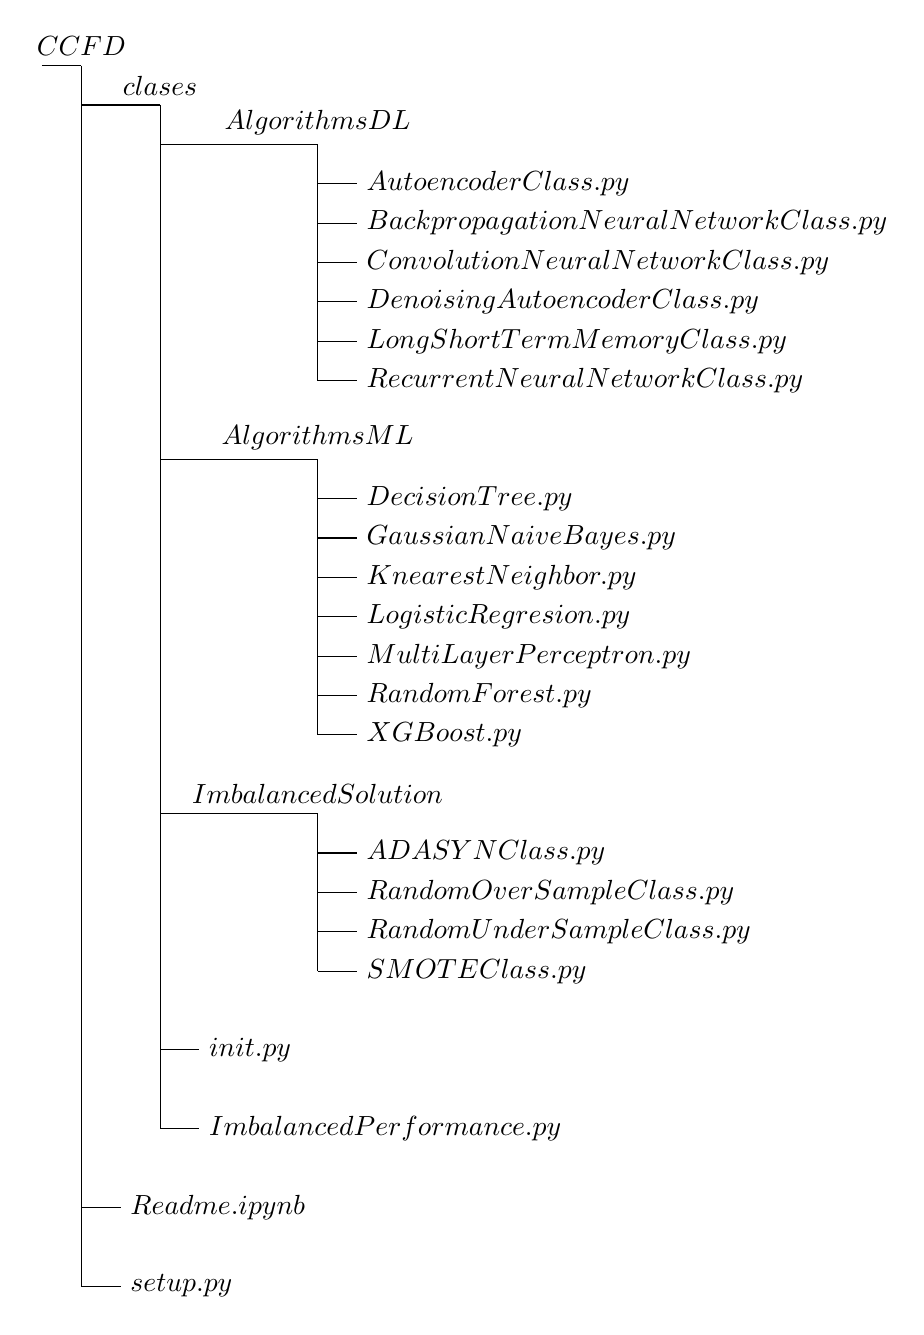
\begin{tikzpicture} % jerarqu\'{i}a de la librer\'{i}a
		% Nivel principal
		\draw (0,-0.5) -- (0.5,-0.5) node(xline1)[above]{$CCFD$};
		\draw (0.5,-0.5) -- (0.5,-1.) node(yline1)[above] {$$};
		\draw (0.5,-1) -- (0.5,-1) node(N1-1)[right] {$$};
		\draw (0.5,-1) -- (1.5,-1) node(clases)[above] {$clases$};
		\draw (0.5,-1) -- (0.5,-15) node(N1-2)[right] {$$};
		\draw (0.5,-15) -- (1,-15) node(readme)[right] {$Readme.ipynb$};
		\draw (0.5,-15) -- (0.5,-16) node(N1-3)[right] {$$};
		\draw (0.5,-16) -- (1,-16) node(setup)[right] {$setup.py$};
		% Nivel clases
		\draw (1.5,-1) -- (1.5,-1.5) node(N2-1)[right] {$$};
		\draw (1.5,-1.5) -- (3.5,-1.5) node(ADL)[above] {$AlgorithmsDL$};
		\draw (1.5,-1.5) -- (1.5, -5.5) node(N2-2)[right] {$$};
		\draw (1.5,-5.5) -- (3.5,-5.5) node(AML)[above] {$AlgorithmsML$};
		\draw (1.5,-5.5) -- (1.5, -10) node(N2-3)[right] {$$};
		\draw (1.5,-10) -- (3.5,-10) node(IS)[above] {$ImbalancedSolution$};
		\draw (1.5,-10) -- (1.5,-13) node(N2-4)[right] {$$};
		\draw (1.5,-13) -- (2,-13) node(init)[right] {$init.py$};
		\draw (1.5,-13) -- (1.5,-14) node(N2-5)[right] {$$};
		\draw (1.5,-14) -- (2,-14) node(IP)[right] {$ImbalancedPerformance.py$};
		% Nivel AlgorithmsDL
		\draw (3.5,-1.5) -- (3.5,-4.5) node(N3-1)[right] {$$};
		\draw (3.5,-2) -- (4,-2) node(AEClass)[right] {$AutoencoderClass.py$};
		\draw (3.5,-2.5) -- (4,-2.5) node(BPNNClass)[right] {$BackpropagationNeuralNetworkClass.py$};
		\draw (3.5,-3) -- (4,-3) node(CNNClass)[right] {$ConvolutionNeuralNetworkClass.py$};
		\draw (3.5,-3.5) -- (4,-3.5) node(DAEClass)[right] {$DenoisingAutoencoderClass.py$};
		\draw (3.5,-4) -- (4,-4) node(LSTMClass)[right] {$LongShortTermMemoryClass.py$};
		\draw (3.5,-4.5) -- (4,-4.5) node(RNNClass)[right] {$RecurrentNeuralNetworkClass.py$};
		% Nivel AlgorithmsML
		\draw (3.5,-5.5) -- (3.5,-9) node(N3-2)[right] {$$};
		\draw (3.5,-6) -- (4,-6) node(DT)[right] {$DecisionTree.py$};
		\draw (3.5,-6.5) -- (4,-6.5) node(GNB)[right] {$GaussianNaiveBayes.py$};
		\draw (3.5,-7) -- (4,-7) node(KNN)[right] {$KnearestNeighbor.py$};
		\draw (3.5,-7.5) -- (4,-7.5) node(LR)[right] {$LogisticRegresion.py$};
		\draw (3.5,-8) -- (4,-8) node(MLP)[right] {$MultiLayerPerceptron.py$};
		\draw (3.5,-8.5) -- (4,-8.5) node(RF)[right] {$RandomForest.py$};
		\draw (3.5,-9) -- (4,-9) node(XGB)[right] {$XGBoost.py$};
		% Nivel ImbalancedSolution
		\draw (3.5,-10) -- (3.5,-12) node(N3-3)[right] {$$};
		\draw (3.5,-10.5) -- (4,-10.5) node(ADASYN)[right] {$ADASYNClass.py$};
		\draw (3.5,-11) -- (4,-11) node(ROS)[right] {$RandomOverSampleClass.py$};
		\draw (3.5,-11.5) -- (4,-11.5) node(RUS)[right] {$RandomUnderSampleClass.py$};
		\draw (3.5,-12) -- (4,-12) node(SMOTE)[right] {$SMOTEClass.py$};
	\end{tikzpicture}
	\caption{Arquitectura de la librer\'{i}a CCFD}
	\label{ff:3}
\end{figure}

  \subsection{Componentes de las soluciones al desbalance}
    Las estrategias que se aplican en la soluci\'{o}n son las utilizadas anteriormente en los experimentos realizados. Estas estrategias est\'{a}n implementadas en la librer\'{i}a \textit{imblearn}, siendo un componente reutilizable que va a ser integrado con la librer\'{i}a \textit{sklearn} para dividir los datos en conjuntos de entrenamiento y prueba. Otro componente es \textit{pandas}, muy necesario para la lectura del conjunto de datos, en este caso de un documento \textit{Excel}. Cada componente posee una clase con las siguientes funcionalidades:
    
    \begin{align}
    	 red\_data(self,csv,test\_size=0.2)\\
    	 strategy(self)\\
    	 show\_test(self) 
    \end{align}
    
    
    La primera funcionalidad va orientada a la lectura del conjunto de datos y su divisi\'{o}n en los conjuntos de entrenamiento y prueba. Para ello recibe $csv$ como la direcci\'{o}n del archivo que almacena el conjunto de datos, y $test\_size$ como la proporci\'{o}n deseada para el conjunto de prueba con respecto al conjunto general. En la segunda funcionalidad se usa el nombre strategy como gen\'{e}rica para referirse a cada una de las estrategias dependiendo del componente. Luego de ser le\'{i}dos y particionados los datos, esta funcionalidad aplica la estrategia al conjunto de entrenamiento. Y la \'{u}ltima funcionalidad, simplemente imprime por consola los \textit{shape} de los conjuntos de entrenamiento y prueba, tanto a los que tienen aplicados la estrategia como los originales.
    
    Estos componentes permiten la obtenci\'{o}n de los conjuntos de datos de entrenamiento y prueba con estrategias aplicadas, los cuales ser\'{u}n utilizados en los modelos ML y DL.
  
  \subsection{Componentes de los modelos ML y DL}
  
    Los modelos ML seleccionados ya est\'{a}n implementados en las librer\'{i}as \textit{sklearn} y \textit{xgboost}, por lo que es un componente que ser\'{a} reutilizados. Se crea un componente por cada modelo ML utilizado en los experimentos anteriores, donde cada uno tendr\'{a} las siguientes funcionalidades:
    
    \begin{align}
    	Model(ImalancedPerformanceClass)\\
    	Modelstrategy(ImbalancedPerformanceClass)
    \end{align}
    
    Se usa Model como gen\'{e}rico para referenciar a los modelos y \textit{strategy} para referenciar a cada estrategia aplicada. \textit{ImbalancedPerformanceClass} hace referencia al componente que se explicar\'{a} despu\'{e}s, del cual extrae los conjuntos de entrenamiento y prueba de la estrategia seleccionada. En el caso de la primera funcionalidad, se devuelve una lista con un modelo por cada estrategia, siendo un total de 5, y la segunda funcionalidad, devuelve una lista con un \'{u}nico modelo dependiendo de la estrategia especificada. Cada modelo posee la siguiente estructura $(name,model,X\_train,y\_train,X\_test,y\_test)$, donde \textit{name} especifica el nombre del modelo con la estrategia, \textit{model} es el modelo, $X\_train$ y $y\_train$ es el conjunto de entrenamiento con, $y$, $X\_test$ y $y\_test$ es el conjunto de prueba.
    
    Con respecto a los modelos DL, no existe ninguna librer\'{i}a que tenga implementada las arquitecturas de los modelos seleccionados en el cap\'{i}tulo anterior. Es por ello que los componentes de cada modelo DL utiliza las mismas funcionalidades que los componentes de los modelos ML, a diferencia que en los elementos de las listas no existe \textit{model}.
  
  \subsection{Integraci\'{o}n de los componentes}
    Para la integraci\'{o}n de los componentes anteriores se desarrolla el componente \textit{ImbalancedPerformance.py}, donde mediante la clase $ImbalancedPerformanceClass$ se utilizan los componentes de soluciones al desbalance, de los modelos ML y DL, adem\'{a}s de implementar los modelos DL. Las funcionalidades que posee este componente se pueden resumir en las siguientes:
    
  \begin{align}
  	solve\_imbalanced(self,csv,test\_size=0.2)\\ 
  	performanceML(self,model)\\
  	performanceDL(self,model,dropout=[0.5,0.4,0.3])\\
  	show\_comparison(self)\\ 
  	show\_comparison\_*(self)\\
  \end{align}
  
  La primera funcionalidad se encarga de obtener todos los conjuntos de entrenamiento y prueba por cada estrategia, y almacenarlas para su pr\'{o}xima utilizaci\'{o}n. Los par\'{a}metros son los mismos que la funcionalidad $red\_data(\dots)$ de los componentes de soluciones al desbalance. La segunda funcionalidad se utiliza para realizar el entrenamiento y las pruebas, adem\'{a}s de los resultados de las m\'{e}tricas de los modelos pasados por par\'{a}metro en la variable \textit{model}, los cuales son almacenados.
  
  En la tercera funcionalidad se utiliza DL como gen\'{e}rico para referenciar a los modelos DL. A diferencia de la segunda funcionalidad, este posee el par\'{a}metro \textit{dropout}, utilizados en algunos modelos para definir el valor que tendr\'{a}n los \textit{dropouts} en esos modelos, adem\'{a}s de que se implementan los modelos. En la cuarta y quinta funcionalidad se crean \textit{Data Frames} a partir de los resultados obtenidos y almacenados de la segunda y tercera funcionalidad. El * hace referencia a variantes de la cuarta funcionalidad, donde se abarcan o difieren en algunos atributos. Esta funcionalidad devuelve dichos \textit{Data Frames}.
  
  De esta forma queda desarrollada generalmente la librer\'{i}a \textit{CCFD}, permitiendo a los usuarios realizar experimentos y pruebas a distintos conjuntos de datos.
  
	\chapter*{Conclusiones generales}

Los resultados de este trabajo han sido satisfactorios y cumplen con los objetivos propuestos para solucionar la problem\'{a}tica establecida. Estos junto a sus correspondientes respaldos investigativos, demouestran que los modelos DL poseen un gran resultado en la detecci\'{o}n de anomal\'{i}as, y a su vez, en la detecci\'{o}n de fraude en tarjetas de cr\'{e}dito. Son adem\'{a}s, la mejor opci\'{o}n cuando se trata de trabajar con \textit{Big Data}, ya que los modelos ML pierden efectividad cuando aumenta el c\'{u}mulo de datos que procesa en la detecci\'{o}, creando un sobre-entrenamiento del modelo. El sobre-entrenamiento tambi\'{e}n puede afectar a los modelos DL, pero en este caso es solucionable con el correcto ajuste de los par\'{a}metros, lo que es una de las otras grandes ventajas de estos modelos. Tambi\'{e}n son personalizables, esto se debe a que se le pueden cambiar la cantidad y el tipo de capas que se utilizan para la clasificaci\'{o}n, incluso la cantidad de neuronas que posee cada capa. Mediante la experimentaci\'{o}n se han podido obtener grandes resultados, los cuales evidencian una gran superioridad de los modelos DL con respecto a los modelos ML. A continuaci\'{o}n los principales resultados que se obtuvieron:

\begin{itemize}
	\item El modelo CNN obtiene mejores resultados con los datos desbalanceados, siendo el m\'{a}s efectivo en la detecci\'{o}n de fraude de tarjeta de cr\'{e}dito cuando existe desbalance de la informaci\'{o}n.
	\item El modelo BPNN obtiene los mejores resultados en cuanto a las estrategias aplicadas para solucionar el desbalance de la informaci\'{o}n, a pesar de obtener resultados id\'{e}nticos con los modelos AE, DAE, RNN y LSTM, este posee mayor precisi\'{o}n.
	\item En los modelos AE, DAE, RNN y LSTM, se aprecian igualdad en los resultados en cuanto a las pruebas, sin embargo su gran diferencia se puede observar en el entrenamiento de los mismos.
	\item En cuanto a la divisi\'{o}n del conjunto de datos, se aprecia que a medida que aumenta el porcentaje de datos para el entrenamiento, mejoran los resultados de \textit{F1 Score}, pero a su vez disminuye la precisi\'{o}n con que se detectan los fraudes. Es por ello es importante encontrar un procentaje donde ambas m\'{e}tricas se encuentren equilibradas.
	\item El \textit{overfitting} afecta tambi\'{e}n a los modelos DL por lo que es necesario aplicar el \textit{dropout regularization}, de esta forma se reajusta el modelo.
	\item \textit{Random Forest} result\'{o} como el mejor modelo dentro de los modelos ML, obteniendo los mejores resultados en las m\'{e}tricas de estudio.
\end{itemize}

Los resultados obtenidos en la experimentaci\'{o}n definieron las bases para el desarrollo de una librer\'{i}a Python, la cual nos permite ajustar par\'{a}metros de los modelos. Esta librer\'{i}a es un proycto en desarrollo, acutalmente solo es ajustable el orden de los \textit{dropouts} y la cantidad de \textit{epochs}. Actualmente la librer\'{i}a permite el uso de los modelos ML y DL utilizados en la experimentaci\'{o}n.

	\begin{thebibliography}{a}
	\bibitem{1} \textsc{Economipedia}. \textit{Funciones de los bancos - Definici\'{o}n, qu\'{e} es y concepto}. Accedido 20 de mayo de 2021. \url{https://economipedia.com/definiciones/funciones-de-los-bancos.html}.
	\bibitem{2} \textsc{Ilyas, Sadaf, Sultan Zia, Zaib un Nisa, Umair Muneer Butt, y Sukumar Letchmunan}. \textit{Predicting the Future Transaction from Large an Imbalanced Banking Dataset}. IJACSA, 2020.
	\bibitem{3} \textsc{Technology partner for innovative companies}. \textit{Machine Learning in Banking - Opportunities, Risks, Use Cases}, 4 de febrero de 2021. \url{https://spd.group/machine-learning/machine-learning-in-banking/}.
	\bibitem{4} \textsc{Trivedi, Naresh, Sarita Simaiya, Dr Kumar, y Sanjeev Sharma}. \textit{An Efficient Credit Card Fraud Detection Model Based on Machine Learning Methods}. MATTER: International Journal of Science and Technology, 1 de enero de 2020.
	\bibitem{5} \textsc{Lima, Servio}. \textit{Deep Learning for Fraud Detection in the Banking Industry}. Human IST Institute, diciembre de 2018.
	\bibitem{6} \textsc{Boucher, \'{E}glantine}. \textit{Outlier Detection Methods Applied to Financial Fraud}, 2020.
	\bibitem{7} \textsc{Brownlee, Jason}. \textit{A Gentle Introduction to Imbalanced Classification}. Machine Learning Mastery (blog), 22 de diciembre de 2019. \url{https://machinelearningmastery.com/what-is-imbalanced-classification/}.
	\bibitem{8} \textit{Undersampling Algorithms for Imbalanced Classification}. Accedido 5 de julio de 2021. \url{https://machinelearningmastery.com/undersampling-algorithms-for-imbalanced-classification/}.
	\bibitem{9} \textsc{Brownlee, Jason}. \textit{Random Oversampling and Undersampling for Imbalanced Classification}. Machine Learning Mastery (blog), 14 de enero de 2020. \url{https://machinelearningmastery.com/random-oversampling-and-undersampling-for-imbalanced-classification/}.
	\bibitem{10} \textsc{Brownlee, Jason}. \textit{SMOTE for Imbalanced Classification with Python}, 17 de enero de 2021. \url{https://machinelearningmastery.com/smote-oversampling-for-imbalanced-classification/.}
	\bibitem{11} \textsc{Rui Nian}. \textit{Fixing Imbalanced Datasets: An Introduction to ADASYN (with code!)}. Medium. Accedido 5 de julio de 2021. \url{https://medium.com/@ruinian/an-introduction-to-adasyn-with-code-1383a5ece7aa}.
	\bibitem{12} \textsc{Sun, Bo, y Haiyan Chen}. \textit{A survey of k Nearest Neighbor Algorithms for Solving the Class Imbalanced Problem}, 17 de enero de 2021.
	\bibitem{13} \textit{Big Data}. Investopedia. Accedido 27 de mayo de 2021. \url{https://www.investopedia.com/terms/b/big-data.asp}.
	\bibitem{14} \textsc{Thudumu, Srikanth, Philip Branch, Jiong Jin, y Jugdutt (Jack) Singh}. \textit{A Comprehensive Survey of Anomaly Detection Techniques for High Dimensional Big Data}. Journal of Big Data 7, n.o 1 (diciembre de 2020): 42. \url{https://doi.org/10.1186/s40537-020-00320-x}.
	\bibitem{15} \textsc{Huang, Jian, Junyi Chai, y Stella Cho}. \textit{Deep learning in finance and banking: A literature review and clasification}, 2020. \url{https://doi.org/10.1186/s11782-020-00082-6}.
	\bibitem{16} \textsc{Nguyen, Thanh Thi, Hammad Tahir, Mohamed Abdelrazek, y Ali Babar}. \textit{Deep Learning Methods for Credit Card Fraud Detection}, s. f., 8.
	\bibitem{17} \textsc{Mohammed V, Rabat, Morocco, Ibtissam Benchaji, Samira Douzi, y Bouabid El Ouahidi}. \textit{Credit Card Fraud Detection Model Based on LSTM Recurrent Neural Networks}. Faculty of Sciences IPSS, University, Journal of Advances in Information Technology 12, n.o 2 (2021): 113-18. \url{https://doi.org/10.12720/jait.12.2.113-118}.
	\bibitem{18} \textsc{Nengcheng, Chen, Xiong Chang, Du Wenying, Wang Chao, Lin Xin, y Chen Zeqiang}. \textit{An Improved Genetic Algorithm Couplin a Back-Propagation Neural Network Model (IGA-BPNN) for Water-Level Predictions}, 30 de junio de 2019.
	\bibitem{19} \textit{Denoising Autoencoders with Keras, TensorFlow, and Deep Learning}, PyImageSearch, 24 de febrero de 2020. \url{https://www.pyimagesearch.com/2020/02/24/denoising-autoencoders-with-keras-tensorflow-and-deep-learning/}.
	\bibitem{20} \textsc{Brownlee, Jason}. \textit{Dropout Regularization in Deep Learning Models With Keras}. Machine Learning Mastery (blog), 19 de junio de 2016. \url{https://machinelearningmastery.com/dropout-regularization-deep-learning-models-keras/}.
	\bibitem{21} \textit{Clasificaci\'{o}n con datos desbalanceados | Aprende Machine Learning}. Accedido 7 de septiembre de 2021. \url{https://www.aprendemachinelearning.com/clasificacion-con-datos-desbalanceados/}.
	\bibitem{22} \textit{Keras: the Python deep learning API}. Accedido 3 de julio de 2021. \url{https://keras.io/}.
	\bibitem{23} \textit{Introduction to NumPy}. Accedido 3 de julio de 2021. \url{https://www.w3schools.com/python/numpy/numpy_intro.asp}.
	\bibitem{24} \textit{pandas PyPI}. Accedido 3 de julio de 2021. \url{https://pypi.org/project/pandas/}.
	\bibitem{25} \textit{scikit-learn: machine learning in Python - scikit-learn 0.24.2 documentation}. Accedido 3 de julio de 2021. \url{https://scikit-learn.org/stable/}.
	\bibitem{26} \textit{Matplotlib: Python plotting - Matplotlib 3.4.2 documentation}. Accedido 3 de julio de 2021. \url{https://matplotlib.org/}.
	\bibitem{27} \textit{imbalanced-learn documentation - Version 0.8.0}. Accedido 5 de julio de 2021. \url{https://imbalanced-learn.org/stable/}.
	\bibitem{28} \textit{PyCharm: the Python IDE for Professional Developers by JetBrains}. Accedido 5 de julio de 2021. \url{https://www.jetbrains.com/pycharm/}.
	\bibitem{29} \textsc{ITELLIGENT INFORMATION TECHNOLOGIES}. \textit{10 ventajas de la miner\'{i}a de datos}, 4 de agosto de 2016. \url{https://itelligent.es/es/10-ventajas-la-mineria-web/}.
	\bibitem{30} \textit{Sesion5\_Metodologias.pdf}. Accedido 3 de julio de 2021. \url{https://disi.unal.edu.co/~eleonguz/cursos/md/presentaciones/Sesion5\_Metodologias.pdf}.
	\bibitem{31} \textsc{Maimon, Oded, y Lior Rokach}, eds. Data Mining and Knowledge Discovery Handbook. Boston, MA: Springer US, 2010. \url{https://doi.org/10.1007/978-0-387-09823-4}.
	\bibitem{32} \textit{Redes neuronales con Python}. Accedido 13 de septiembre de 2021. \url{https://www.cienciadedatos.net/documentos/py35-redes-neuronales-python.html}.
	\bibitem{33} \textsc{Bushaev, Vitaly}. \textit{Adam - Latest Trends in Deep Learning Optimization.} Medium, 24 de octubre de 2018. \url{https://towardsdatascience.com/adam-latest-trends-in-deep-learning-optimization-6be9a291375c}.
\end{thebibliography}

	\chapter*{Anexos}

\begin{figure}[h!]
	\centering
	\includegraphics[width=0.8\textwidth]{"figuras/Experimento2/ML_Imbalanced_test"}
	\caption{Puntuaciones de las pruebas de los modelos ML con datos desbalanceados.}
	\label{an:1}
\end{figure}

\begin{figure}[h!]
	\centering
	\includegraphics[width=0.8\textwidth]{"figuras/Experimento2/ML_UnderSampler_test"}
	\caption{Puntuaciones de las pruebas de los modelos ML con UnderSampler.}
	\label{an:2}
\end{figure}

\begin{figure}[h!]
	\centering
	\includegraphics[width=0.8\textwidth]{"figuras/Experimento2/ML_OverSampler_test"}
	\caption{Puntuaciones de las pruebas de los modelos ML con OverSampler.}
	\label{an:3}
\end{figure}

\begin{figure}[h!]
	\centering
	\includegraphics[width=0.8\textwidth]{"figuras/Experimento2/ML_SMOTE_test"}
	\caption{Puntuaciones de las pruebas de los modelos ML con SMOTE.}
	\label{an:4}
\end{figure}

\begin{figure}[h!]
	\centering
	\includegraphics[width=0.8\textwidth]{"figuras/Experimento2/ML_ADASYN_test"}
	\caption{Puntuaciones de las pruebas de los modelos ML con ADASYN.}
	\label{an:5}
\end{figure}

\begin{longtable}{|c|c|c|c|c|c|c|}
	\hline
	Epoch & Model & Accuracy & AUC & Precision & Recall & F1\\ \hline
	\endfirsthead
	\hline
	Epoch & Model & Accuracy & AUC & Precision & Recall & F1\\ \hline
	\endhead
	1 & CNN IMBALANCE & \colorbox{green}{0.99675} & 0.566667 & \colorbox{green}{0.996761} & \colorbox{green}{0.99675} & \colorbox{green}{0.99551}\\ \hline
	50 & CNN IMBALANCE & \colorbox{green}{0.99675} & 0.566667 & \colorbox{green}{0.996761} & \colorbox{green}{0.99675} & \colorbox{green}{0.99551}\\ \hline
	20 & CNN IMBALANCE & \colorbox{yellow}{0.9965} & 0.566541 & 0.99551 & \colorbox{yellow}{0.9965} & \colorbox{yellow}{0.995336}\\ \hline
	100 & CNN IMBALANCE & 0.99625 & 0.566416 & 0.994884 & 0.99625 & 0.995167\\ \hline
	1 & DAE IMBALANCE & 0.99625 & 0.5 & 0.992514 & 0.99625 & 0.994379\\ \hline
	50 & DAE UNDERSAMPLE & 0.99625 & 0.5 & 0.992514 & 0.99625 & 0.994379\\ \hline
	20 & AE UNDERSAMPLE & 0.99625 & 0.5 & 0.992514 & 0.99625 & 0.994379\\ \hline
	20 & DAE UNDERSAMPLE & 0.99625 & 0.5 & 0.992514 & 0.99625 & 0.994379\\ \hline
	20 & RNN UNDERSAMPLE & 0.99625 & 0.5 & 0.992514 & 0.99625 & 0.994379\\ \hline
	20 & LSTM UNDERSAMPLE & 0.99625 & 0.5 & 0.992514 & 0.99625 & 0.994379\\ \hline
	20 & BPNN UNDERSAMPLE & 0.99625 & 0.5 & 0.996264 & 0.99625 & 0.994379\\ \hline
	1 & AE IMBALANCE & 0.99625 & 0.5 & 0.992514 & 0.99625 & 0.994379\\ \hline
	1 & RNN IMBALANCE & 0.99625 & 0.5 & 0.992514 & 0.99625 & 0.994379\\ \hline
	50 & DAE IMBALANCE & 0.99625 & 0.5 & 0.992514 & 0.99625 & 0.994379\\ \hline
	50 & RNN IMBALANCE & 0.99625 & 0.5 & 0.992514 & 0.99625 & 0.994379\\ \hline
	50 & LSTM IMBALANCE & 0.99625 & 0.5 & 0.992514 & 0.99625 & 0.994379\\ \hline
	50 & BPNN IMBALANCE & 0.99625 & 0.5 & 0.996264 & 0.99625 & 0.994379\\ \hline
	50 & AE UNDERSAMPLE & 0.99625 & 0.5 & 0.992514 & 0.99625 & 0.994379\\ \hline
	50 & RNN UNDERSAMPLE & 0.99625 & 0.5 & 0.992514 & 0.99625 & 0.994379\\ \hline
	20 & LSTM IMBALANCE & 0.99625 & 0.5 & 0.992514 & 0.99625 & 0.994379\\ \hline
	50 & LSTM UNDERSAMPLE & 0.99625 & 0.5 & 0.992514 & 0.99625 & 0.994379\\ \hline
	50 & BPNN UNDERSAMPLE & 0.99625 & 0.5 & 0.996264 & 0.99625 & 0.994379\\ \hline
	100 & AE IMBALANCE & 0.99625 & 0.5 & 0.992514 & 0.99625 & 0.994379\\ \hline
	100 & DAE IMBALANCE & 0.99625 & 0.5 & 0.992514 & 0.99625 & 0.994379\\ \hline
	100 & RNN IMBALANCE & 0.99625 & 0.5 & 0.992514 & 0.99625 & 0.994379\\ \hline
	100 & LSTM IMBALANCE & 0.99625 & 0.5 & 0.992514 & 0.99625 & 0.994379\\ \hline
	100 & BPNN IMBALANCE & 0.99625 & 0.5 & 0.996264 & 0.99625 & 0.994379\\ \hline
	100 & AE UNDERSAMPLE & 0.99625 & 0.5 & 0.992514 & 0.99625 & 0.994379\\ \hline
	100 & DAE UNDERSAMPLE & 0.99625 & 0.5 & 0.992514 & 0.99625 & 0.994379\\ \hline
	100 & RNN UNDERSAMPLE & 0.99625 & 0.5 & 0.992514 & 0.99625 & 0.994379\\ \hline
	100 & LSTM UNDERSAMPLE & 0.99625 & 0.5 & 0.992514 & 0.99625 & 0.994379\\ \hline
	100 & BPNN UNDERSAMPLE & 0.99625 & 0.5 & 0.996264 & 0.99625 & 0.994379\\ \hline
	20 & BPNN IMBALANCE & 0.99625 & 0.5 & 0.996264 & 0.99625 & 0.994379\\ \hline
	50 & AE IMBALANCE & 0.99625 & 0.5 & 0.992514 & 0.99625 & 0.994379\\ \hline
	20 & RNN IMBALANCE & 0.99625 & 0.5 & 0.992514 & 0.99625 & 0.994379\\ \hline
	1 & LSTM IMBALANCE & 0.99625 & 0.5 & 0.992514 & 0.99625 & 0.994379\\ \hline
	20 & DAE IMBALANCE & 0.99625 & 0.5 & 0.992514 & 0.99625 & 0.994379\\ \hline
	1 & BPNN UNDERSAMPLE & 0.99625 & 0.5 & 0.996264 & 0.99625 & 0.994379\\ \hline
	1 & LSTM UNDERSAMPLE & 0.99625 & 0.5 & 0.992514 & 0.99625 & 0.994379\\ \hline
	1 & DAE UNDERSAMPLE & 0.99625 & 0.5 & 0.992514 & 0.99625 & 0.994379\\ \hline
	1 & AE UNDERSAMPLE & 0.99625 & 0.5 & 0.992514 & 0.99625 & 0.994379\\ \hline
	1 & BPNN IMBALANCE & 0.99625 & 0.5 & 0.996264 & 0.99625 & 0.994379\\ \hline
	1 & RNN UNDERSAMPLE & 0.99625 & 0.5 & 0.992514 & 0.99625 & 0.994379\\ \hline
	20 & AE IMBALANCE & 0.99625 & 0.5 & 0.992514 & 0.99625 & 0.994379\\ \hline
	100 & AE OVERSAMPLE & 0.99575 & 0.5 & 0.991518 & 0.99575 & 0.99363\\ \hline
	100 & DAE OVERSAMPLE & 0.99575 & 0.5 & 0.991518 & 0.99575 & 0.99363\\ \hline
	100 & RNN OVERSAMPLE & 0.99575 & 0.5 & 0.991518 & 0.99575 & 0.99363\\ \hline
	1 & BPNN OVERSAMPLE & 0.99575 & 0.5 & 0.995768 & 0.99575 & 0.99363\\ \hline
	100 & LSTM OVERSAMPLE & 0.99575 & 0.5 & 0.991518 & 0.99575 & 0.99363\\ \hline
	1 & AE OVERSAMPLE & 0.99575 & 0.5 & 0.991518 & 0.99575 & 0.99363\\ \hline
	1 & DAE OVERSAMPLE & 0.99575 & 0.5 & 0.991518 & 0.99575 & 0.99363\\ \hline
	100 & BPNN OVERSAMPLE & 0.99575 & 0.5 & 0.995768 & 0.99575 & 0.99363\\ \hline
	50 & LSTM OVERSAMPLE & 0.99575 & 0.5 & 0.991518 & 0.99575 & 0.99363\\ \hline
	50 & RNN OVERSAMPLE & 0.99575 & 0.5 & 0.991518 & 0.99575 & 0.99363\\ \hline
	50 & DAE OVERSAMPLE & 0.99575 & 0.5 & 0.991518 & 0.99575 & 0.99363\\ \hline
	50 & AE OVERSAMPLE & 0.99575 & 0.5 & 0.991518 & 0.99575 & 0.99363\\ \hline
	1 & RNN OVERSAMPLE & 0.99575 & 0.5 & 0.995768 & 0.99575 & 0.99363\\ \hline
	1 & LSTM OVERSAMPLE & 0.99575 & 0.5 & 0.991518 & 0.99575 & 0.99363\\ \hline
	50 & BPNN OVERSAMPLE & 0.99575 & 0.5 & 0.995768 & 0.99575 & 0.99363\\ \hline
	20 & LSTM OVERSAMPLE & 0.99575 & 0.5 & 0.991518 & 0.99575 & 0.99363\\ \hline
	20 & RNN OVERSAMPLE & 0.99575 & 0.5 & 0.991518 & 0.99575 & 0.99363\\ \hline
	20 & DAE OVERSAMPLE & 0.99575 & 0.5 & 0.991518 & 0.99575 & 0.99363\\ \hline
	20 & AE OVERSAMPLE & 0.99575 & 0.5 & 0.991518 & 0.99575 & 0.99363\\ \hline
	20 & BPNN OVERSAMPLE & 0.99575 & 0.5 & 0.995768 & 0.99575 & 0.99363\\ \hline
	100 & AE SMOTE & 0.9955 & 0.5 & 0.99102 & 0.9955 & 0.993255\\ \hline
	20 & AE SMOTE & 0.9955 & 0.5 & 0.99102 & 0.9955 & 0.993255\\ \hline
	20 & DAE SMOTE & 0.9955 & 0.5 & 0.99102 & 0.9955 & 0.993255\\ \hline
	50 & BPNN SMOTE & 0.9955 & 0.5 & 0.99552 & 0.9955 & 0.993255\\ \hline
	50 & LSTM SMOTE & 0.9955 & 0.5 & 0.99102 & 0.9955 & 0.993255\\ \hline
	50 & RNN SMOTE & 0.9955 & 0.5 & 0.99102 & 0.9955 & 0.993255\\ \hline
	50 & DAE SMOTE & 0.9955 & 0.5 & 0.99102 & 0.9955 & 0.993255\\ \hline
	50 & AE SMOTE & 0.9955 & 0.5 & 0.99102 & 0.9955 & 0.993255\\ \hline
	20 & RNN SMOTE & 0.9955 & 0.5 & 0.99102 & 0.9955 & 0.993255\\ \hline
	20 & BPNN SMOTE & 0.9955 & 0.5 & 0.99552 & 0.9955 & 0.993255\\ \hline
	20 & LSTM SMOTE & 0.9955 & 0.5 & 0.99102 & 0.9955 & 0.993255\\ \hline
	100 & DAE SMOTE & 0.9955 & 0.5 & 0.99102 & 0.9955 & 0.993255\\ \hline
	100 & LSTM SMOTE & 0.9955 & 0.5 & 0.99102 & 0.9955 & 0.993255\\ \hline
	100 & BPNN SMOTE & 0.9955 & 0.5 & 0.99552 & 0.9955 & 0.993255\\ \hline
	1 & BPNN SMOTE & 0.9955 & 0.5 & 0.99552 & 0.9955 & 0.993255\\ \hline
	1 & LSTM SMOTE & 0.9955 & 0.5 & 0.99102 & 0.9955 & 0.993255\\ \hline
	1 & AE SMOTE & 0.9955 & 0.5 & 0.99102 & 0.9955 & 0.993255\\ \hline
	1 & RNN SMOTE & 0.9955 & 0.5 & 0.99102 & 0.9955 & 0.993255\\ \hline
	100 & RNN SMOTE & 0.9955 & 0.5 & 0.99102 & 0.9955 & 0.993255\\ \hline
	1 & DAE SMOTE & 0.9955 & 0.5 & 0.99102 & 0.9955 & 0.993255\\ \hline
	1 & DAE ADASYN & 0.99525 & 0.5 & \colorbox{red}{0.990523} & 0.99525 & 0.992881\\ \hline
	100 & LSTM ADASYN & 0.99525 & 0.5 & \colorbox{red}{0.990523} & 0.99525 & 0.992881\\ \hline
	1 & LSTM ADASYN & 0.99525 & 0.5 & \colorbox{red}{0.990523} & 0.99525 & 0.992881\\ \hline
	1 & RNN ADASYN & 0.99525 & 0.5 & \colorbox{red}{0.990523} & 0.99525 & 0.992881\\ \hline
	100 & RNN ADASYN & 0.99525 & 0.5 & \colorbox{red}{0.990523} & 0.99525 & 0.992881\\ \hline
	100 & DAE ADASYN & 0.99525 & 0.5 & \colorbox{red}{0.990523} & 0.99525 & 0.992881\\ \hline
	100 & AE ADASYN & 0.99525 & 0.5 & \colorbox{red}{0.990523} & 0.99525 & 0.992881\\ \hline
	1 & BPNN ADASYN & 0.99525 & 0.5 & 0.995273 & 0.99525 & 0.992881\\ \hline
	20 & BPNN ADASYN & 0.99525 & 0.5 & 0.995273 & 0.99525 & 0.992881\\ \hline
	50 & BPNN ADASYN & 0.99525 & 0.5 & 0.995273 & 0.99525 & 0.992881\\ \hline
	100 & BPNN ADASYN & 0.99525 & 0.5 & 0.995273 & 0.99525 & 0.992881\\ \hline
	20 & LSTM ADASYN & 0.99525 & 0.5 & \colorbox{red}{0.990523} & 0.99525 & 0.992881\\ \hline
	1 & AE ADASYN & 0.99525 & 0.5 & \colorbox{red}{0.990523} & 0.99525 & 0.992881\\ \hline
	50 & LSTM ADASYN & 0.99525 & 0.5 & \colorbox{red}{0.990523} & 0.99525 & 0.992881\\ \hline
	50 & RNN ADASYN & 0.99525 & 0.5 & \colorbox{red}{0.990523} & 0.99525 & 0.992881\\ \hline
	20 & RNN ADASYN & 0.99525 & 0.5 & \colorbox{red}{0.990523} & 0.99525 & 0.992881\\ \hline
	20 & DAE ADASYN & 0.99525 & 0.5 & \colorbox{red}{0.990523} & 0.99525 & 0.992881\\ \hline
	50 & DAE ADASYN & 0.99525 & 0.5 & \colorbox{red}{0.990523} & 0.99525 & 0.992881\\ \hline
	50 & AE ADASYN & 0.99525 & 0.5 & \colorbox{red}{0.990523} & 0.99525 & 0.992881\\ \hline
	20 & AE ADASYN & 0.99525 & 0.5 & \colorbox{red}{0.990523} & 0.99525 & 0.992881\\ \hline
	50 & CNN SMOTE & 0.99225 & 0.608977 & 0.992855 & 0.99225 & 0.992547\\ \hline
	100 & CNN SMOTE & 0.99125 & 0.608474 & 0.992714 & 0.99125 & 0.991958\\ \hline
	100 & CNN ADASYN & 0.99125 & 0.628941 & 0.992657 & 0.99125 & 0.991927\\ \hline
	50 & CNN ADASYN & \colorbox{red}{0.99} & 0.628313 & 0.992506 & 0.99 & 0.991192\\ \hline
	20 & CNN SMOTE & 0.98975 & 0.607721 & 0.992569 & 0.98975 & 0.991101\\ \hline
	100 & CNN OVERSAMPLE & 0.9875 & \colorbox{yellow}{0.700861} & 0.993864 & 0.9875 & 0.990406\\ \hline
	50 & CNN OVERSAMPLE & 0.9865 & 0.700359 & 0.993812 & 0.9865 & 0.989846\\ \hline
	20 & CNN OVERSAMPLE & 0.98475 & 0.69948 & 0.993737 & 0.98475 & 0.988879\\ \hline
	20 & CNN ADASYN & 0.97925 & 0.622913 & 0.992022 & 0.97925 & 0.985314\\ \hline
	1 & CNN OVERSAMPLE & 0.93125 & \colorbox{yellow}{0.701902} & 0.993469 & 0.93125 & 0.960463\\ \hline
	100 & CNN UNDERSAMPLE & 0.76675 & 0.617273 & 0.99368 & 0.76675 & 0.864517\\ \hline
	50 & CNN UNDERSAMPLE & 0.53675 & 0.535048 & 0.993017 & 0.53675 & 0.695181\\ \hline
	1 & CNN SMOTE & 0.39575 & 0.558248 & 0.992364 & 0.39575 & 0.562558\\ \hline
	1 & CNN ADASYN & 0.38025 & 0.531505 & 0.991331 & 0.38025 & 0.546305\\ \hline
	20 & CNN UNDERSAMPLE & \colorbox{red}{0.121} & 0.459222 & 0.989971 & 0.121 & 0.210891\\ \hline
	1 & CNN UNDERSAMPLE & 0.0765 & 0.536512 & \colorbox{yellow}{0.996265} & \colorbox{red}{0.0765} & \colorbox{red}{0.135628}\\ \hline
	\caption{Puntuaciones en las pruebas de los modelos DL por estrategias y epochs.}
	\label{an:6}
\end{longtable}

\begin{figure}[h!]
	\centering
	\includegraphics[width=0.8\textwidth]{"figuras/Experimento5/Imbalanced/DL_imbalanced_1_train"}
	\caption{Puntuaciones del entrenamiento de los modelos DL con datos desbalanceados en 1 epoch.}
	\label{an:7}
\end{figure}

\begin{figure}[h!]
	\centering
	\includegraphics[width=0.8\textwidth]{"figuras/Experimento5/Imbalanced/DL_imbalanced_20_train"}
	\caption{Puntuaciones del entrenamiento de los modelos DL con datos desbalanceados en 20 epochs.}
	\label{an:8}
\end{figure}

\begin{figure}[h!]
	\centering
	\includegraphics[width=0.8\textwidth]{"figuras/Experimento5/Imbalanced/DL_imbalanced_50_train"}
	\caption{Puntuaciones del entrenamiento de los modelos DL con datos desbalanceados en 50 epochs.}
	\label{an:9}
\end{figure}

\begin{figure}[h!]
	\centering
	\includegraphics[width=0.8\textwidth]{"figuras/Experimento5/Imbalanced/DL_imbalanced_100_train"}
	\caption{Puntuaciones del entrenamiento de los modelos DL con datos desbalanceados en 100 epochs.}
	\label{an:10}
\end{figure}

\begin{figure}[h!]
	\centering
	\includegraphics[width=0.8\textwidth]{"figuras/Experimento5/UnderSampler/DL_UnderSampler_1_train"}
	\caption{Puntuaciones del entrenamiento de los modelos DL con datos desbalanceados en 1 epoch.}
	\label{an:11}
\end{figure}

\begin{figure}[h!]
	\centering
	\includegraphics[width=0.8\textwidth]{"figuras/Experimento5/UnderSampler/DL_UnderSampler_20_train"}
	\caption{Puntuaciones del entrenamiento de los modelos DL con datos desbalanceados en 20 epochs.}
	\label{an:12}
\end{figure}

\begin{figure}[h!]
	\centering
	\includegraphics[width=0.8\textwidth]{"figuras/Experimento5/UnderSampler/DL_UnderSampler_50_train"}
	\caption{Puntuaciones del entrenamiento de los modelos DL con datos desbalanceados en 50 epochs.}
	\label{an:13}
\end{figure}

\begin{figure}[h!]
	\centering
	\includegraphics[width=0.8\textwidth]{"figuras/Experimento5/UnderSampler/DL_UnderSampler_100_train"}
	\caption{Puntuaciones del entrenamiento de los modelos DL con datos desbalanceados en 100 epochs.}
	\label{an:14}
\end{figure}

\begin{figure}[h!]
	\centering
	\includegraphics[width=0.8\textwidth]{"figuras/Experimento5/OverSampler/DL_OverSampler_1_train"}
	\caption{Puntuaciones del entrenamiento de los modelos DL con datos desbalanceados en 1 epoch.}
	\label{an:15}
\end{figure}

\begin{figure}[h!]
	\centering
	\includegraphics[width=0.8\textwidth]{"figuras/Experimento5/OverSampler/DL_OverSampler_20_train"}
	\caption{Puntuaciones del entrenamiento de los modelos DL con datos desbalanceados en 20 epochs.}
	\label{an:16}
\end{figure}

\begin{figure}[h!]
	\centering
	\includegraphics[width=0.8\textwidth]{"figuras/Experimento5/OverSampler/DL_OverSampler_50_train"}
	\caption{Puntuaciones del entrenamiento de los modelos DL con datos desbalanceados en 50 epochs.}
	\label{an:17}
\end{figure}

\begin{figure}[h!]
	\centering
	\includegraphics[width=0.8\textwidth]{"figuras/Experimento5/OverSampler/DL_OverSampler_100_train"}
	\caption{Puntuaciones del entrenamiento de los modelos DL con datos desbalanceados en 100 epochs.}
	\label{an:18}
\end{figure}

\begin{figure}[h!]
	\centering
	\includegraphics[width=0.8\textwidth]{"figuras/Experimento5/SMOTE/DL_SMOTE_1_train"}
	\caption{Puntuaciones del entrenamiento de los modelos DL con datos desbalanceados en 1 epoch.}
	\label{an:19}
\end{figure}

\begin{figure}[h!]
	\centering
	\includegraphics[width=0.8\textwidth]{"figuras/Experimento5/SMOTE/DL_SMOTE_20_train"}
	\caption{Puntuaciones del entrenamiento de los modelos DL con datos desbalanceados en 20 epochs.}
	\label{an:20}
\end{figure}

\begin{figure}[h!]
	\centering
	\includegraphics[width=0.8\textwidth]{"figuras/Experimento5/SMOTE/DL_SMOTE_50_train"}
	\caption{Puntuaciones del entrenamiento de los modelos DL con datos desbalanceados en 50 epochs.}
	\label{an:21}
\end{figure}

\begin{figure}[h!]
	\centering
	\includegraphics[width=0.8\textwidth]{"figuras/Experimento5/SMOTE/DL_SMOTE_100_train"}
	\caption{Puntuaciones del entrenamiento de los modelos DL con datos desbalanceados en 100 epochs.}
	\label{an:22}
\end{figure}

\begin{figure}[h!]
	\centering
	\includegraphics[width=0.8\textwidth]{"figuras/Experimento5/ADASYN/DL_ADASYN_1_train"}
	\caption{Puntuaciones del entrenamiento de los modelos DL con datos desbalanceados en 1 epoch.}
	\label{an:23}
\end{figure}

\begin{figure}[h!]
	\centering
	\includegraphics[width=0.8\textwidth]{"figuras/Experimento5/ADASYN/DL_ADASYN_20_train"}
	\caption{Puntuaciones del entrenamiento de los modelos DL con datos desbalanceados en 20 epochs.}
	\label{an:24}
\end{figure}

\begin{figure}[h!]
	\centering
	\includegraphics[width=0.8\textwidth]{"figuras/Experimento5/ADASYN/DL_ADASYN_50_train"}
	\caption{Puntuaciones del entrenamiento de los modelos DL con datos desbalanceados en 50 epochs.}
	\label{an:25}
\end{figure}

\begin{figure}[h!]
	\centering
	\includegraphics[width=0.8\textwidth]{"figuras/Experimento5/ADASYN/DL_ADASYN_100_train"}
	\caption{Puntuaciones del entrenamiento de los modelos DL con datos desbalanceados en 100 epochs.}
	\label{an:26}
\end{figure}

\begin{figure}[h!]
	\centering
	\includegraphics[width=0.8\textwidth]{"figuras/Experimento5/CNN/CNN_1_train"}
	\caption{Puntuaciones del entrenamiento del modelo CNN por estrategias en 1 epoch.}
	\label{an:27}
\end{figure}

\begin{figure}[h!]
	\centering
	\includegraphics[width=0.8\textwidth]{"figuras/Experimento5/CNN/CNN_20_train"}
	\caption{Puntuaciones del entrenamiento del modelo CNN por estrategias en 20 epochs.}
	\label{an:28}
\end{figure}

\begin{figure}[h!]
	\centering
	\includegraphics[width=0.8\textwidth]{"figuras/Experimento5/CNN/CNN_50_train"}
	\caption{Puntuaciones del entrenamiento del modelo CNN por estrategias en 50 epochs.}
	\label{an:29}
\end{figure}

\begin{figure}[h!]
	\centering
	\includegraphics[width=0.8\textwidth]{"figuras/Experimento5/CNN/CNN_100_train"}
	\caption{Puntuaciones del entrenamiento del modelo CNN por estrategias en 100 epochs.}
	\label{an:30}
\end{figure}

\begin{figure}[h!]
	\centering
	\includegraphics[width=0.8\textwidth]{"figuras/Experimento5/AE/AE_1_train"}
	\caption{Puntuaciones del entrenamiento del modelo AE por estrategias en 1 epoch.}
	\label{an:31}
\end{figure}

\begin{figure}[h!]
	\centering
	\includegraphics[width=0.8\textwidth]{"figuras/Experimento5/AE/AE_20_train"}
	\caption{Puntuaciones del entrenamiento del modelo AE por estrategias en 20 epochs.}
	\label{an:32}
\end{figure}

\begin{figure}[h!]
	\centering
	\includegraphics[width=0.8\textwidth]{"figuras/Experimento5/AE/AE_50_train"}
	\caption{Puntuaciones del entrenamiento del modelo AE por estrategias en 50 epochs.}
	\label{an:33}
\end{figure}

\begin{figure}[h!]
	\centering
	\includegraphics[width=0.8\textwidth]{"figuras/Experimento5/AE/AE_100_train"}
	\caption{Puntuaciones del entrenamiento del modelo AE por estrategias en 100 epochs.}
	\label{an:34}
\end{figure}

\begin{figure}[h!]
	\centering
	\includegraphics[width=0.8\textwidth]{"figuras/Experimento5/DAE/DAE_1_train"}
	\caption{Puntuaciones del entrenamiento del modelo DAE por estrategias en 1 epoch.}
	\label{an:35}
\end{figure}

\begin{figure}[h!]
	\centering
	\includegraphics[width=0.8\textwidth]{"figuras/Experimento5/DAE/DAE_20_train"}
	\caption{Puntuaciones del entrenamiento del modelo DAE por estrategias en 20 epochs.}
	\label{an:36}
\end{figure}

\begin{figure}[h!]
	\centering
	\includegraphics[width=0.8\textwidth]{"figuras/Experimento5/DAE/DAE_50_train"}
	\caption{Puntuaciones del entrenamiento del modelo DAE por estrategias en 50 epochs.}
	\label{an:37}
\end{figure}

\begin{figure}[h!]
	\centering
	\includegraphics[width=0.8\textwidth]{"figuras/Experimento5/DAE/DAE_100_train"}
	\caption{Puntuaciones del entrenamiento del modelo DAE por estrategias en 100 epochs.}
	\label{an:38}
\end{figure}

\begin{figure}[h!]
	\centering
	\includegraphics[width=0.8\textwidth]{"figuras/Experimento5/RNN/RNN_1_train"}
	\caption{Puntuaciones del entrenamiento del modelo RNN por estrategias en 1 epoch.}
	\label{an:39}
\end{figure}

\begin{figure}[h!]
	\centering
	\includegraphics[width=0.8\textwidth]{"figuras/Experimento5/RNN/RNN_20_train"}
	\caption{Puntuaciones del entrenamiento del modelo RNN por estrategias en 20 epochs.}
	\label{an:40}
\end{figure}

\begin{figure}[h!]
	\centering
	\includegraphics[width=0.8\textwidth]{"figuras/Experimento5/RNN/RNN_50_train"}
	\caption{Puntuaciones del entrenamiento del modelo RNN por estrategias en 50 epochs.}
	\label{an:41}
\end{figure}

\begin{figure}[h!]
	\centering
	\includegraphics[width=0.8\textwidth]{"figuras/Experimento5/RNN/RNN_100_train"}
	\caption{Puntuaciones del entrenamiento del modelo RNN por estrategias en 100 epochs.}
	\label{an:42}
\end{figure}

\begin{figure}[h!]
	\centering
	\includegraphics[width=0.8\textwidth]{"figuras/Experimento5/LSTM/LSTM_1_train"}
	\caption{Puntuaciones del entrenamiento del modelo LSTM por estrategias en 1 epoch.}
	\label{an:43}
\end{figure}

\begin{figure}[h!]
	\centering
	\includegraphics[width=0.8\textwidth]{"figuras/Experimento5/LSTM/LSTM_20_train"}
	\caption{Puntuaciones del entrenamiento del modelo LSTM por estrategias en 20 epochs.}
	\label{an:44}
\end{figure}

\begin{figure}[h!]
	\centering
	\includegraphics[width=0.8\textwidth]{"figuras/Experimento5/LSTM/LSTM_50_train"}
	\caption{Puntuaciones del entrenamiento del modelo LSTM por estrategias en 50 epochs.}
	\label{an:45}
\end{figure}

\begin{figure}[h!]
	\centering
	\includegraphics[width=0.8\textwidth]{"figuras/Experimento5/LSTM/LSTM_100_train"}
	\caption{Puntuaciones del entrenamiento del modelo LSTM por estrategias en 100 epochs.}
	\label{an:46}
\end{figure}

\begin{figure}[h!]
	\centering
	\includegraphics[width=0.8\textwidth]{"figuras/Experimento5/BPNN/BPNN_1_train"}
	\caption{Puntuaciones del entrenamiento del modelo BPNN por estrategias en 1 epoch.}
	\label{an:47}
\end{figure}

\begin{figure}[h!]
	\centering
	\includegraphics[width=0.8\textwidth]{"figuras/Experimento5/BPNN/BPNN_20_train"}
	\caption{Puntuaciones del entrenamiento del modelo BPNN por estrategias en 20 epochs.}
	\label{an:48}
\end{figure}

\begin{figure}[h!]
	\centering
	\includegraphics[width=0.8\textwidth]{"figuras/Experimento5/BPNN/BPNN_50_train"}
	\caption{Puntuaciones del entrenamiento del modelo BPNN por estrategias en 50 epochs.}
	\label{an:49}
\end{figure}

\begin{figure}[h!]
	\centering
	\includegraphics[width=0.8\textwidth]{"figuras/Experimento5/BPNN/BPNN_100_train"}
	\caption{Puntuaciones del entrenamiento del modelo BPNN por estrategias en 100 epochs.}
	\label{an:50}
\end{figure}

\begin{longtable}{|c|c|c|c|c|c|}
	\hline
	Epoch & Model & Accuracy Train & Precision Train & Recall Train & F1 Train\\ \hline
	\endfirsthead
	\hline
	Epoch & Model & Accuracy Train & Precision Train & Recall Train & F1 Train\\ \hline
	\endhead
	20 & CNN IMBALANCE & 0.997437477 & 0.083916076 & 0.08041957 & 0.08158508\\ \hline
	50 & CNN IMBALANCE & 0.998374999 & 0.181818172 & 0.16783215 & 0.17249417\\ \hline
	1 & CNN IMBALANCE & 0.971125007 & 0.037425533 & 0.05244755 & 0.03988132\\ \hline
	100 & CNN IMBALANCE & \colorbox{yellow}{0.998562515} & 0.181818172 & 0.18181817 & 0.17948715\\ \hline
	50 & BPNN SMOTE & 0.998307228 & \colorbox{yellow}{0.998056114} & 0.99864942 & \colorbox{yellow}{0.99829829}\\ \hline
	100 & BPNN SMOTE & 0.997523487 & 0.996707678 & 0.99837095 & 0.99745846\\ \hline
	20 & BPNN SMOTE & 0.996896565 & 0.995942354 & 0.99777555 & 0.99675047\\ \hline
	100 & BPNN UNDERSAMPLE & 0.949999988 & 0.986111104 & 0.93910253 & 0.96012986\\ \hline
	1 & BPNN SMOTE & 0.855799377 & 0.867141366 & 0.79329419 & 0.81046265\\ \hline
	50 & BPNN UNDERSAMPLE & 0.800000012 & 0.706439376 & 0.50834119 & 0.58997691\\ \hline
	20 & BPNN UNDERSAMPLE & 0.689999998 & 0.928571463 & 0.41259468 & 0.55927348\\ \hline
	50 & BPNN IMBALANCE & 0.998437524 & 0.051999997 & 0.052 & 0.052\\ \hline
	100 & BPNN IMBALANCE & 0.998437524 & 0.049999997 & 0.04899999 & 0.04933333\\ \hline
	20 & BPNN IMBALANCE & 0.99781251 & 0.033999994 & 0.03183333 & 0.0324\\ \hline
	1 & BPNN IMBALANCE & 0.940437496 & \colorbox{red}{0} & \colorbox{red}{0} & \colorbox{red}{0}\\ \hline
	1 & BPNN UNDERSAMPLE & 0.5 & \colorbox{red}{0} & \colorbox{red}{0} & \colorbox{red}{0}\\ \hline
	100 & LSTM SMOTE & 0.994576812 & 0.993465602 & 0.99562114 & 0.99436241\\ \hline
	50 & LSTM SMOTE & 0.990501583 & 0.987064838 & 0.99409676 & 0.9902218\\ \hline
	100 & RNN SMOTE & 0.984608173 & 0.981494069 & 0.98768878 & 0.9840225\\ \hline
	50 & RNN SMOTE & 0.97865206 & 0.974082828 & 0.98366153 & 0.97813684\\ \hline
	20 & RNN SMOTE & 0.97667712 & 0.971696854 & 0.98222548 & 0.97604197\\ \hline
	20 & LSTM SMOTE & 0.974043906 & 0.965691805 & 0.98348832 & 0.97362816\\ \hline
	100 & RNN UNDERSAMPLE & 0.769999981 & 0.845588207 & 0.7712912 & 0.80352724\\ \hline
	100 & LSTM UNDERSAMPLE & 0.680000007 & 0.829166651 & 0.64908314 & 0.71301317\\ \hline
	20 & DAE UNDERSAMPLE & 0.5 & 0.5546875 & \colorbox{green}{1} & 0.70659566\\ \hline
	100 & DAE UNDERSAMPLE & 0.5 & 0.5546875 & \colorbox{green}{1} & 0.70659566\\ \hline
	1 & RNN SMOTE & 0.705736697 & 0.707795322 & 0.70846796 & 0.70029038\\ \hline
	20 & LSTM UNDERSAMPLE & 0.660000026 & 0.683493614 & 0.69580197 & 0.6749922\\ \hline
	20 & RNN UNDERSAMPLE & 0.589999974 & 0.622781396 & 0.68014705 & 0.64144778\\ \hline
	50 & LSTM UNDERSAMPLE & 0.660000026 & 0.64967531 & 0.67938793 & 0.63414246\\ \hline
	50 & RNN UNDERSAMPLE & 0.589999974 & 0.576943278 & 0.55650157 & 0.56057417\\ \hline
	1 & RNN UNDERSAMPLE & 0.540000021 & 0.646139681 & 0.50062847 & 0.54794741\\ \hline
	50 & AE SMOTE & 0.497680247 & 0.401092619 & 0.80377835 & 0.53134143\\ \hline
	1 & LSTM SMOTE & 0.611347973 & 0.680008471 & 0.46954575 & 0.52970928\\ \hline
	1 & LSTM UNDERSAMPLE & 0.49000001 & 0.453070164 & 0.52777779 & 0.48501226\\ \hline
	1 & DAE SMOTE & 0.498307198 & 0.318110585 & 0.63791376 & 0.42133522\\ \hline
	1 & AE UNDERSAMPLE & 0.460000008 & 0.2890625 & 0.5 & 0.35873014\\ \hline
	100 & AE SMOTE & 0.500658333 & 0.290432364 & 0.46473235 & 0.34405035\\ \hline
	50 & DAE UNDERSAMPLE & 0.439999998 & 0.2265625 & 0.5 & 0.31111109\\ \hline
	1 & AE SMOTE & 0.495485902 & 0.245143235 & 0.45525572 & 0.30565432\\ \hline
	20 & DAE SMOTE & 0.498463959 & 0.198380858 & 0.39819458 & 0.26273957\\ \hline
	1 & DAE UNDERSAMPLE & 0.419999987 & 0.1640625 & 0.49999997 & 0.24444443\\ \hline
	20 & AE SMOTE & 0.494451404 & 0.153185934 & 0.31193581 & 0.20388429\\ \hline
	100 & DAE SMOTE & 0.498369902 & 0.13457337 & 0.27081245 & 0.17848259\\ \hline
	50 & DAE SMOTE & 0.500376165 & 0.111038476 & 0.22166499 & 0.14697345\\ \hline
	100 & LSTM IMBALANCE & 0.997687519 & 0.027999999 & 0.026 & 0.02666667\\ \hline
	50 & LSTM IMBALANCE & 0.997500002 & 0.021999998 & 0.022 & 0.022\\ \hline
	50 & RNN IMBALANCE & 0.997562528 & 0.021999998 & 0.021 & 0.02133333\\ \hline
	100 & RNN IMBALANCE & 0.997250021 & 0.017999997 & 0.017 & 0.01733333\\ \hline
	20 & LSTM IMBALANCE & 0.997187495 & 0.015999999 & 0.016 & 0.016\\ \hline
	20 & RNN IMBALANCE & 0.997250021 & 0.011999999 & 0.011 & 0.01133333\\ \hline
	1 & RNN IMBALANCE & 0.966437519 & 0.000417647 & 0.006 & 0.00077991\\ \hline
	1 & LSTM IMBALANCE & 0.99356252 & 0.000133333 & 0.002 & 0.00025\\ \hline
	50 & DAE IMBALANCE & 0.996874988 & \colorbox{red}{0} & \colorbox{red}{0} & \colorbox{red}{0}\\ \hline
	1 & DAE IMBALANCE & 0.996874988 & \colorbox{red}{0} & \colorbox{red}{0} & \colorbox{red}{0}\\ \hline
	20 & DAE IMBALANCE & 0.996874988 & \colorbox{red}{0} & \colorbox{red}{0} & \colorbox{red}{0}\\ \hline
	20 & AE IMBALANCE & 0.996874988 & \colorbox{red}{0} & \colorbox{red}{0} & \colorbox{red}{0}\\ \hline
	50 & AE IMBALANCE & 0.996874988 & \colorbox{red}{0} & \colorbox{red}{0} & \colorbox{red}{0}\\ \hline
	100 & AE IMBALANCE & 0.996874988 & \colorbox{red}{0} & \colorbox{red}{0} & \colorbox{red}{0}\\ \hline
	100 & DAE IMBALANCE & 0.996874988 & \colorbox{red}{0} & \colorbox{red}{0} & \colorbox{red}{0}\\ \hline
	1 & AE IMBALANCE & 0.961937487 & \colorbox{red}{0} & \colorbox{red}{0} & \colorbox{red}{0}\\ \hline
	20 & AE UNDERSAMPLE & 0.5 & \colorbox{red}{0} & \colorbox{red}{0} & \colorbox{red}{0}\\ \hline
	50 & AE UNDERSAMPLE & 0.5 & \colorbox{red}{0} & \colorbox{red}{0} & \colorbox{red}{0}\\ \hline
	100 & AE UNDERSAMPLE & 0.5 & \colorbox{red}{0} & \colorbox{red}{0} & \colorbox{red}{0}\\ \hline
	50 & BPNN OVERSAMPLE & \colorbox{green}{0.998746216} & \colorbox{green}{0.998128951} & \colorbox{yellow}{0.99945122} & \colorbox{green}{0.99874675}\\ \hline
	100 & BPNN OVERSAMPLE & 0.997868598 & 0.996402919 & 0.99924409 & 0.99773329\\ \hline
	100 & BPNN ADASYN & 0.997837484 & 0.997854769 & 0.997711 & 0.99769962\\ \hline
	50 & BPNN ADASYN & 0.997367322 & 0.996994555 & 0.9978323 & 0.99731481\\ \hline
	20 & BPNN ADASYN & 0.994170547 & 0.990253687 & 0.99605656 & 0.99295169\\ \hline
	20 & BPNN OVERSAMPLE & 0.977965117 & 0.997234166 & 0.9583956 & 0.97664672\\ \hline
	1 & BPNN OVERSAMPLE & 0.848921776 & 0.847519338 & 0.79990423 & 0.80967408\\ \hline
	1 & BPNN ADASYN & 0.853605807 & 0.853892446 & 0.7777186 & 0.7936157\\ \hline
	100 & LSTM OVERSAMPLE & 0.997649193 & 0.99662441 & 0.99878359 & 0.99761117\\ \hline
	100 & LSTM ADASYN & 0.996395767 & 0.995962143 & 0.99701226 & 0.99636859\\ \hline
	50 & LSTM OVERSAMPLE & 0.993229687 & 0.989385605 & 0.99745667 & 0.99317294\\ \hline
	50 & LSTM ADASYN & 0.99200803 & 0.989960134 & 0.99422622 & 0.99179375\\ \hline
	100 & RNN OVERSAMPLE & 0.991035581 & 0.988565743 & 0.99359387 & 0.9907304\\ \hline
	50 & RNN OVERSAMPLE & 0.987995207 & 0.986146092 & 0.98979628 & 0.98748618\\ \hline
	20 & LSTM OVERSAMPLE & 0.986522079 & 0.97854352 & 0.9948802 & 0.98612052\\ \hline
	100 & RNN ADASYN & 0.981947541 & 0.978451014 & 0.98589307 & 0.98150223\\ \hline
	20 & RNN OVERSAMPLE & 0.980880141 & 0.975126803 & 0.9871127 & 0.98038369\\ \hline
	50 & RNN ADASYN & 0.978782058 & 0.976029992 & 0.98226827 & 0.97843897\\ \hline
	20 & LSTM ADASYN & 0.97126025 & 0.960935235 & 0.98374456 & 0.97121501\\ \hline
	20 & RNN ADASYN & 0.970476687 & 0.964555323 & 0.97599018 & 0.96923673\\ \hline
	1 & RNN OVERSAMPLE & 0.686841786 & 0.692915559 & 0.66565263 & 0.67027813\\ \hline
	1 & RNN ADASYN & 0.672328949 & 0.674672723 & 0.66558403 & 0.66144168\\ \hline
	100 & AE OVERSAMPLE & 0.505328476 & 0.477624118 & 0.94979382 & 0.63110417\\ \hline
	50 & DAE OVERSAMPLE & 0.498338759 & 0.424950272 & 0.85155469 & 0.56324184\\ \hline
	1 & LSTM ADASYN & 0.606763422 & 0.641127884 & 0.50184727 & 0.54669023\\ \hline
	1 & LSTM OVERSAMPLE & 0.627883673 & 0.723023474 & 0.451469 & 0.53486472\\ \hline
	100 & DAE ADASYN & 0.498166561 & 0.352663666 & 0.70741481 & 0.46731645\\ \hline
	1 & AE ADASYN & 0.498511285 & 0.347468525 & 0.68203992 & 0.45665944\\ \hline
	100 & AE ADASYN & 0.498918742 & 0.341819048 & 0.68436873 & 0.45252213\\ \hline
	1 & DAE ADASYN & 0.495314509 & 0.299286067 & 0.6032064 & 0.39746156\\ \hline
	20 & DAE ADASYN & 0.49948287 & 0.286990643 & 0.5741483 & 0.37982234\\ \hline
	50 & AE ADASYN & 0.499012768 & 0.281594425 & 0.56412828 & 0.3731164\\ \hline
	1 & AE OVERSAMPLE & 0.500313461 & 0.267389953 & 0.52516413 & 0.35001945\\ \hline
	20 & AE OVERSAMPLE & 0.497837275 & 0.259196967 & 0.5205617 & 0.34358042\\ \hline
	20 & DAE OVERSAMPLE & 0.498683542 & 0.255109072 & 0.51153463 & 0.33792847\\ \hline
	50 & DAE ADASYN & 0.497978508 & 0.251168996 & 0.504008 & 0.33288077\\ \hline
	20 & AE ADASYN & 0.498417288 & 0.20095399 & 0.39409533 & 0.26037276\\ \hline
	1 & DAE OVERSAMPLE & 0.498182058 & 0.183143184 & 0.36810431 & 0.24292144\\ \hline
	100 & DAE OVERSAMPLE & 0.502068698 & 0.15198721 & 0.30190572 & 0.20082469\\ \hline
	50 & AE OVERSAMPLE & 0.504262805 & 0.157284349 & 0.05726714 & 0.04862355\\ \hline
	50 & CNN SMOTE & 0.992194355 & 0.99048835 & 0.99384516 & 0.99208343\\ \hline
	100 & CNN OVERSAMPLE & 0.99730444 & 0.996242702 & 0.99834925 & 0.99726689\\ \hline
	100 & CNN ADASYN & 0.994139194 & 0.992498457 & 0.99586558 & 0.99411225\\ \hline
	50 & CNN ADASYN & 0.991976678 & 0.991332591 & 0.99265498 & 0.99191338\\ \hline
	50 & CNN OVERSAMPLE & 0.995267034 & 0.99372077 & 0.99681431 & 0.99522328\\ \hline
	100 & CNN SMOTE & 0.993134797 & 0.99086076 & 0.99567538 & 0.9931922\\ \hline
	20 & CNN OVERSAMPLE & 0.992477417 & 0.990783691 & 0.99415046 & 0.99240476\\ \hline
	20 & CNN SMOTE & 0.988056421 & 0.984934807 & 0.99140549 & 0.98805213\\ \hline
	20 & CNN ADASYN & 0.988685846 & 0.98493588 & 0.99253625 & 0.98860687\\ \hline
	1 & CNN OVERSAMPLE & 0.837606549 & 0.840575874 & 0.83115494 & 0.83343488\\ \hline
	50 & CNN UNDERSAMPLE & 0.870000005 & 0.862745106 & 0.88 & 0.87128705\\ \hline
	1 & CNN SMOTE & 0.862601876 & 0.861973703 & 0.8608681 & 0.85896647\\ \hline
	20 & CNN UNDERSAMPLE & 0.829999983 & 0.811320782 & 0.86000001 & 0.8349514\\ \hline
	1 & CNN ADASYN & 0.865985513 & 0.869674802 & 0.86216491 & 0.86288518\\ \hline
	100 & CNN UNDERSAMPLE & 0.939999998 & 0.958333313 & 0.92000002 & 0.93877548\\ \hline
	0 & RF IMABALANCED & \colorbox{red}{0} & \colorbox{red}{0} & \colorbox{red}{0} & \colorbox{red}{0}\\ \hline
	0 & RF SMOTE & \colorbox{red}{0} & \colorbox{red}{0} & \colorbox{red}{0} & \colorbox{red}{0}\\ \hline
	0 & XGBOOST IMBALANCED & \colorbox{red}{0} & \colorbox{red}{0} & \colorbox{red}{0} & \colorbox{red}{0}\\ \hline
	0 & RF ADASYN & \colorbox{red}{0} & \colorbox{red}{0} & \colorbox{red}{0} & \colorbox{red}{0}\\ \hline
	0 & DT IMBALANCED & \colorbox{red}{0} & \colorbox{red}{0} & \colorbox{red}{0} & \colorbox{red}{0}\\ \hline
	0 & RF OVERSAMPLE & \colorbox{red}{0} & \colorbox{red}{0} & \colorbox{red}{0} & \colorbox{red}{0}\\ \hline
	0 & XGBOOST ADASYN & \colorbox{red}{0} & \colorbox{red}{0} & \colorbox{red}{0} & \colorbox{red}{0}\\ \hline
	0 & XGBOOST OVERSAMPLE & \colorbox{red}{0} & \colorbox{red}{0} & \colorbox{red}{0} & \colorbox{red}{0}\\ \hline
	0 & XGBOOST SMOTE & \colorbox{red}{0} & \colorbox{red}{0} & \colorbox{red}{0} & \colorbox{red}{0}\\ \hline
	0 & KNN IMBALANCE & \colorbox{red}{0} & \colorbox{red}{0} & \colorbox{red}{0} & \colorbox{red}{0}\\ \hline
	0 & DT SMOTE & \colorbox{red}{0} & \colorbox{red}{0} & \colorbox{red}{0} & \colorbox{red}{0}\\ \hline
	0 & DT ADASYN & \colorbox{red}{0} & \colorbox{red}{0} & \colorbox{red}{0} & \colorbox{red}{0}\\ \hline
	0 & LR ADASYN & \colorbox{red}{0} & \colorbox{red}{0} & \colorbox{red}{0} & \colorbox{red}{0}\\ \hline
	0 & LR OVERSAMPLE & \colorbox{red}{0} & \colorbox{red}{0} & \colorbox{red}{0} & \colorbox{red}{0}\\ \hline
	0 & DT OVERSAMPLE & \colorbox{red}{0} & \colorbox{red}{0} & \colorbox{red}{0} & \colorbox{red}{0}\\ \hline
	0 & NB IMBALANCED & \colorbox{red}{0} & \colorbox{red}{0} & \colorbox{red}{0} & \colorbox{red}{0}\\ \hline
	0 & LR SMOTE & \colorbox{red}{0} & \colorbox{red}{0} & \colorbox{red}{0} & \colorbox{red}{0}\\ \hline
	0 & NB OVERSAMPLE & \colorbox{red}{0} & \colorbox{red}{0} & \colorbox{red}{0} & \colorbox{red}{0}\\ \hline
	0 & NB ADASYN & \colorbox{red}{0} & \colorbox{red}{0} & \colorbox{red}{0} & \colorbox{red}{0}\\ \hline
	0 & NB SMOTE & \colorbox{red}{0} & \colorbox{red}{0} & \colorbox{red}{0} & \colorbox{red}{0}\\ \hline
	0 & KNN OVERSAMPLE & \colorbox{red}{0} & \colorbox{red}{0} & \colorbox{red}{0} & \colorbox{red}{0}\\ \hline
	0 & NB UNDERSAMPLE & \colorbox{red}{0} & \colorbox{red}{0} & \colorbox{red}{0} & \colorbox{red}{0}\\ \hline
	0 & MLP SMOTE & \colorbox{red}{0} & \colorbox{red}{0} & \colorbox{red}{0} & \colorbox{red}{0}\\ \hline
	1 & CNN UNDERSAMPLE & 0.50999999 & 0.506493509 & 0.77999997 & 0.61417317\\ \hline
	0 & MLP  ADASYN & \colorbox{red}{0} & \colorbox{red}{0} & \colorbox{red}{0} & \colorbox{red}{0}\\ \hline
	0 & KNN SMOTE & \colorbox{red}{0} & \colorbox{red}{0} & \colorbox{red}{0} & \colorbox{red}{0}\\ \hline
	0 & KNN ADASYN & \colorbox{red}{0} & \colorbox{red}{0} & \colorbox{red}{0} & \colorbox{red}{0}\\ \hline
	0 & MLP OVERSAMPLE & \colorbox{red}{0} & \colorbox{red}{0} & \colorbox{red}{0} & \colorbox{red}{0}\\ \hline
	0 & RF UNDERSAMPLE & \colorbox{red}{0} & \colorbox{red}{0} & \colorbox{red}{0} & \colorbox{red}{0}\\ \hline
	0 & KNN UNDERSAMPLE & \colorbox{red}{0} & \colorbox{red}{0} & \colorbox{red}{0} & \colorbox{red}{0}\\ \hline
	0 & XGBOOST UNDERSAMPLE & \colorbox{red}{0} & \colorbox{red}{0} & \colorbox{red}{0} & \colorbox{red}{0}\\ \hline
	0 & MLP UNDERSAMPLE & \colorbox{red}{0} & \colorbox{red}{0} & \colorbox{red}{0} & \colorbox{red}{0}\\ \hline
	0 & DT UNDERSAMPLE & \colorbox{red}{0} & \colorbox{red}{0} & \colorbox{red}{0} & \colorbox{red}{0}\\ \hline
	0 & LR IMBALANCED & \colorbox{red}{0} & \colorbox{red}{0} & \colorbox{red}{0} & \colorbox{red}{0}\\ \hline
	0 & MLP IMBALANCE & \colorbox{red}{0} & \colorbox{red}{0} & \colorbox{red}{0} & \colorbox{red}{0}\\ \hline
	0 & LR UNDERSAMPLE & \colorbox{red}{0} & \colorbox{red}{0} & \colorbox{red}{0} & \colorbox{red}{0}\\ \hline
	\caption{Puntuaciones del entrenamiento de los modelos DL y ML.}
	\label{an:51}
\end{longtable}
\end{document}